\chapter{Método de trabajo}
\label{chap:metodo}

\drop{E}{n} este capítulo se presentará la arquitectura del proyecto, qué componentes posee y cómo se han implementado esos componentes, indicando qué alternativas se han barajado y cómo se han solucionado los problemas que se han presentado a lo largo del desarrollo del proyecto. También se va a detallar la metodología que se ha empleado para el desarrollo del presente \ac{TFG}, así como dar una explicación del por qué se decidió usar dicha metodología. Se usará este capítulo para discutir también los medios \textit{software} y \textit{hardware} usados durante el proyecto.

Por último se explicarán los recursos necesarios para la consecución del proyecto y se indicará cuál es el coste de estos recursos.

\section{Arquitectura}

En esta sección se va a presentar la arquitectura del sistema propuesto. \texttt{GVIDI}\footnote{\texttt{GVIDI} significa guía en Esperanto, la lengua planificada internacional más hablada en el mundo. El proyecto toma este nombre porque sirve como ayuda en las expediciones.} es el nombre que toma el presente proyecto, cuyo objetivo principal es la monitorización de forma inteligente de los grupos de expedición, para detectar posibles situaciones de riesgo y combatirlas antes de que se produzcan, avisando de las mismas al guía de la expedición. Además, también se encarga de detectar situaciones de posible peligro físico para los senderistas (como pueden ser las caídas) para minimizar el posible impacto de las mismas priorizando una rápida ayuda al accidentado. 

En esta sección, por tanto, se mostrarán los componentes que conforman la arquitectura y se desarrollarán las peculiaridades de cada uno de ellos, indicando qué problemática resuelven, por qué se ha implementado el componente de esa forma y qué otras alternativas se barajaron. También se hará especial hincapié en los problemas más importantes durante el diseño y la implementación y cómo se han solventado.

\subsection{Visión general de la arquitectura}

En la Figura \ref{fig:esquema} se puede observar el esquema general del proyecto completo, con un alto nivel de abstracción. A lo largo de esta sección, se desarrollarán en profundidad cada uno de los componentes que conforman la arquitectura. En dicha imagen se pueden ver los tres componentes principales que se han desarrollado a lo largo del proyecto:

\begin{itemize}
\item \textbf{Microcontrolador}. Se trata de un dispositivo \texttt{Arduino} equipado con una serie de sensores que toman datos del entorno en el que se encuentra del portador del mismo.
\item \textbf{Aplicación móvil}. Recibe los datos del microcontrolador a través de una conexión inalámbrica \textit{Bluetooth} y realiza un procesamiento de los mismos para identificar situaciones de riesgo que serán notificadas al guía de la expedición.
\item \textbf{Plataforma \textit{web}}. Permite la visualización tanto en tiempo real como de manera histórica de las expediciones que ha realizado un determinado senderista, con estadísticas detalladas acerca de las mismas.
\end{itemize}

Además, se puede observar también el uso de \texttt{Firebase}\footnote{\url{https://firebase.google.com/}}, una plataforma para aplicaciones (tanto \textit{webs} como móviles) que está integrada dentro de la nube de \texttt{Google} y proporciona, entre otros, un servicio de autenticación de usuarios (\textit{Firebase Auth}) usando únicamente código en el lado del cliente. Además, es posible autenticarse usando cuentas existentes en otras plataformas como pueden ser \textit{Facebook}, \textit{GitHub} o \textit{Google}.

Para lograr una monitorización de la actividad en los grupos de expedición es necesario tomar datos del entorno de los participantes en la expedición, con el fin de obtener una vista del marco en el que se encuentran los participantes en todo momento. El microcontrolador se encarga principalmente de tomar los datos relevantes a partir de una serie de sensores que equipa para maximizar la seguridad del entorno del senderista, y enviarlos a la aplicación móvil para su procesamiento.

La monitorización inteligente es realizada por parte de la aplicación móvil, que toma los datos que llegan del microcontrolador a través de \textit{Bluetooth} y, a partir de fuentes externas al microcontrolador, capta otros datos que también son relevantes para que el cálculo de ciertos riesgos sean más fiables.

Para que los senderistas puedan visualizar los resultados en tiempo real, se proporciona una interfaz gráfica en la aplicación móvil que posee la información más relevante a ser consultada durante la marcha. Si se quiere una mayor información (tanto en tiempo real como de forma histórica), se puede consultar la plataforma \textit{web}.

\begin{figure}[!h]
\begin{center}
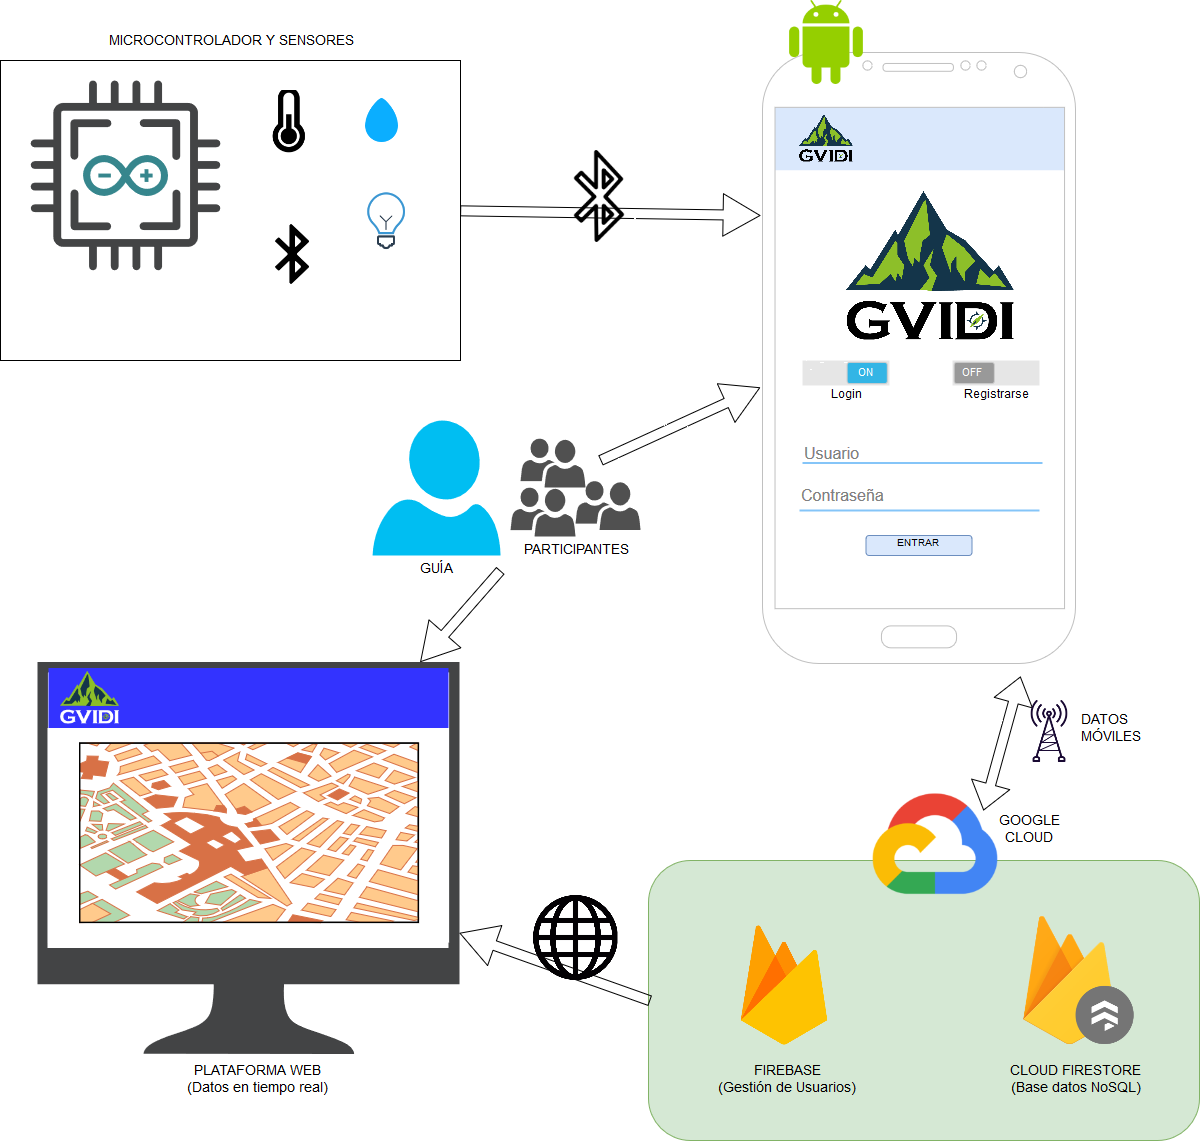
\includegraphics[width=0.75\textwidth]{architecture.png}
\caption{Esquema general de \texttt{GVIDI}.}
\label{fig:esquema}
\end{center}
\end{figure}

De forma global, en \texttt{GVIDI} existen dos roles principales: 

\begin{itemize}
\item \textbf{Guías}. Cada expedición posee un usuario con este rol y será la persona que actué como guía durante la expedición. Recibirá información detallada de todos los participantes durante la expedición, recibiendo alertas ante situaciones de peligro y posibles caídas de los participantes.
\item \textbf{Participantes}. Cada expedición puede poseer varias personas con este rol. Los participantes solo dispondrán de la información relacionada con ellos mismos. Los resultados de su monitorización serán enviados al guía de la expedición.
\end{itemize}

Los guías son los encargados de crear grupos de expedición, a los cuales se pueden unir los participantes. Una expedición está compuesta, por tanto, por un guía y un grupo de participantes. Cada integrante del grupo de expedición portará un microcontrolador en la muñeca, equipado con una serie de sensores que tomarán datos del entorno del integrante (datos de temperatura, humedad, condiciones lumínicas, lluvias, aceleración lineal y angular e información de posición). El microcontrolador se encargará de comunicar toda esta información captada a través de los sensores al dispositivo móvil del integrante, usando un módulo de comunicación \textit{Bluetooth}. En la Tabla \ref{table:componentes} se puede observar el precio de cada uno de los componentes que conforman el dispositivo \textit{hardware}.

\begin{table}[!h]
\centering
\begin{tabular}{@{}lccc@{}}
\rowcolor[HTML]{C0C0C0} 
\multicolumn{1}{c}{\cellcolor[HTML]{C0C0C0}{\color[HTML]{000000} \textbf{Componente}}} & {\color[HTML]{000000} \textbf{Modelo}} & {\color[HTML]{000000} \textbf{Cantidad}} & {\color[HTML]{000000} \textbf{Precio por unidad}} \\ 
\rowcolor[HTML]{EFEFEF} 
Microcontrolador                                                                         & Arduino UNO                            & 3                                        & 24 \euro                                               \\ 
Sensor GPS                                                                               & NEO-6M                                 & 3                                        & 11 \euro                                               \\ 
\rowcolor[HTML]{EFEFEF} 
Sensor pulso cardíaco                                                                    & PulseSensor                            & 3                                        & 6 \euro                                                \\ 
Acelerómetro y giroscopio                                                                & MPU-6050                               & 3                                        & 1.5 \euro                                              \\ 
\rowcolor[HTML]{EFEFEF} 
Sensor de temperatura y humedad                                                          & DHT22                                  & 3                                        & 9.5 \euro                                              \\ 
Detector de lluvia                                                                       & YL-83                                  & 3                                        & 13 \euro                                               \\ 
\rowcolor[HTML]{EFEFEF} 
Fotoresistor Pack 10                                                                     & GL5528                                 & 3                                        & 3 \euro                                                \\ 
Módulo \textit{Bluetooth}                                                                         & HC06                                   & 2                                        & 2.5 \euro                                              \\ 
\end{tabular}
\caption{Componentes que se han usado para construir el prototipo \textit{hardware}.}
\label{table:componentes}
\end{table}

El dispositivo móvil tendrá instalada la aplicación \texttt{GVIDI}, desarrollada durante el presente \ac{TFG}. Esta aplicación posee un sistema de autenticación, usando la plataforma \textit{Firebase Auth}, anteriormente mencionada. El usuario se autenticará en la plataforma y será conducido a la pantalla principal en la que se ve información general sobre el usuario en la aplicación (esta pantalla es igual para todos los roles). Una vez en esta pantalla, las acciones que puede realizar un guía y las que puede realizar un participante de la expedición son distintas y serán expuestas más adelante. De igual forma, los guías serán capaces de crear y finalizar expediciones, mientras que los participantes sólo podrán buscar expediciones en curso y unirse a ellas (o abandonar una expedición a la que se encuentran unidos). Ambos roles pueden ver el estado de la expedición en un mapa, con la localización de todos los participantes de la misma. 

La plataforma \textit{web} también posee el sistema de autenticación usando \textit{Firebase Auth}. En la plataforma \textit{web}, los usuarios pueden ver tanto en tiempo real como a posteriori la expedición realizada (y un histórico de todas las expediciones que el usuario ha realizado, a lo largo del tiempo). La plataforma \textit{web} proporciona información avanzada acerca de la expedición, siendo posible la visualización de estadísticas en un punto determinado de la misma. Gracias a la posibilidad de visualizar la expedición en tiempo real, un familiar o amigo del senderista puede hacer uso de la plataforma \textit{web} para monitorizar el estado de este senderista en la expedición (ver su posición, su velocidad instantánea, la cantidad de distancia que ha recorrido y las alertas que ha generado, ya sea debido a caídas, debido a que ha superado la separación máxima con el guía en algún punto o porque ha solicitado realizar una parada).

\begin{figure}[!h]
\begin{center}
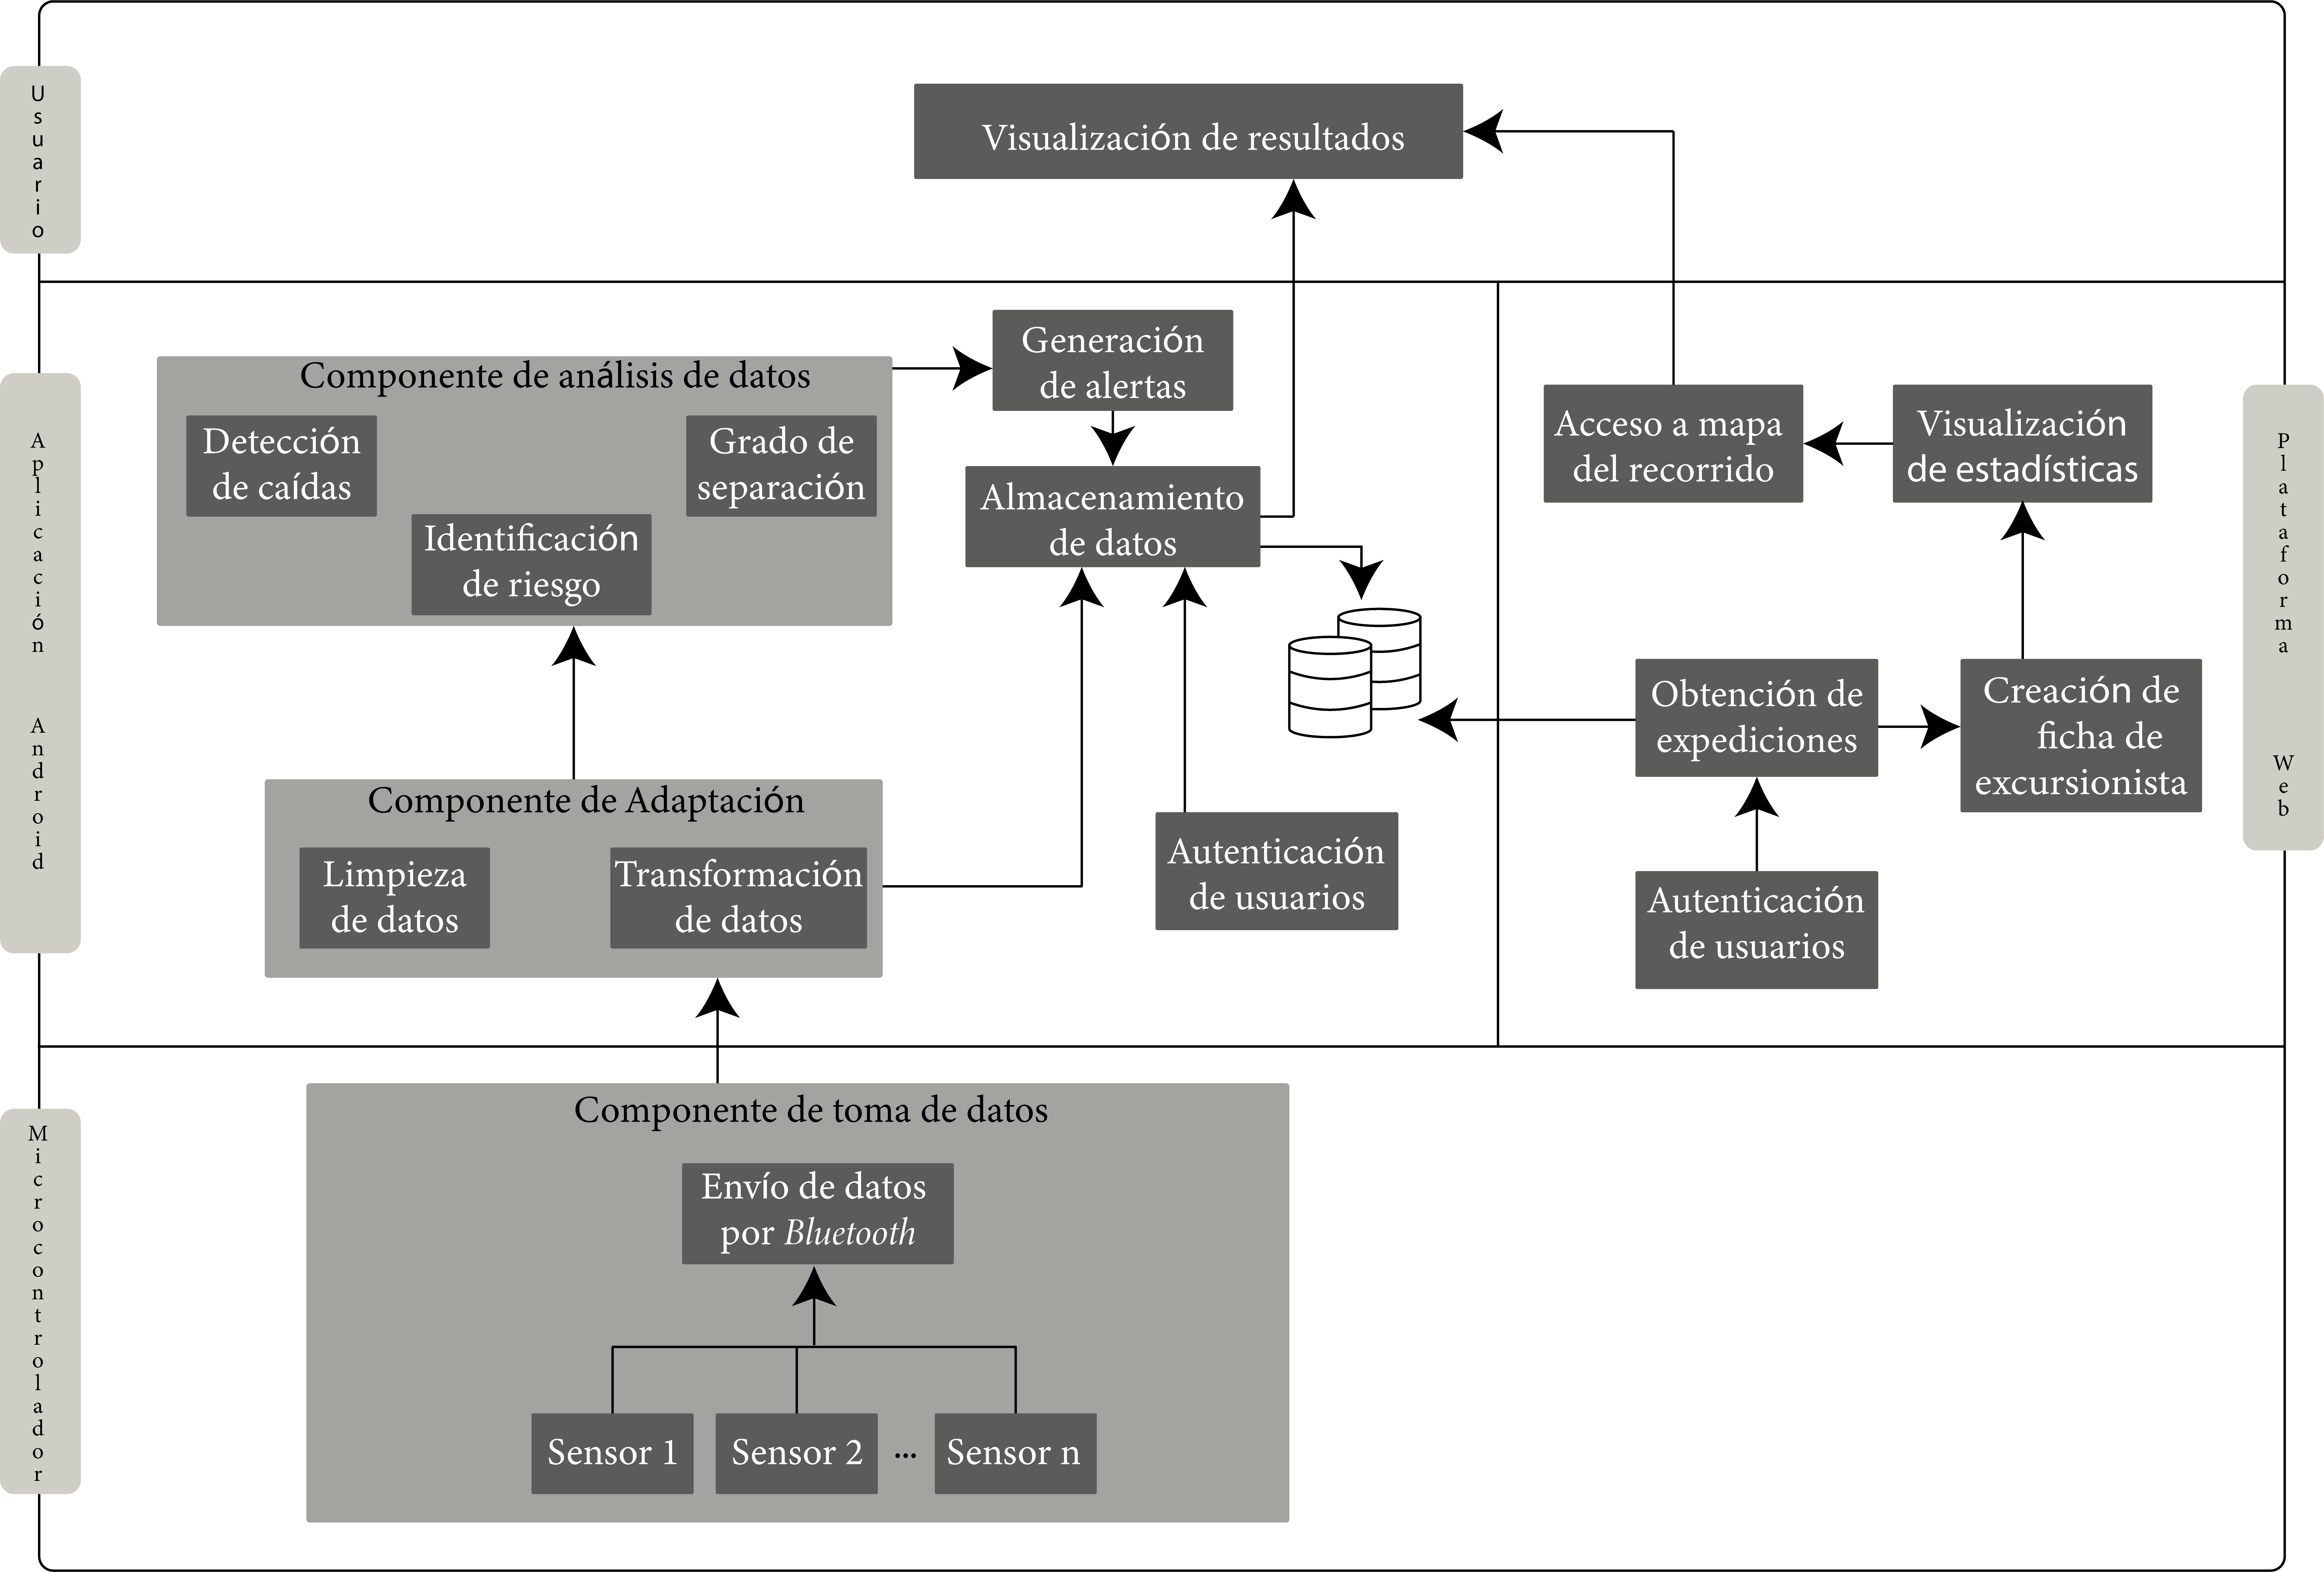
\includegraphics[width=\textwidth]{arquitectura_tfg.png}
\caption{Arquitectura general, en la que se pueden observar los distintos componentes y tareas que conforman el proyecto.}
\label{fig:arquitectura}
\end{center}
\end{figure}

Como se puede observar en la Figura \ref{fig:arquitectura}, se puede dividir la arquitectura general en tres niveles. En el nivel más bajo se situaría el microcontrolador cuya función principal es la comunicación con los distintos sensores que conforman el dispositivo físico, para tomar datos que serán importantes en niveles posteriores. Este nivel es uno de los más importantes porque de él dependen los demás niveles. Se requiere que los datos captados sean lo más fieles a la realidad posibles, que el ruido en estos datos sea el menor posible y que se puedan enviar a una velocidad suficiente para que el análisis en etapas posteriores pueda ser realizado. 

En el siguiente nivel se encuadran la aplicación móvil y la plataforma \textit{web}. El objetivo de este nivel es el manejo de los datos que llegan del nivel previo. En este nivel se realiza un tratamiento y conversión de los datos a un formato para poder almacenarlos directamente o usarlos durante el análisis para producir resultados que serán almacenados más tarde. Los datos se transmiten por un protocolo inalámbrico desde el dispositivo físico a la aplicación móvil (en este proyecto se usa el protocolo \textit{Bluetooth}), por lo que es posible que se produzcan pérdidas de paquetes y lleguen mensajes a la aplicación móvil incompletos o corruptos. Por esto, es necesario realizar una sanitización de los datos previa al tratamiento de estos datos. Además, los datos llegan con unidades distintas a las que requieren los algoritmos de análisis por lo que es necesario realizar un proceso de transformación de datos con el objetivo de que puedan ser usados por dichos algoritmos y puedan ser almacenados en un formato inteligible por los humanos. 

Una vez que los datos han sido correctamente limpiados y transformados, éstos sirven como entrada para los algoritmos de análisis de datos. Estos algoritmos son capaces de inferir si un participante (o guía) de la expedición ha sufrido una caída, determinar el grado de separación del grupo de expedición e identificar el grado de riesgo de sufrir una caída que existe en la expedición en un momento dado, dadas las condiciones ambientales. Las salidas de estos algoritmos sirven para generar alertas si procede, o almacenar las salidas para su posterior uso o visualización. 

En la plataforma \textit{web}, los usuarios de \texttt{GVIDI} podrán acceder al histórico de expediciones en las que el usuario ha participado para ver las estadísticas detalladas de cada una de ellas. También es posible visualizar un mapa con todo el recorrido que el usuario ha realizado y con indicaciones en el mismo acerca del lugar en el que se produjeron las distintas alertas (en el caso de haber alguna). Las alertas también pueden proporcionar información adicional del estado de la expedición en ese momento. Este histórico de expediciones engloba también la expedición que el usuario se encontrase haciendo en el momento (sólo cuando está realizando la expedición), de forma que se puede acceder a toda la información mencionada anteriormente en tiempo real. 

Por último se puede observar el tercer y último nivel de la arquitectura general, que se centra en mostrar información relevante a los usuarios de \texttt{GVIDI}. Esta información se puede mostrar de dos formas distintas, a través de una interfaz de usuario en la aplicación móvil o a través de una página \textit{web}. La primera forma está pensada para que los usuarios de la expedición puedan visualizar durante la expedición información útil para ellos. Por tanto, en la aplicación móvil se tiende a mostrar información en tiempo real y no datos generales de la expedición (el guía tiene una visión más general de la expedición pudiendo ver las alertas generadas en un periodo de tiempo, entre otras opciones). La interfaz de la \textit{web} está pensada para su uso tanto por parte de los usuarios de la ruta como por familiares o amigos de la misma (personas autorizadas por el usuario). En la \textit{web} se pueden visualizar tanto las estadísticas generales de la expedición (en curso o pasada) como la información específica en un punto de la expedición seleccionado.

La arquitectura del presente proyecto no se basa en ningún otro proyecto o aplicación existente, ya que no existen en el mercado alternativas que cumplan con los objetivos de \texttt{GVIDI}. Por tanto, la arquitectura se ha diseñado especialmente para resolver la problemática existente en la monitorización de la seguridad dentro de los grupos de expedición.

En las próximas secciones se describirá con un mayor detalle cada uno de los componentes que forman parte de la arquitectura, así como aspectos del diseño de dichos componentes que se consideren necesarios.

\section{Microcontrolador \textit{Arduino}}

A lo largo de esta sección se presentará con detalle el diseño del microcontrolador \texttt{Arduino} usado en este proyecto. Con este dispositivo se pretende realizar la captación de datos a partir de los sensores que se encuentran equipados en el mismo. En la Tabla \ref{table:magnitudes} se pueden observar los sensores que estarán conectados en el microcontrolador, junto con una breve explicación de para qué se usan los datos que estos sensores captan. 

Para que el dispositivo sea capaz de captar datos de los sensores es necesario implementar la funcionalidad de captación por medio de código fuente usando el lenguaje de programación \texttt{Arduino}, basado en los lenguajes \texttt{C} y \texttt{C++}. A lo largo de esta sección se explicarán los detalles de implementación que se consideren relevantes. 

\begin{table}[!h]
\centering
\begin{tabular}{|l|l|c|}
\hline
\rowcolor[HTML]{656565} 
\multicolumn{1}{|c|}{\cellcolor[HTML]{656565}{\color[HTML]{FFFFFF} Magnitud a medir}} & \multicolumn{1}{c|}{\cellcolor[HTML]{656565}{\color[HTML]{FFFFFF} Propósito de uso del sensor}}                         & {\color[HTML]{FFFFFF} Modelo utilizado} \\ \hline
\rowcolor[HTML]{C0C0C0} 
\begin{tabular}[c]{@{}l@{}}Aceleración y\\ velocidad angular\end{tabular}             & Detección de caídas                                                                                                     & \texttt{MPU6050}       \\ \hline
Temperatura                                                                           & \begin{tabular}[c]{@{}l@{}}Realización del análisis del\\ riesgo de caída en la expedición\end{tabular}                 & \texttt{DHT22}         \\ \hline
\rowcolor[HTML]{C0C0C0} 
Humedad                                                                               & \begin{tabular}[c]{@{}l@{}}Realización del análisis del\\ riesgo de caída en la expedición\end{tabular}                 & \texttt{DHT22}         \\ \hline
                                                                                      & \begin{tabular}[c]{@{}l@{}}Comunicación por \textit{Bluetooth}\\ con el dispositivo móvil\end{tabular} & \texttt{HC-06}         \\ \hline
\rowcolor[HTML]{C0C0C0} 
Lluvia                                                                                & \begin{tabular}[c]{@{}l@{}}Realización del análisis del\\ riesgo de caída en la expedición\end{tabular}                 & \texttt{YL-83}         \\ \hline
Luz                                                                                   & \begin{tabular}[c]{@{}l@{}}Realización del análisis del\\ riesgo de caída en la expedición\end{tabular}                 & \texttt{GL5528}        \\ \hline
\rowcolor[HTML]{C0C0C0} 
Posición                                                                              & \begin{tabular}[c]{@{}l@{}}Localización del participante dentro\\ del grupo de expedición\end{tabular}                  & \texttt{NEO-6M}        \\ \hline
\end{tabular}
\caption{Magnitudes y sensores que se usan en este proyecto.}
\label{table:magnitudes}
\end{table}

\subsection{Diseño del dispositivo \textit{hardware}}

Para el desarrollo de este proyecto se ha usado la placa \texttt{Arduino UNO Rev3}. La placa tiene conectados los siguientes componentes (ver esquema de conexión en la Figura \ref{fig:ard_connections}):

\begin{multicols}{2}
\begin{itemize}
\item Sensor de temperatura y humedad (DHT22)
\item Acelerómetro y giroscopio (MPU6050)
\item Sensor de luminosidad (GL5528)
\item Sensor de lluvia (YL-83)
\item Módulo de \textit{Bluetooth} (HC-06)
\item Sensor de GPS (NEO-6M)
\item Dos resistencias de 10K$\Omega$
\item Dos botones
\item Led de color
\end{itemize}
\end{multicols}

\begin{figure}[!h]
\begin{center}
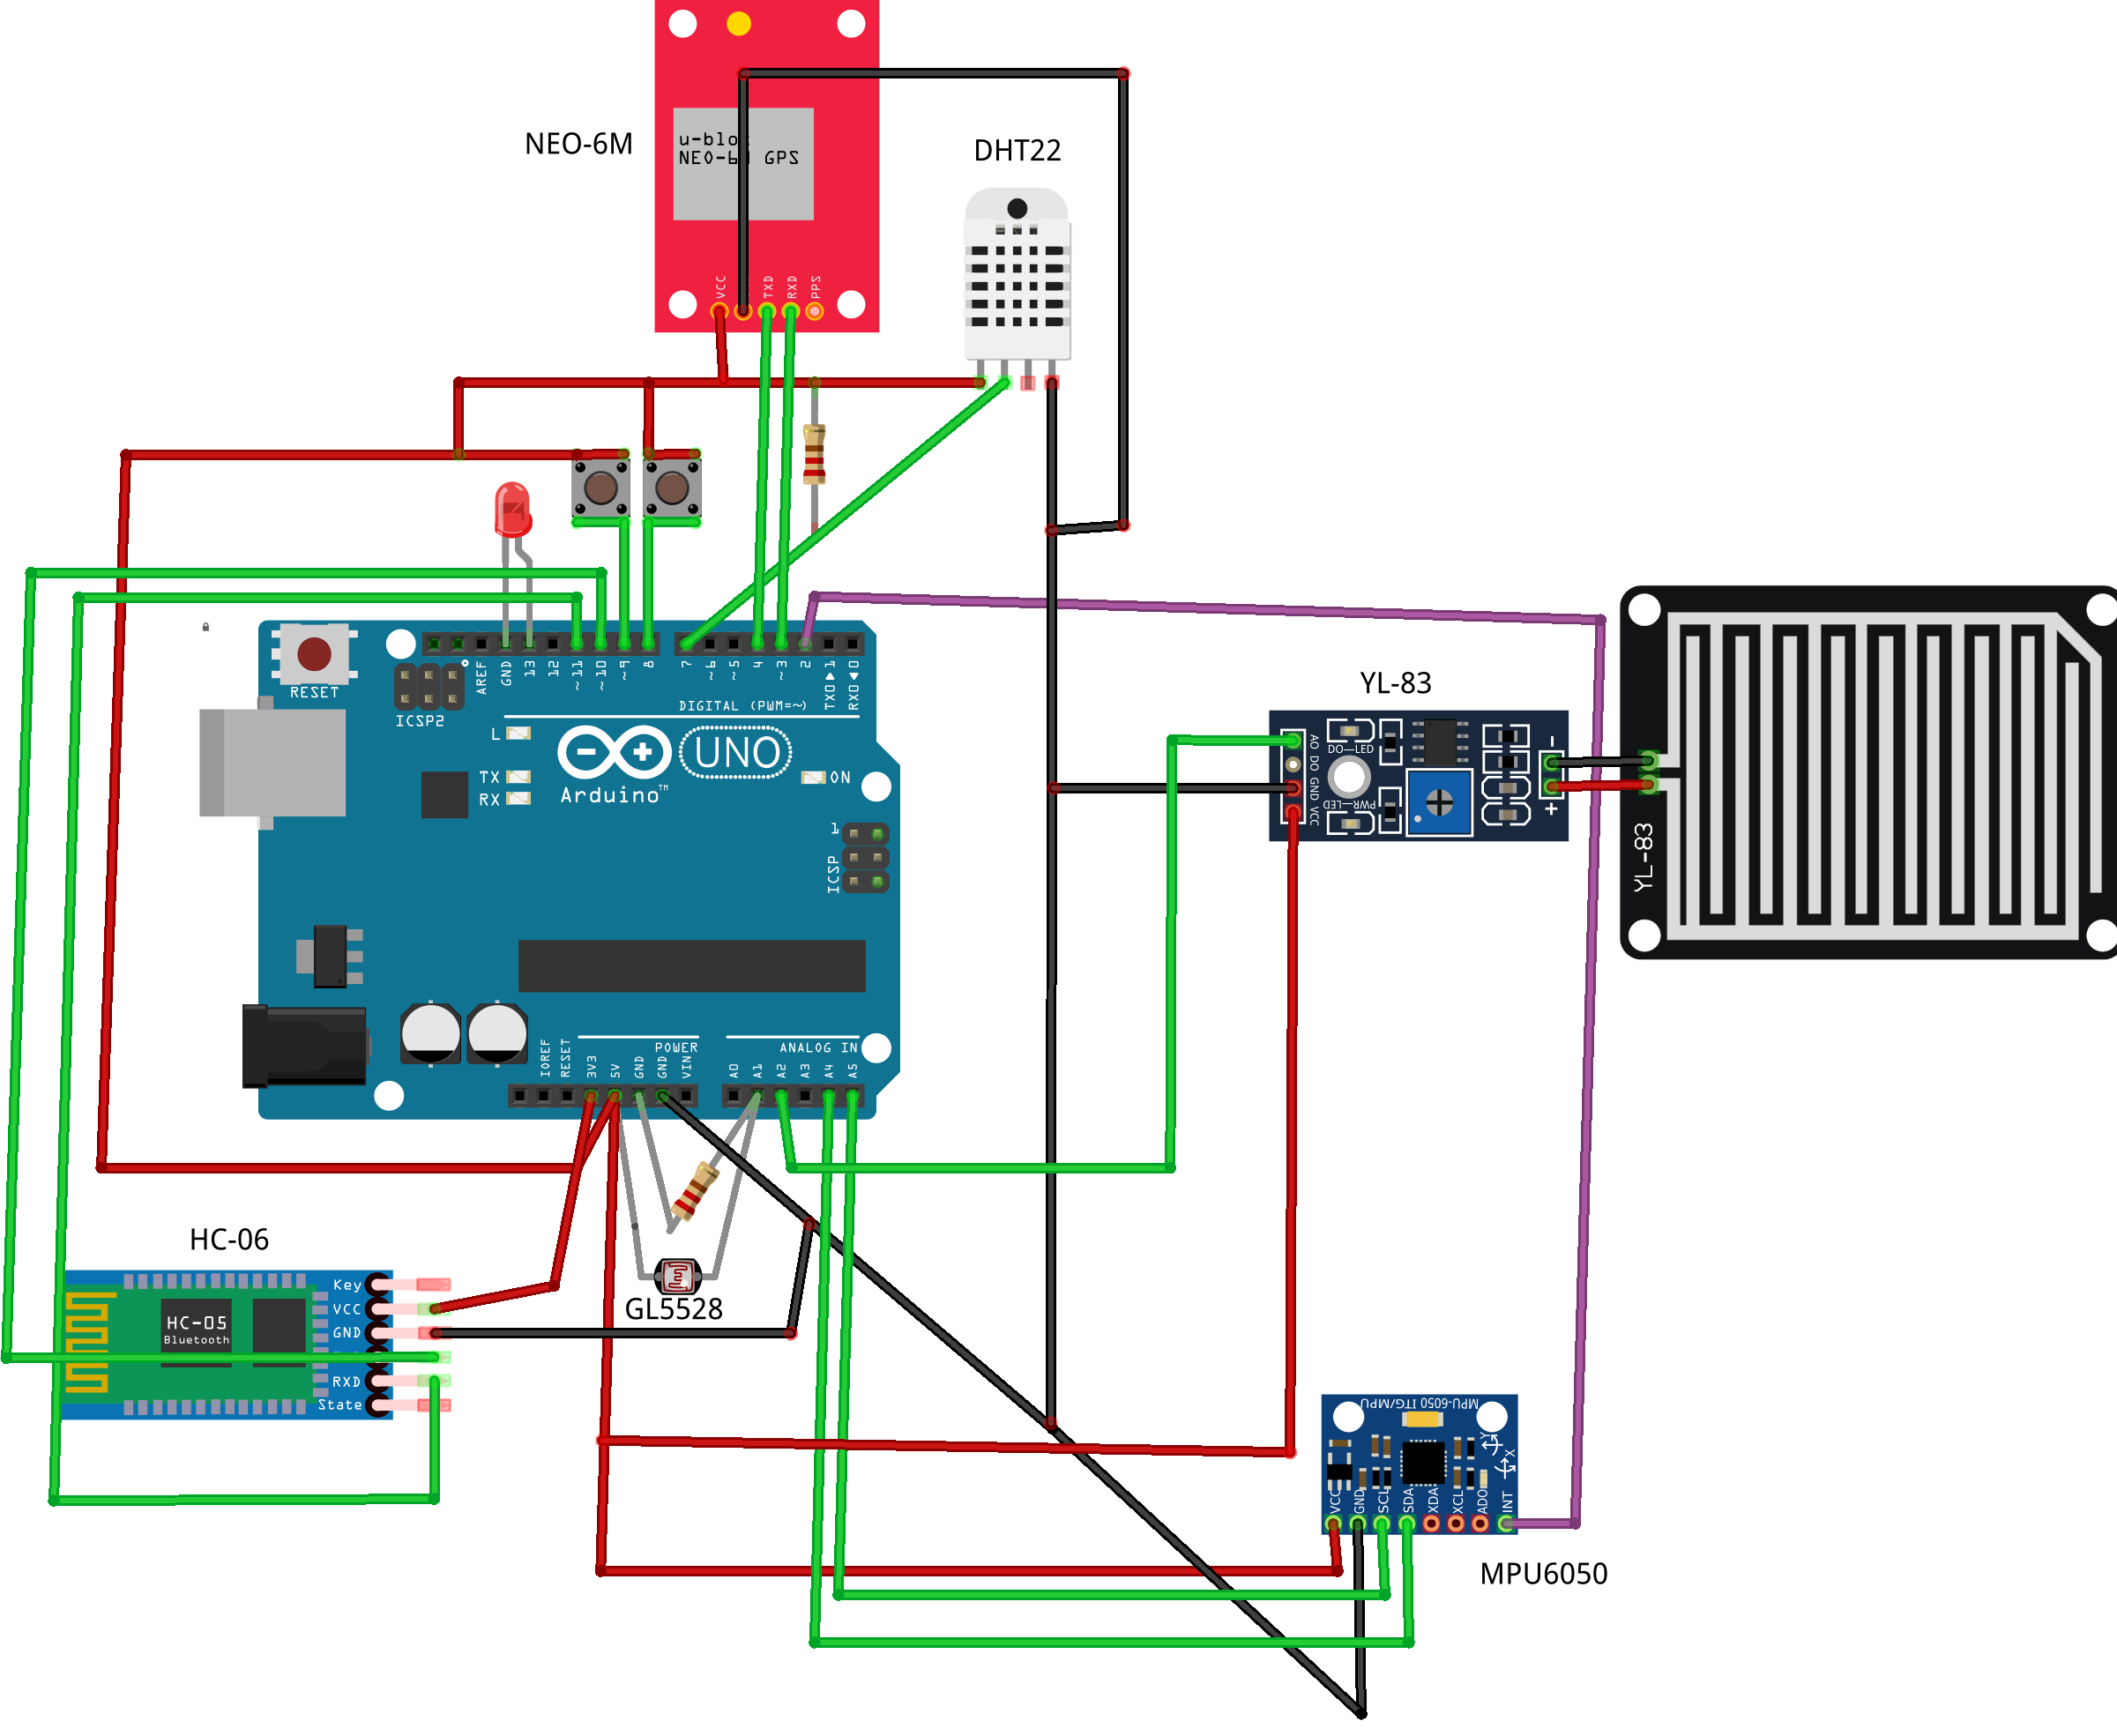
\includegraphics[width=0.75\textwidth]{gvidi_connections.png}
\caption{Conexiones de todos los componenetes en el microcontrolador \texttt{Arduino}.}
\label{fig:ard_connections}
\end{center}
\end{figure}

\subsubsection{Uso de la memoria \ac{EEPROM}}

El microcontrolador \texttt{Arduino UNO} no posee una memoria secundaria como puede tener un ordenador convencional, ni tampoco tiene la posibilidad de introducir una tarjeta \ac{SD} (aunque existen módulos para incorporar esta funcionalidad) como tiene una \texttt{Raspberry Pi}. Por esto, cada vez que el microcontrolador se reinicia, el código que tiene cargado empieza a ejecutarse de nuevo y empezaría otra vez el proceso de calibración del acelerómetro y el giroscopio (explicado en detalle en la sección \ref{ss:implementaciondatos}).

El mayor inconveniente se presenta si, por ejemplo, se reinicia el microcontrolador durante la expedición. Habría que situar el dispositivo en una superficie plana (que puede ser inexistente en ese momento) y esperar un cierto tiempo para realizar la calibración del acelerómetro y giroscopio, por lo que el grupo tendería a dispersarse. Para evitar esta situación se ha hecho uso de la memoria \ac{EEPROM} disponible dentro del procesador. 

Se han almacenado en memoria los datos relativos a la calibración del módulo \texttt{MPU6050} (\textit{offsets} necesarios para calibrar la aceleración en los ejes X, Y, Z y \textit{offsets} necesarios para calibrar la velocidad angular en los ejes X, Y, Z), de tal forma que solo hay que realizar la calibración la primera vez que se usa el dispositivo (también existe la posibilidad de forzar el borrado de la memoria \ac{EEPROM} dejando pulsado un botón en el dispositivo durante más de cinco segundos, como se puede observar en el código del Listado \ref{lst:clearEEPROM}). Se usan un total de 24 \textit{bytes} de memoria \ac{EEPROM} para este cometido (los correspondientes a 6 números en punto flotante), por lo que se trata de una solución óptima a este problema. 

Otras soluciones posibles serían eliminar la posibilidad de almacenar estos \textit{offsets} y dejar que se pudieran dar situaciones potenciales de inusabilidad del dispositivo en plena ruta, o añadir un módulo externo al microcontrolador con una tarjeta \ac{SD}, que implica un menor rendimiento del dispositivo (se emplea mucho tiempo manejando ficheros y el acceso a la tarjeta \ac{SD} es mucho más lento si se compara con el acceso al procesador). Además la cantidad de datos que se almacenan es muy pequeña y no es necesario un gran tamaño de almacenamiento secundario.

\begin{lstlisting}[language=c++,captionpos=t,caption={\textbf{Borrado de la memoria \ac{EEPROM} cuando se deja pulsado un botón durante más de 5 segundos.}},label={lst:clearEEPROM}]
// If the button has been pressed for more than 5 secs, erase EEPROM memory
// and reset the arduino
if(millis() - reset_arduino_pressed_time >= 5000)
{
    eraseEEPROM();
    resetFunction();
}
\end{lstlisting}

Esta memoria tiene un tamaño total de 1024 \textit{bytes} de almacenamiento y tiene unos 100.000 ciclos de lectura/escritura. Esto quiere decir que se puede escribir en la memoria \ac{EEPROM} unas 100.000 veces hasta que esta se vuelva inestable. Esta cantidad de ciclos es más que suficiente para nuestro cometido, ya que simplemente se accederá a la memoria \ac{EEPROM} cada vez que el dispositivo se inicia. 

\subsection{Toma de datos}
\label{ss:implementaciondatos}

Para hacer uso de los distintos sensores se han utilizado librerías programadas en el lenguaje \texttt{C++}. Para algunos sensores se han tomado librerías de código libre, adaptando o añadiendo algunas funciones de las que se hace uso en el proyecto, mientras que para usar otros sensores se ha desarrollado una librería básica. Por ejemplo, la librería usada para tomar datos del sensor de temperatura y humedad \texttt{DHT22}\footnote{\url{https://platformio.org/lib/show/115/DHT22/}} ha sido modificada para añadir una función que devuelve un mensaje de error dependiendo de un código numérico (ver Listado \ref{lst:dht22library}). Esta función fue muy usada durante la primera etapa del proyecto, con un motivo principal de depuración. 

\begin{lstlisting}[language=c++,captionpos=t,caption={\textbf{Ejemplo de funcionalidad añadida a librería de código libre del sensor DHT22.}},label={lst:dht22library}]
void DHT22::getErrorString(DHT22_ERROR_t& errorCode, char* errorString)
{
  switch (errorCode) {
    case DHT_ERROR_CHECKSUM:
      sprintf(errorString, "Error in checksum\n");
      break;
    case DHT_ERROR_TOOQUICK:
      sprintf(errorString, "Wait 2 seconds between each call to readData\n");
      break;
    case DHT_ERROR_NOT_PRESENT:
      sprintf(errorString, "ACK Not Present\n");
      break;
    case DHT_ERROR_ACK_TOO_LONG:
      sprintf(errorString, "ACK too long\n");
      break;
    case DHT_ERROR_DATA_TIMEOUT:
      sprintf(errorString, "Data timeout\n");
      break;
    case DHT_ERROR_SYNC_TIMEOUT:
      sprintf(errorString, "Sync timeout\n");
      break;
  }
\end{lstlisting}

\subsubsection{Temperatura y humedad, \texttt{DHT22}}

\begin{wrapfigure}{r}{0.2\linewidth}
    \centering
    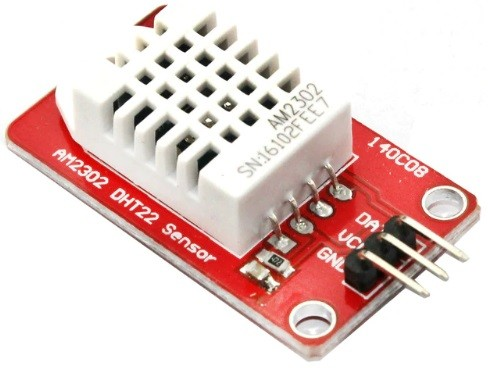
\includegraphics[width=0.2\textwidth]{dht22.jpg}
    \caption{Imagen del sensor \texttt{DHT22} \protect\footnotemark}
    \label{fig:myfig}
\end{wrapfigure}

\footnotetext{Imagen extraída de \url{http://electr3s.com/589/sensor-dht22-digital-de-temperatura-y-humedad.jpg.jpg}}

Haciendo uso de la librería indicada anteriormente, la lectura de valores del sensor \texttt{DHT22} es muy sencilla. Hay que tener en cuenta que el período de sondeo de este sensor es de dos segundos, es decir, realiza una nueva medición de datos de temperatura y humedad cada dos segundos. Si se intentan consultar los datos de temperatura y humedad en un tiempo menor de dos segundos después de la anterior consulta, se devolverá un error.
\begin{lstlisting}[language=c++,captionpos=t,caption={\textbf{Ejemplo de toma de datos del sensor \texttt{DHT22}.}},label={lst:dht22ex}]
#include <DHT22.h>
DHT22 dht22Sensor(DHT22_PIN);
void loop()
{
    DHT22_ERROR_t errorCode;
    // To avoid reading errors
    delay(2000);
    errorCode = dht22Sensor.readData();
    if (errorCode == DHT_ERROR_NONE)
    {
        float temperature = dht22Sensor.getTemperatureC();
        float humidity = dht22Sensor.getHumidity();
    }
}
\end{lstlisting}

\begin{table}[!h]
\centering
\begin{tabular}{l|l|l|l|l|}
\cline{2-5}
                                  & \multicolumn{1}{c|}{\textbf{Valor máximo}}                                                                                                                                & \multicolumn{1}{c|}{\textbf{Valor mínimo}} & \textbf{Precisión}   & \textbf{Periodo de sondeo} \\ \hline
\multicolumn{1}{|l|}{\textbf{Temperatura}} & 80ºC                                                                                                                                                             & -40ºC                             & $\pm 0.5$ºC & 2s                \\ \hline
\multicolumn{1}{|l|}{\textbf{Humedad}}     & 100\%RH\footnote{Humedad relativa. Es la relación entre la presión parcial del vapor de agua y la presión de vapor de equilibrio del agua a una temperatura dada} & 0\%RH                              & $\pm2\%$RH   & 2s                \\ \hline
\end{tabular}
\caption{Características principales del sensor \texttt{DHT22}.}
\label{table:dht22caract}
\end{table}

\subsubsection{Acelerómetro y girsocopio, \texttt{MPU6050}}


El sensor más complejo es el \texttt{MPU6050} (acelerómetro y giroscopio). Para utilizar este sensor, se ha hecho uso de una librería de código libre\footnote{\url{https://github.com/jrowberg/i2cdevlib/tree/master/Arduino/MPU6050}}. Sin embargo, para que las medidas del \texttt{MPU6050} sean fiables y se elimine el ruido en las mismas es necesario calibrar el sensor. Con este módulo es muy posible que exista un desnivel en sus componentes (ver Figura \ref{fig:componentes_mpu6050}). Para eliminar esta desviación en las componentes del módulo y asegurar que no existen desniveles agregados se añaden \textit{offsets}. A cada componente (aceleración en los ejes $X$, $Y$, $Z$ y velocidad angular en los ejes $X$, $Y$, $Z$) se le añadirá un determinado valor, de forma que el sensor en reposo muestre los valores de la Tabla \ref{table:reposo_mpu6050}. 

\begin{wrapfigure}{r}{0.2\linewidth}
    \centering
    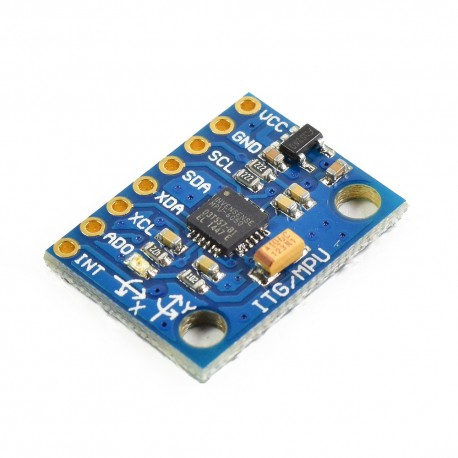
\includegraphics[width=0.2\textwidth]{mpu6050.jpg}
    \caption{Imagen del sensor \texttt{MPU6050} \protect\footnotemark}
    \label{fig:myfig}
\end{wrapfigure}

\footnotetext{Imagen extraída de \\ \url{https://naylampmechatronics.com/763-large_default/modulo-mpu6050-acelerometro-giroscopio-i2c.jpg}}

El módulo en reposo debería mostrar una aceleración neta $| \mathbf{a} | = \sqrt{a_x^2 + a_y^2 + a_z^2} = 1g = 9.8\text{m/s^2}$ y una velocidad angular neta de $0$ $\text{deg/s}$. El valor $16384$ en uno de los ejes indica un valor de $1g$, por lo que para convertir el valor digital que se obtiene del sensor a unidades de $m/s^2$, es necesario aplicar la fórmula: 

\begin{center}
\begin{equation}
$Valor en $m/s^2 = $ valor digital $\cdot (9.81 / 16384)
\end{equation}
\end{center}

\begin{table}[!h]
\centering
\begin{tabular}{cl|l|l|l|}
\cline{3-5}
\multicolumn{1}{l}{}                                     &       & \multicolumn{3}{c|}{\textbf{Valores digitales de salida del sensor}}                                \\ \cline{3-5} 
\multicolumn{1}{l}{}                                     &       & \multicolumn{1}{c|}{\textbf{En reposo}} & \multicolumn{1}{c|}{\textbf{Máximo}} & \multicolumn{1}{c|}{\textbf{Mínimo}} \\ \hline
\multicolumn{1}{|c|}{\multirow{}{}{\textbf{Aceleración}}}       & \textbf{Eje X} & 16384 $\pm 8 = 1g$             & 32767 $= 2g$                & -32768 $= -2g$              \\ \cline{2-5} 
\multicolumn{1}{|c|}{}                                   & \textbf{Eje Y }& 0 $\pm 8 = 0g$                 & 32767 $= 2g$                & -32768 $= -2g$              \\ \cline{2-5} 
\multicolumn{1}{|c|}{}                                   & \textbf{Eje Z }& 0 $\pm 8 = 0g$                 & 32767 $= 2g$                & -32768 $= -2g$              \\ \hline
\multicolumn{1}{|c|}{\multirow{}{}{\textbf{Velocidad angular}}} & \textbf{Eje X} & 0 $\pm 1 = 0deg/s$             & 32767 $= 250deg/s$          & -32768 $= -250deg/s$        \\ \cline{2-5} 
\multicolumn{1}{|c|}{}                                   & \textbf{Eje Y} & 0 $\pm 1 = 0deg/s$             & 32767 $= 250deg/s$          & -32768 $= -250deg/s$        \\ \cline{2-5} 
\multicolumn{1}{|c|}{}                                   & \textbf{Eje Z} & 0 $\pm 1 = 0deg/s$             & 32767 $= 250deg/s$          & -32768 $= -250deg/s$        \\ \hline
\end{tabular}
\caption{Valores digitales que mide el sensor \texttt{MPU6050} para una sensibilidad de $\pm 2g$ en la aceleración y de $\pm 250$ $deg/s$ en la velocidad angular.}
\label{table:reposo_mpu6050}
\end{table}

\paragraph{Calibración del módulo \texttt{MPU6050}.}

La calibración es un proceso por el cual se toman un gran número de medidas del módulo, se descartan las primeras medidas (un total de 100 en el caso de este proyecto) para evitar ruido y se calcula el valor medio entre las medidas que se han tomado. Con este valor medio calculado se proceden a calcular los valores de \textit{offset} (véase Listado \ref{lst:offset_calc}), que serán aplicados al sensor. Este proceso se repetirá hasta que las medias de las medidas en todas las componentes del módulo estén dentro de un determinado umbral, próximo a los valores mostrados en la Tabla \ref{table:reposo_mpu6050}. Se establece un umbral debido a que es posible que los valores de las medias de las medidas nunca llegen a converger hasta llegar a los valores exactos mostrados en la tabla. Los umbrales que se ha decidido tomar por defecto son $\pm 8$ para la aceleración y $\pm 1$ para la velocidad angular.

\begin{lstlisting}[language=c++,captionpos=t,caption={\textbf{Cálculo de los \textit{offsets} (en este ejemplo se han sustituido las constantes por números para un mejor entendimiento).}},label={lst:offset_calc}]
ax_offset = (16384 - mean_ax) / 8;
ay_offset = - mean_ay / 8;
az_offset = - mean_az / 8;

gx_offset = -mean_gx / 4;
gy_offset = -mean_gy / 4;
gz_offset = -mean_gz / 4;
while (1){
  int ready = 0;
  mpu6050_sensor.setXAccelOffset(ax_offset);
  mpu6050_sensor.setYAccelOffset(ay_offset);
  mpu6050_sensor.setZAccelOffset(az_offset);

  mpu6050_sensor.setXGyroOffset(gx_offset);
  mpu6050_sensor.setYGyroOffset(gy_offset);
  mpu6050_sensor.setZGyroOffset(gz_offset);

  TakeAMeasurement();
    
  // Check if all the offsets are ok. If only one of the offset is not ok,
  // correct the offset and take measures again
  if ((abs(16384 - mean_ax)) <= 8) ready++;
  else ax_offset = ax_offset + (16384 - mean_ax) / 8;

  if (abs(mean_ay) <= 8) ready++;
  else ay_offset = ay_offset - mean_ay / 8;

  if (abs(mean_az) <= 8) ready++;
  else az_offset = az_offset - mean_az / 8;
	
  if (abs(mean_gx) <= 1) ready++;
  else gx_offset = gx_offset - mean_gx / (1 + 1);

  if (abs(mean_gy) <= 1) ready++;
  else gy_offset = gy_offset - mean_gy / (1 + 1);

  if (abs(mean_gz) <= 1) ready++;
  else gz_offset = gz_offset - mean_gz / (1 + 1);
  
  if (ready == 6) break;
}
\end{lstlisting}

La calibración es un proceso que necesita realizarse con el microcontrolador totalmente en reposo, sobre una superficie lo más plana posible. Este proceso se realiza nada mas conectar el microcontrolador y puede llevar un tiempo arbitrario que puede llegar a ser bastante elevado (durante el desarrollo del proyecto se han podido observar valores que oscilaban entre los 20 segundos a los 5 minutos). El motivo por el cual el proceso de calibración oscila entre unos valores tan dispares es el proceso de cálculo de \textit{offsets}, que se puede observar en el código del Listado \ref{lst:offset_calc}. Como se puede observar, este cálculo depende del \textit{offset} calculado anteriormente y de la media de un cierto número de medidas que se han realizado con el sensor. Si el sensor no se encuentra en completo reposo (o sobre una superficie lo suficientemente plana) la media de los valores de aceleración no será todo lo próxima necesaria al valor de 1g (o $9.8m/s^2$). Por ejemplo, mientras la media de los valores de la acelaración en el eje Z no esté en el intervalo [-8, 8], el \textit{offset} para la aceleración en este eje no será correcto y el proceso de calibración no finalizará. El sensor también puede realizar alguna medida errónea en un momento dado (lo que consideraríamos ruido), que afecta negativamente al proceso de calibración. Las medidas erróneas por parte del sensor no tienen una solución sencilla por lo que se asume que el sensor no realizará mediciones incorrectas. En el caso de realizarlas, el algoritmo anterior se encarga de gestionarlas ya que no finalizará hasta que el módulo esté completamente calibrado.

\begin{figure}[!h]
\begin{center}
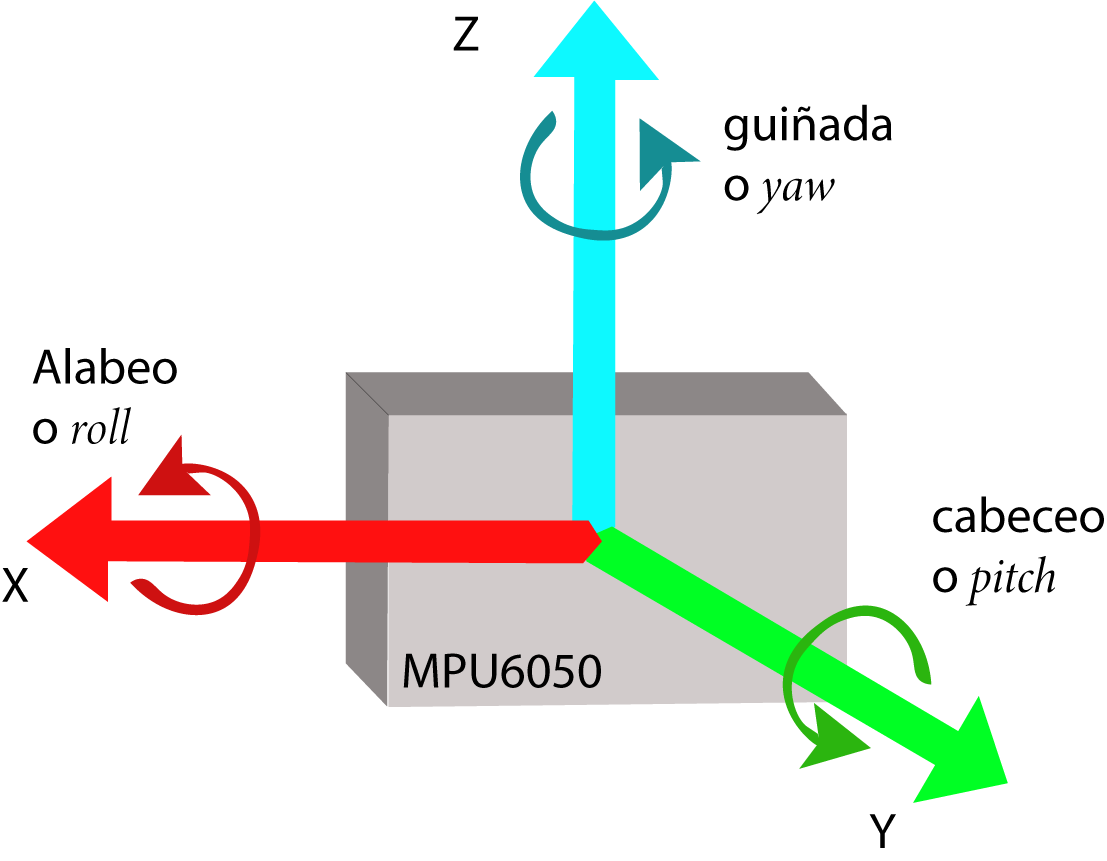
\includegraphics[width=0.5\textwidth]{componentes_mpu6050.png}
\caption{Componentes del acelerómetro y giroscopio \texttt{MPU6050}.}
\label{fig:componentes_mpu6050}
\end{center}
\end{figure}

Una vez realizada la calibración del módulo \texttt{MPU6050}, ya puede ser usado de forma habitual. En este proyecto simplemente se solicitan los valores actuales de aceleración y velocidad angular, que serán utilizados en el análisis inteligente de los datos.

\subsubsection{Sensor de lluvia, \texttt{YL-83}}


El uso del sensor de lluvia es muy simple. Este sensor está conectado a una entrada analógica y devuelve un valor de voltaje que va desde 0 para una placa completamente mojada hasta 1023 para una placa completamente seca. Este sensor no posee la precisión necesaria para medir la cantidad de agua acumulada, por lo que tan sólo es útil para medir la presencia o ausencia de agua. En nuestro caso la información de si está lloviendo o no es suficiente para ser usada posteriormente en el análisis del riesgo de caída en la expedición.


\begin{figure}[!h]
    \centering
    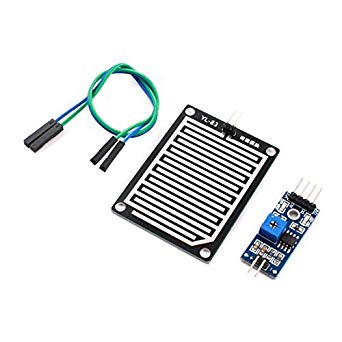
\includegraphics[width=0.2\textwidth]{yl83.jpg}
    \caption{Imagen del sensor de lluvia \texttt{YL-83} \protect\footnotemark}
    \label{fig:myfig}
\end{figure}

\footnotetext{Imagen extraída de \url{https://images-na.ssl-images-amazon.com/images/I/51SeX9Bk7kL._SX342_.jpg}}

Para hacer uso de este sensor se ha creado una librería realmente simple, que lee el valor analógico proporcionado por el sensor y devuelve un valor que indica la cantidad aproximada de lluvia que hay. La Tabla \ref{table:yl83lib} muestra la salida de la librería para los distintos valores obtenidos del sensor.

\begin{table}[!h]
\centering
\begin{tabular}{l|l|l|l|l|}
\cline{2-5}
                                           & \textbf{No hay lluvia}                      & \textbf{Lluvia suave}                      & \textbf{Lluvia moderada}                   & \textbf{Lluvia fuerte}                   \\ \hline
\multicolumn{1}{|l|}{\textbf{Intervalo de valores}} & \multicolumn{1}{c|}{$[500, 1023]$} & \multicolumn{1}{c|}{$(300, 500)$} & \multicolumn{1}{c|}{$[300, 100)$} & \multicolumn{1}{c|}{$[0, 100]$} \\ \hline
\end{tabular}
\caption{Intervalos de voltaje que el sensor \texttt{YL-83} proporciona y su relación con la cantidad aproximada de lluvia.}
\label{table:yl83lib}
\end{table}

\subsubsection{Sensor \ac{GPS}, \texttt{NEO-6M}}

\begin{wrapfigure}{r}{0.2\linewidth}
    \centering
    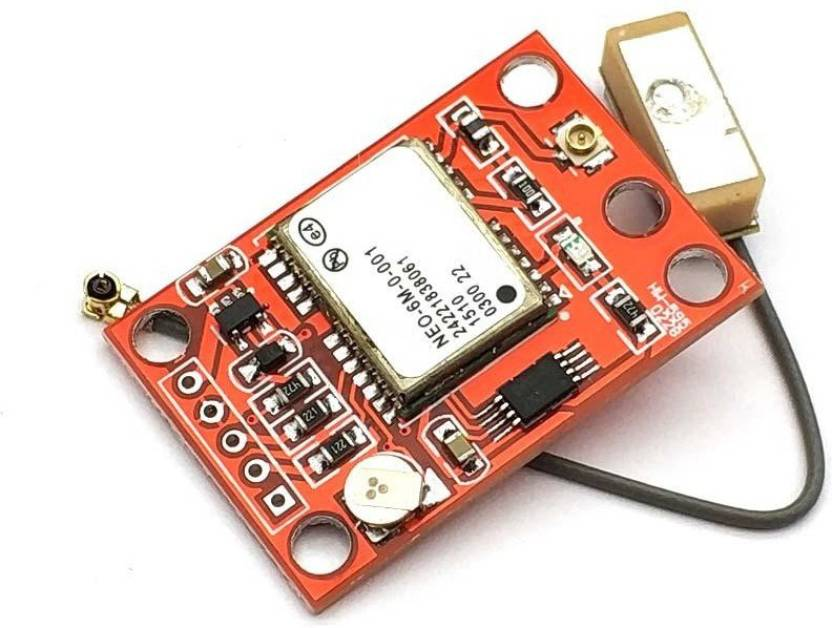
\includegraphics[width=0.2\textwidth]{neo6m.jpeg}
    \caption{Imagen del sensor \texttt{NEO-6M} \protect\footnotemark}
    \label{fig:myfig}
\end{wrapfigure}

\footnotetext{Imagen extraída de \url{https://rukminim1.flixcart.com/image/832/832/joonafk0/electronic-hobby-kit/d/z/6/neo6m-gps-module-flight-controller-arduino-original-imafb2yyz9xudsfj.jpeg?q=70}}

Para hacer uso de este sensor se ha usado la librería \texttt{TinyGPS}\footnote{\url{http://arduiniana.org/libraries/tinygps/}}. La librería no es necesaria para tomar datos del sensor pero es una gran ayuda para identificar los datos que se obtienen del sensor y mostrarlos de forma entendible. Este sensor posee una antena cerámica para captar la información de los satélites y se conecta al microcontrolador a través de una conexión serial (usando dos pines, uno para transmisión y otro para recepción). Los pines usados para la conexión serial del módulo de \ac{GPS} son los pines 3 y 4, como se puede ver en el esquema de conexión de la Figura \ref{fig:ard_connections}.

Los datos que se obtienen de la lectura serial del sensor están en formato \ac{NMEA} (véase Listado \ref{lst:nmeavals}). Existen varios mensajes \ac{GPS} \ac{NMEA}, como \$GPGGA que proporciona datos de localización y precisión, \$GPGSV que proporciona información de satélites o \$GPGLL que proporciona datos de latitud y longitud geográfica, entre otros. En este punto es donde la librería \texttt{TinyGPS} entra en juego, facilitando la tarea de entendimiento de los mensajes \ac{NMEA}. En el Listado \ref{lst:neo6mread} se puede observar la sencillez para obtener la posición actual a partir de las sentencias \ac{NMEA} usando esta librería.

\begin{lstlisting}[language=c++,captionpos=t,caption={\textbf{Lectura de datos del módulo GPS usando una comunicación serial.}},label={lst:neo6mread}]
// This function reads data from the GPS sensor
void readGPSData(float* latitude, float* longitude)
{
  while (ss_gps.available())
  {
    char c = ss_gps.read();   // Serial read to get the gps data
    if (tinyGPSInstance.encode(c))   // Did a new valid sentence come in?
    {
      tinyGPSInstance.f_get_position(latitude, longitude);
    }
  }
}
\end{lstlisting}

\begin{lstlisting}[language=c++,captionpos=t,caption={\textbf{Ejemplo de valores en formato \ac{NMEA}.}},label={lst:nmeavals}]
$GPGGA,110617.00,41XX.XXXXX,N,00831.54761,W,1,05,2.68,129.0,M,50.1,M,,*42
$GPGSA,A,3,06,09,30,07,23,,,,,,,,4.43,2.68,3.53*02
$GPGSV,3,1,11,02,48,298,24,03,05,101,24,05,17,292,20,06,71,227,30*7C
$GPGSV,3,2,11,07,47,138,33,09,64,044,28,17,01,199,,19,13,214,*7C
$GPGSV,3,3,11,23,29,054,29,29,01,335,,30,29,167,33*4E
$GPGLL,41XX.XXXXX,N,00831.54761,W,110617.00,A,A*70
$GPRMC,110618.00,A,41XX.XXXXX,N,00831.54753,W,0.078,,030118,,,A*6A 
$GPVTG,,T,,M,0.043,N,0.080,K,A*2C
\end{lstlisting}

\paragraph{Problema en el uso del sensor de \ac{GPS}.}

Ha habido un problema durante la integración del módulo de \ac{GPS} relacionado con la captación de datos, que no ha hecho posible su uso. Al intentar tomar los datos de latitud y longitud del módulo, se obtenía un resultado igual que el que se obtendría si el módulo no pudiese comunicarse con ningún satélite. En un principio se pensó que era debido a una falta de cobertura, ya que es necesario esperar unos minutos con el módulo al aire libre para que pueda comenzar a tomar datos con normalidad. Después de dejar el prototipo al aire libre en distintas ocasiones y localizaciones (entre ellas Madrid, donde la captación de señal no debería ser un problema para el módulo) durante un período prolongado de tiempo, ha sido imposible captar señal \ac{GPS}. Al inicio del proyecto se compraron tres módulos \ac{GPS}, uno para cada uno de los prototipos que se van a crear durante el presente proyecto. Al recibirlos, uno de los módulos venía con signos evidentes de corrosión y con la antena desoldada de la placa por lo que se piensa que el motivo por el cual los dos módulos restantes no funcionan es debido a que están defectuosos.

Para resolver esta problemática se ha hecho uso del \ac{GPS} del dispositivo móvil para tomar los datos relativos a la posición del guía y de los participantes en la expedición (se explicará en más detalle en la sección relacionada con la arquitectura de la aplicación móvil). Sin embargo, el código fuente del microcontrolador contempla la toma de datos a través de un módulo \ac{GPS} \texttt{NEO-6M} conectado al mismo (y el envío de los mismos al dispositivo móvil usando \textit{Bluetooth}) y la \ac{PCB} ha sido diseñada con las conexiones necesarias para integrar dicho módulo. Por esto, debería bastar con conectar un módulo \ac{GPS} válido a la \ac{PCB} y esperar a que el mismo capte señal para que la información de posición sea la dictada por el microcontrolador en vez de la dictada por el dispositivo móvil. 

\subsection{Creación de la \ac{PCB}}

Durante la etapa inicial del proyecto, en la que se desarrolló el código fuente que usa el dispositivo para comunicarse con los distintos sensores que posee, se hizo uso de una placa \textit{protoboard}, en la que se conectaban todos los sensores al microcontrolador por medio de cables de prototipado. De esta forma, era muy sencillo realizar cambios debidos a fallos en la conexión (si se conecta un sensor a un \textit{pin} erróneo del microcontrolador) y añadir nuevos componentes (como es el caso de los botones y los leds) si eran requeridos en versiones posteriores del dispositivo.

Una vez se obtuvo una versión definitiva del dispositivo, se pensó en crear una \ac{PCB} para mejorar la presentación del mismo. Usando una \ac{PCB}, se eliminan los cables de prototipado y la placa \textit{protoboard}, quedando un diseño mucho más profesional. Además, se elimina la posibilidad de que en plena ruta un usuario desconecte un cable del microcontrolador o de la placa \textit{protoboard} y no sepa dónde conectarlo después. Esta situación podría dar lugar a que un sensor deje de funcionar o, en el peor de los casos, que un sensor resulte dañado si se conecta de forma errónea. 

Para el diseño de la \ac{PCB} se ha usado el \textit{software} de código libre \texttt{KiCad}\footnote{\url{http://kicad-pcb.org/}}. Una \ac{PCB} básica posee un total de dos capas, la superior y la inferior. Ambas capas se pueden usar para el rutado entre los componentes de la misma y se comunican a través de vías, que son pequeños agujeros en la placa que comunican la capa superior con la capa inferior de la misma. En la Figura \ref{fig:pcb_design} se puede observar el diseño de ambas capas de la placa. En este diseño se encuentran los orificios necesarios para conectar la \ac{PCB} con el microcontrolador, los orificios necesarios para conectar todos los sensores en la placa y además, las rutas entre el microcontrolador y los sensores. También se ha dotado al diseño de etiquetas para identificar los sensores, además del logo del proyecto para garantizar la propiedad del mismo. 

\begin{figure}
 \centering
  \subfloat[Capa superior.]{
   \label{fig:inf_design}
    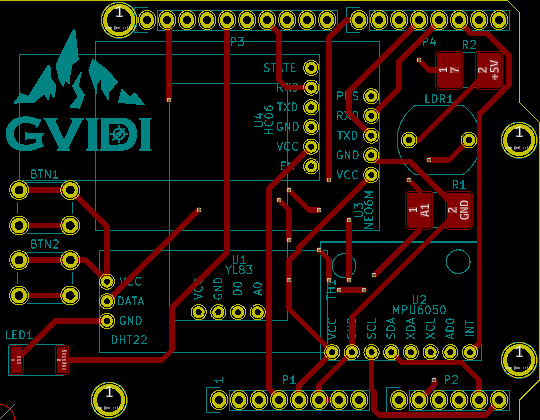
\includegraphics[width=0.45\textwidth]{pcb_suplay_design.png}}
  \subfloat[Capa inferior.]{
   \label{fig:sup_design}
    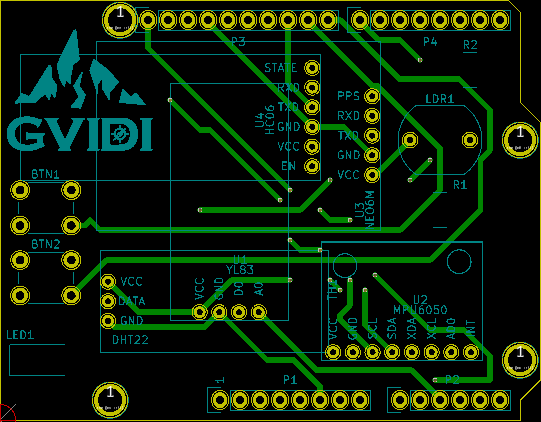
\includegraphics[width=0.45\textwidth]{pcb_inflay_design.png}}
 \caption{Diseño de la \ac{PCB}.}
 \label{fig:pcb_design}
\end{figure}

\begin{figure}
 \centering
  \subfloat[Capa superior.]{
   \label{fig:inf_render}
    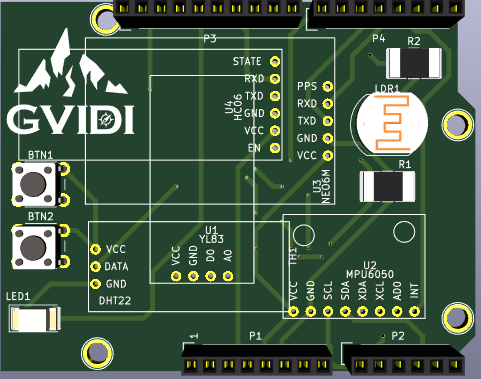
\includegraphics[width=0.45\textwidth]{pcb_suplay_render.png}}
  \subfloat[Capa inferior.]{
   \label{fig:sup_render}
    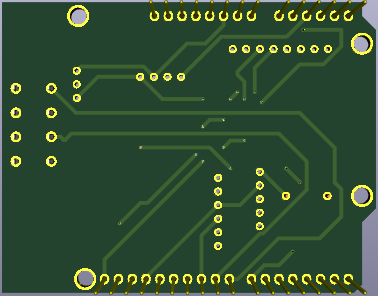
\includegraphics[width=0.45\textwidth]{pcb_inflay_render.png}}
 \caption{Vista en 3D de la \ac{PCB}.}
 \label{fig:pcb_render}
\end{figure}

Una vez se ha completado el diseño de la \ac{PCB}, es necesario crearla físicamente. La impresión de la \ac{PCB} ha sido realizada por una empresa que se dedica a ello. El resultado final es el que se ve en la Figura \ref{fig:pcb_final}. El ultimo paso es soldar en la placa todos los sensores y actuadores que se usan en este proyecto, además de los pines necesarios para conectar la placa en el microcontrolador. En la Figura \ref{fig:prototype} se puede observar la versión final del prototipo desarrollado durante este proyecto.

\begin{figure}
 \centering
  \subfloat[Capa superior.]{
   \label{fig:sup_final}
    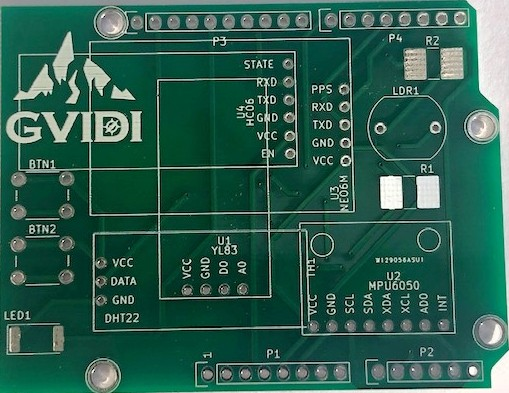
\includegraphics[width=0.45\textwidth]{pcb_sup_final.jpg}}
  \subfloat[Capa inferior.]{
  \label{fig:inf_final}
    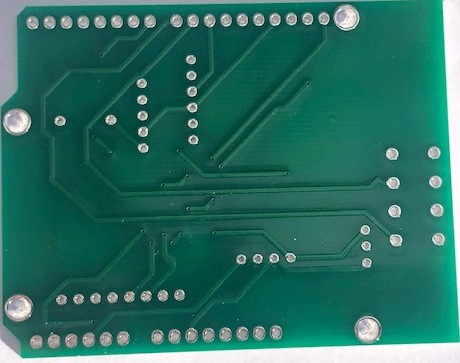
\includegraphics[width=0.45\textwidth]{pcb_inf_final.jpg}}
 \caption{Impresión final de la \ac{PCB}.}
 \label{fig:pcb_final}
\end{figure}

\begin{figure}[!h]
\begin{center}
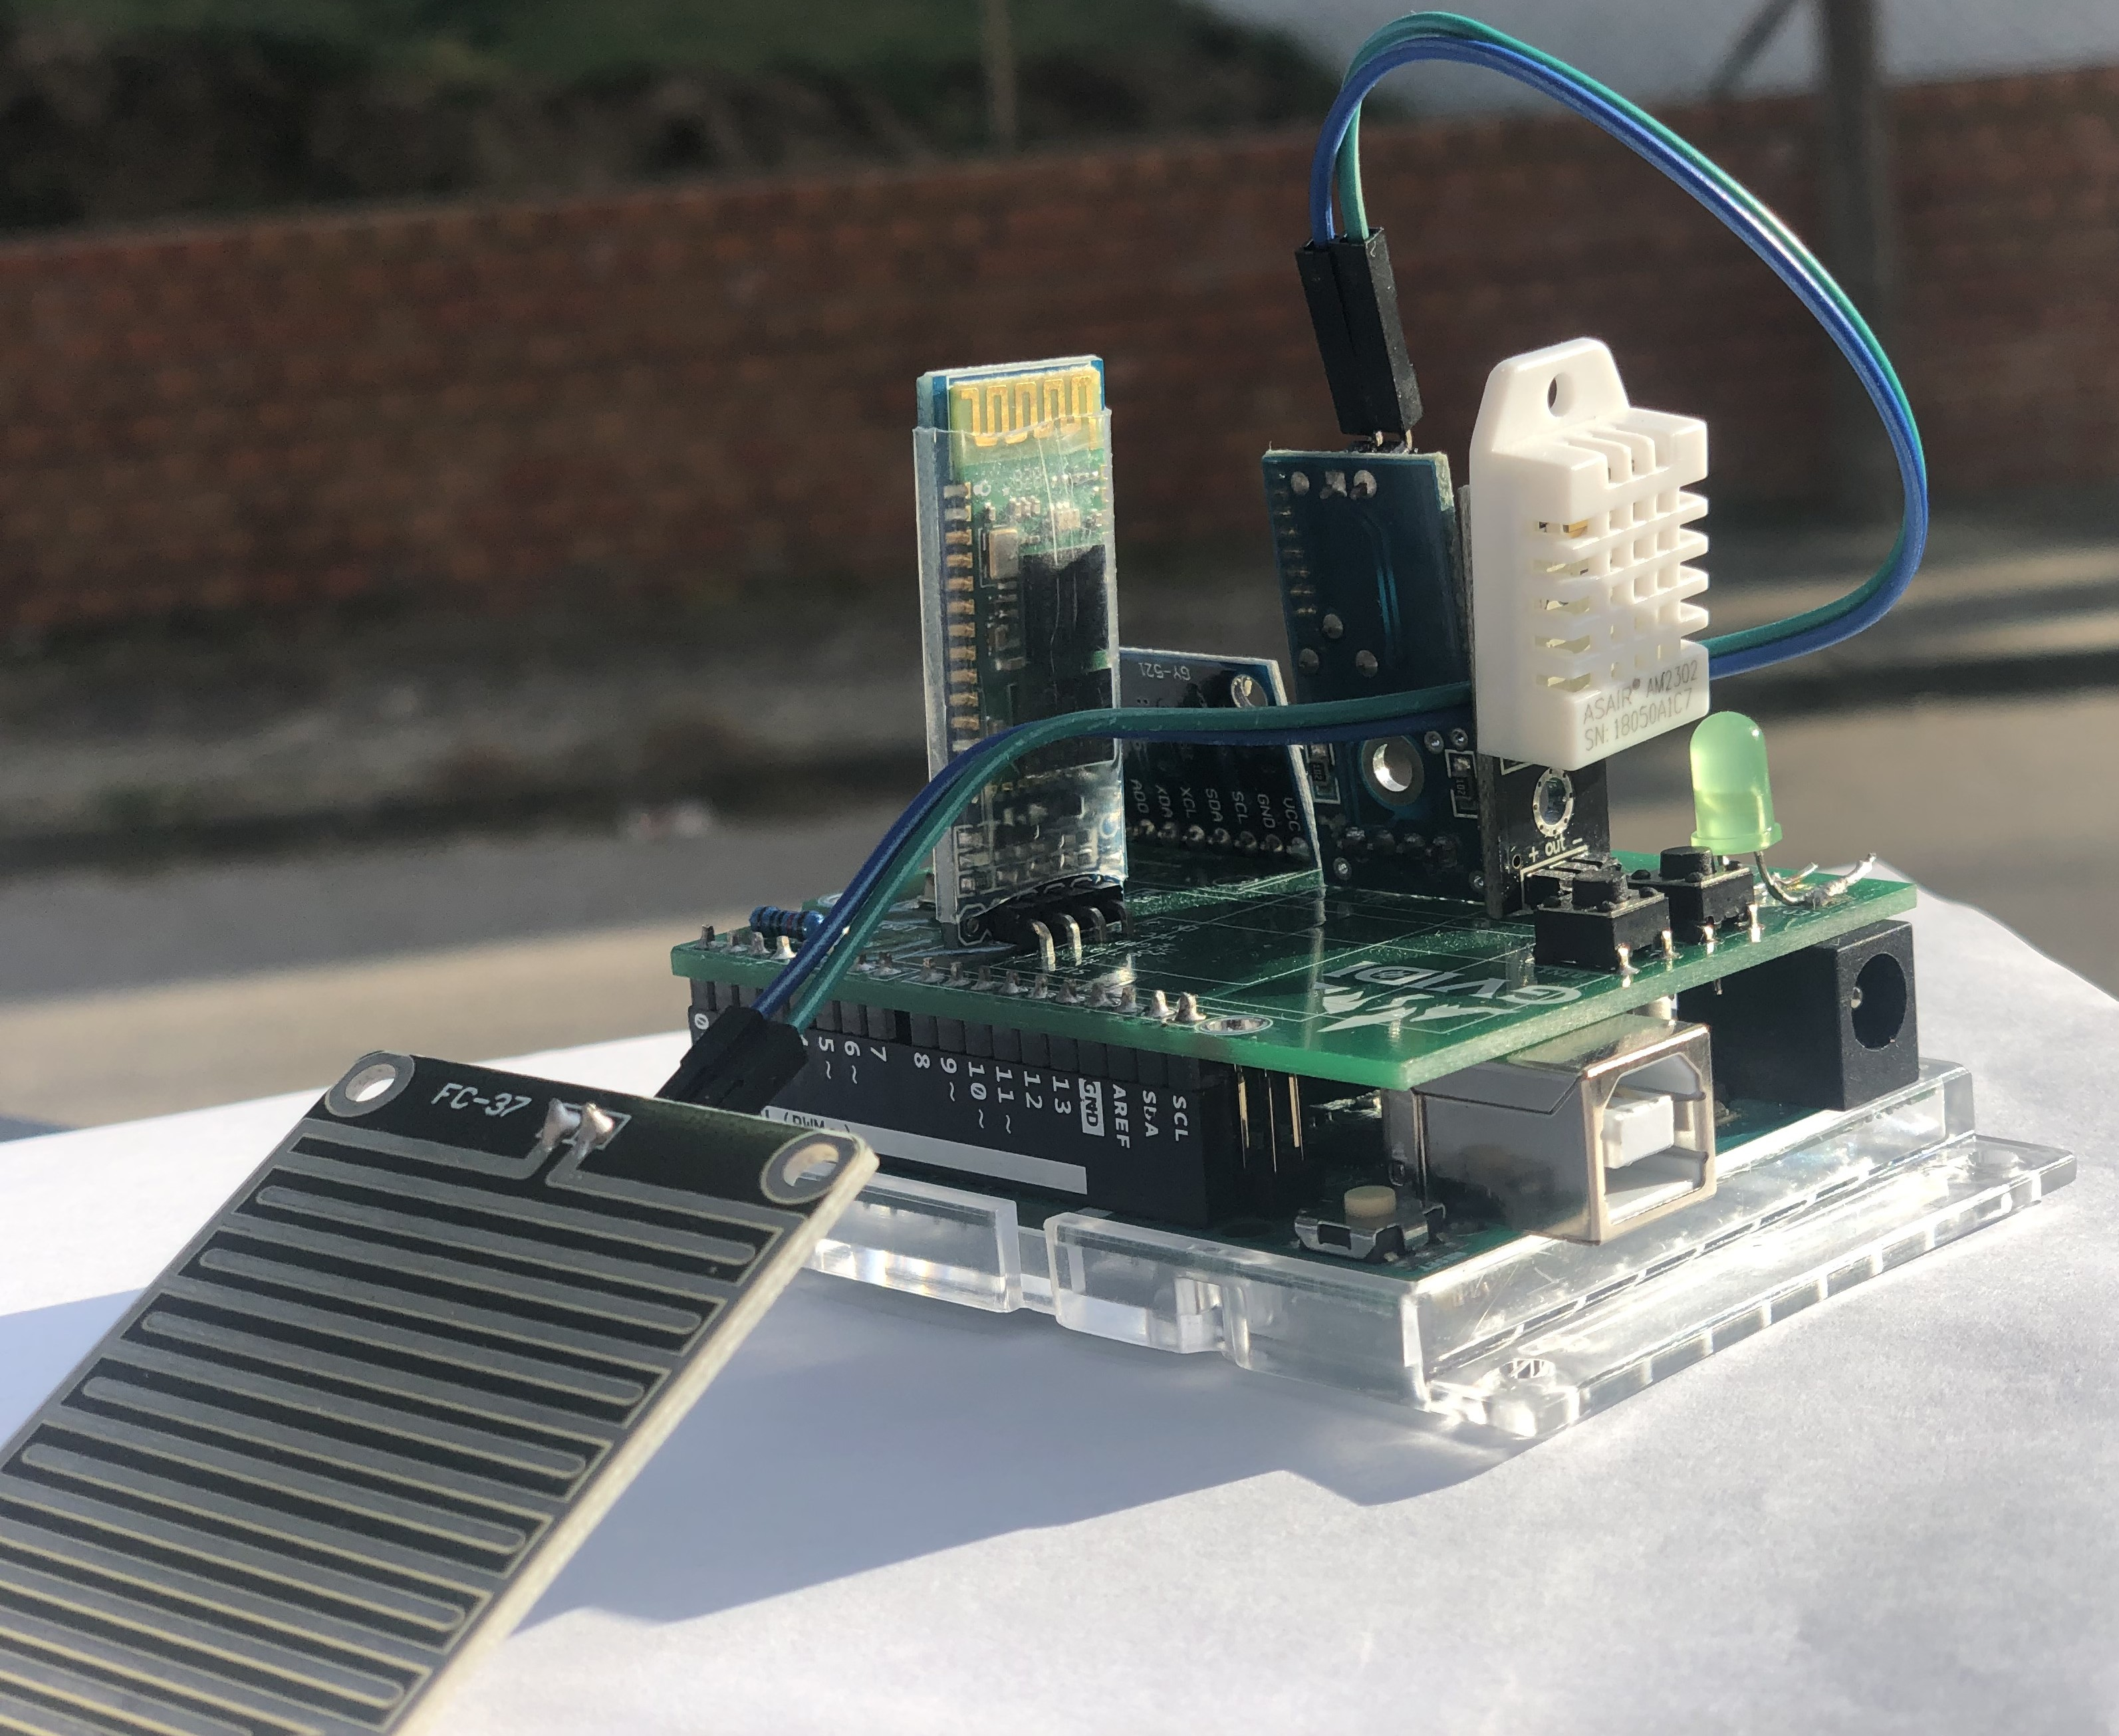
\includegraphics[width=0.5\textwidth]{prototype.jpg}
\caption{Prototipo final del microcontrolador conectado con todos los sensores que se usan.}
\label{fig:prototype}
\end{center}
\end{figure}

\section{Aplicación móvil}

En esta sección se va a mostrar en detalle tanto el diseño como la implementación de la aplicación móvil. La aplicación móvil se encarga del tratamiento, el análisis, el almacenamiento y la visualización de los datos captados por el dispositivo físico. Se trata de la parte más compleja del proyecto por lo que se expondrán distintas alternativas que se han barajado a lo largo del mismo, y el por qué se han tomado o descartado dichas alternativas. 

La aplicación móvil se ha implementado únicamente para el sistema operativo \textit{Android}, ya que no se disponía de tiempo físico ni de recursos para implementar la aplicación móvil en otros sistemas operativos como \textit{iOS}. Sin embargo esto no es un gran inconveniente ya que la mayoría de la población usa un dispositivo móvil \textit{Android} (en junio del año 2018 la venta de \textit{iPhones} suponía un total del $18.94\%$ de todos los dispositivos móviles vendidos).

\subsection{Diseño de la aplicación móvil}

Para el diseño de la aplicación móvil, en primer lugar, se realizaron bocetos de las distintas pantallas para tener una idea clara de la información relevante a mostrar. De esta forma la implementación se centra en conseguir la información que hay que mostrar y no se pierde tiempo implementando características que al final se desechan o que no son usadas. 

La aplicación móvil se ha diseñado siguiendo el patrón de arquitectura de \textit{software} \ac{MVC} o patrón Modelo-Vista-Controlador (véase Figura \ref{fig:mvc}). Este patrón permite realizar una separación entre la lógica de tratamiento de los datos, la interfaz de usuario y la lógica de control (o la lógica de aplicación).

\begin{itemize}
\item \textbf{Modelo}. Contiene la representación de los datos que gestiona el sistema y permite el acceso a sistemas de persistencia de datos, como pueden ser las bases de datos.
\item \textbf{Vista}. La vista se trata de la interfaz de usuario, es decir, la parte del sistema que permite al usuario interaccionar con el mismo de forma directa.
\item \textbf{Controlador}. Este elemento actúa como intermediario entre la vista y el modelo. Recibe las peticiones por parte del usuario, solicita los datos al modelo y una vez que los tiene, los envía a la vista para que el usuario pueda visualizarlos.
\end{itemize}

\begin{figure}[!h]
\begin{center}
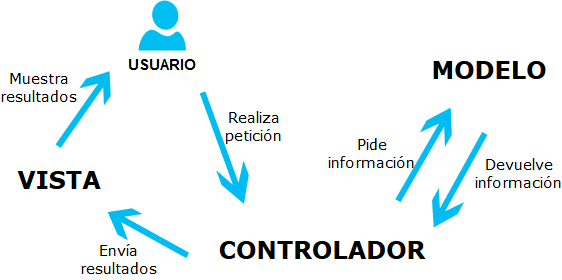
\includegraphics[width=0.5\textwidth]{mvc_arch.png}
\caption{Esquema general del patrón de arquitectura de \textit{software} \ac{MVC}.}
\label{fig:mvc}
\end{center}
\end{figure}

\subsection{Funcionalidad de la aplicación móvil}
\label{functionalityAppMovil}

Como se ha comentado anteriormente, la aplicación móvil se ha implementado para el sistema operativo \textit{Android}, usando \texttt{Java} como lenguaje de programación. La aplicación se compone de varias pantallas, siendo cada una de ellas una \textit{Activity}. Una \textit{Activity} en \textit{Android} es un componente que contiene una interfaz o una pantalla con la cual los usuarios pueden interaccionar. Las actividades que conforman la aplicación son las siguientes:

\begin{itemize}
\item \textbf{Actividad \textit{Signup}}. Esta actividad se utiliza tanto para que los usuarios puedan registrarse en la plataforma, como para que los usuarios que ya están registrados en la misma puedan acceder a ella. Como se puede ver en la Figura \ref{fig:signup}, tan solo es necesario un nombre de usuario, un correo electrónico y una contraseña para registrarse ya que dichos datos son los datos mínimos necesarios para realizar un registro en la plataforma.

\item \textbf{Actividad \textit{ResetPassword}}. Esta actividad se utiliza como medio de recuperación de la contraseña de un usuario, si este no la recuerda. Tan solo necesita proporcionar el correo electrónico con el que se registró en la plataforma y le serán enviadas a dicho correo las instrucciones para restablecer la contraseña.

\item \textbf{Actividad \textit{JoinExpedition}}. Esta actividad (ver Figura \ref{fig:newpass}}) tan solo es visible si el usuario que se ha autenticado en el sistema tiene el rol de participante. En ella se muestran en una lista los nombres de todas las expediciones que se encuentran en curso en el momento, junto con el correo electrónico del guía de la expedición. Cuando el participante selecciona una expedición de la lista, se une a ella de forma automática.

\item \textbf{Actividad \textit{CreateExpedition}}. Esta actividad tan solo es visible si el usuario que se ha autenticado en el sistema tiene el rol de guía. Gracias a la misma, los guías podrán crear nuevas expediciones de manera muy sencilla, indicando tan sólo el nombre de la expedición (como se puede ver en la Figura \ref{fig:createExp}).

\item \textbf{Actividad \textit{ExpeditionDetails}}. Esta actividad tan solo es visible si el usuario que se ha autenticado en el sistema tiene el rol de guía. En esta actividad los guías pueden ver detalles generales de la expedición como las alertas generadas en una franja de tiempo, los participantes que se encuentran a más de un cierto umbral de distancia, el número de participantes que han solicitado una parada desde la última parada realizada y el número de participantes que tienen menos de un cierto nivel de batería en sus terminales. En definitiva, gracias a esta actividad el guía puede tener una vista general de la expedición de una forma rápida.

\item \textbf{Actividad \textit{ParticipantDetails}}. Al igual que las dos actividades anteriores, esta actividad es solo visible para el rol de guía. Esta actividad (ver Figura \ref{fig:extpar}) se muestra cuando el guía selecciona un determinado participante en el mapa de la vista principal y en ella se puede ver toda la información acerca del participante. Entre esta información destacan todas las alertas que ha generado el participante, su ritmo (tanto actual como el ritmo medio) y el nivel de batería que tiene el dispositivo móvil del participante.

\item \textbf{Actividad principal}. Esta actividad es compartida tanto por los participantes como por los guías y muestra la información relevante para los usuarios (tanto participantes como guías) mientras la expedición está en curso. En esta vista podemos destacar el mapa en el cual se pueden visualizar todos los usuarios de la expedición. El guía se muestra en color azul y los participantes aparecerán en color verde, amarillo o rojo dependiendo de la distancia con respecto al guía.

\begin{figure}
 \centering
  \subfloat[Vista de \textit{Login}]{
   \label{fig:signin}
    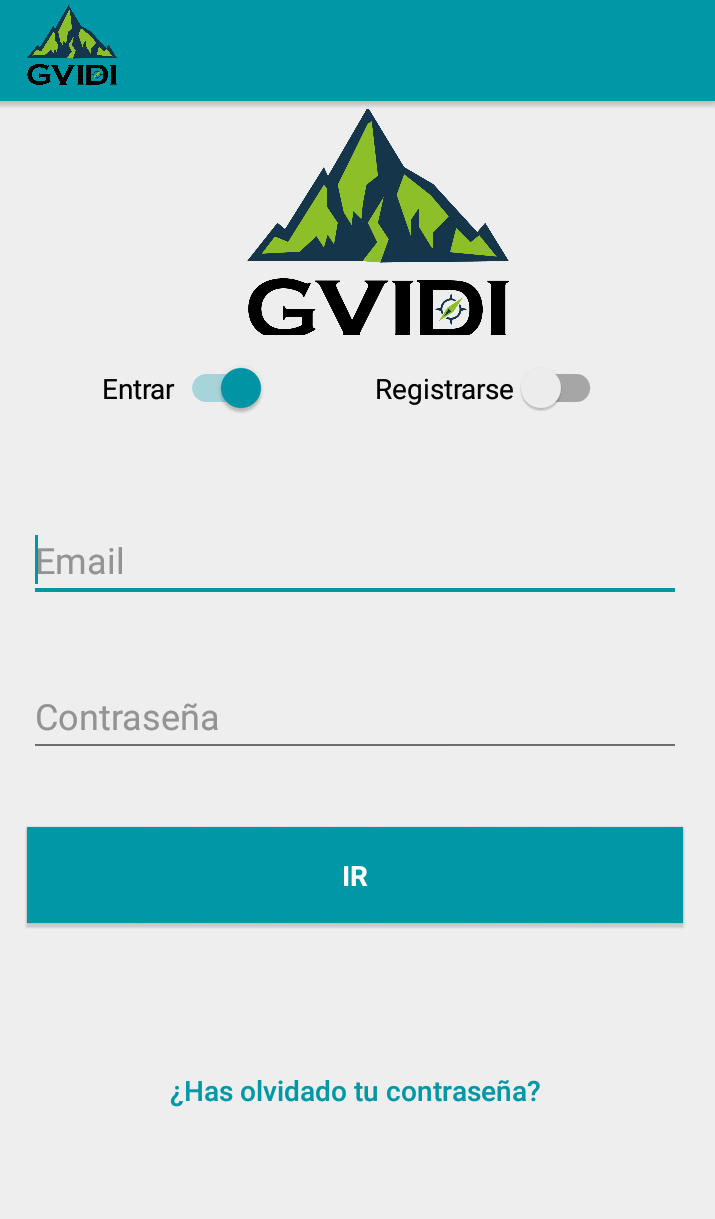
\includegraphics[width=0.3\textwidth]{login.png}}
  \subfloat[Vista de registro.]{
   \label{fig:signup}
    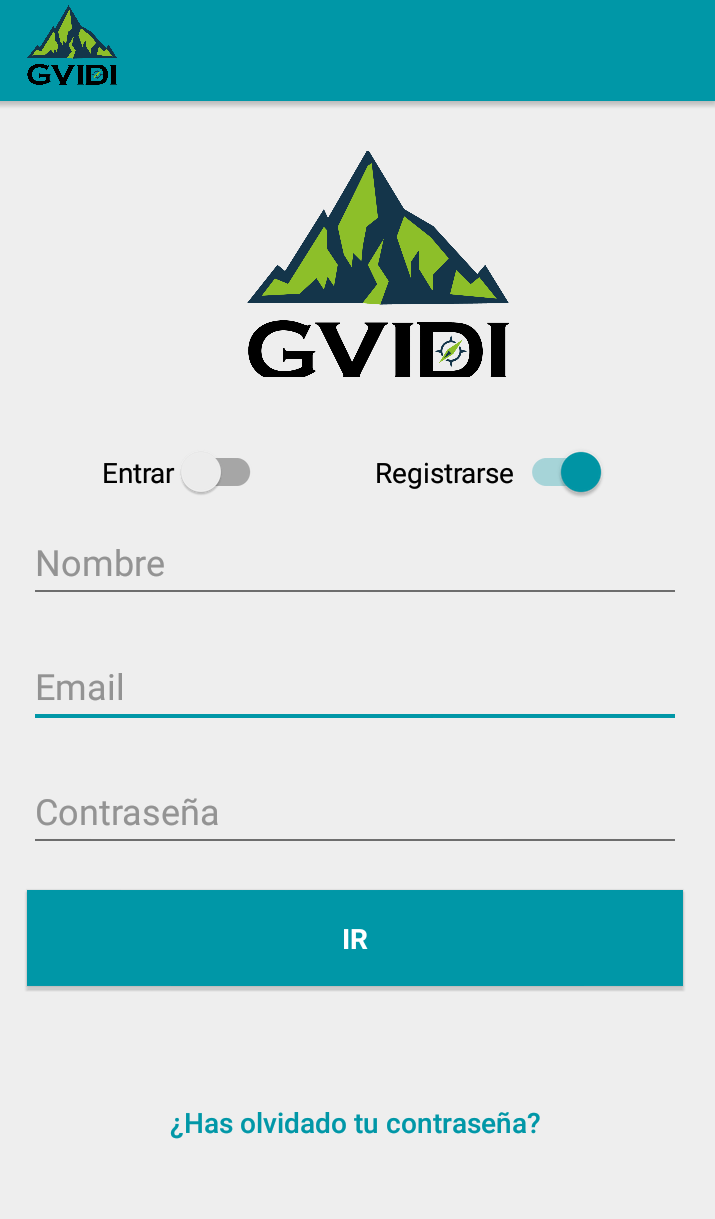
\includegraphics[width=0.3\textwidth]{signin.png}}
  \subfloat[Vista de la actividad para reestablecer la contraseña.]{
   \label{fig:newpass}
    
\includegraphics[width=0.3\textwidth]{newpass.png}}
    
  \caption{Pantallas de inicio de sesión, registro y reestablecimiento de contraseña.}
  \label{fig:fig1}
\end{figure}

\begin{figure}
 \centering
  \subfloat[Vista de la actividad para unirse a expediciones en curso.]{
   \label{fig:join}
    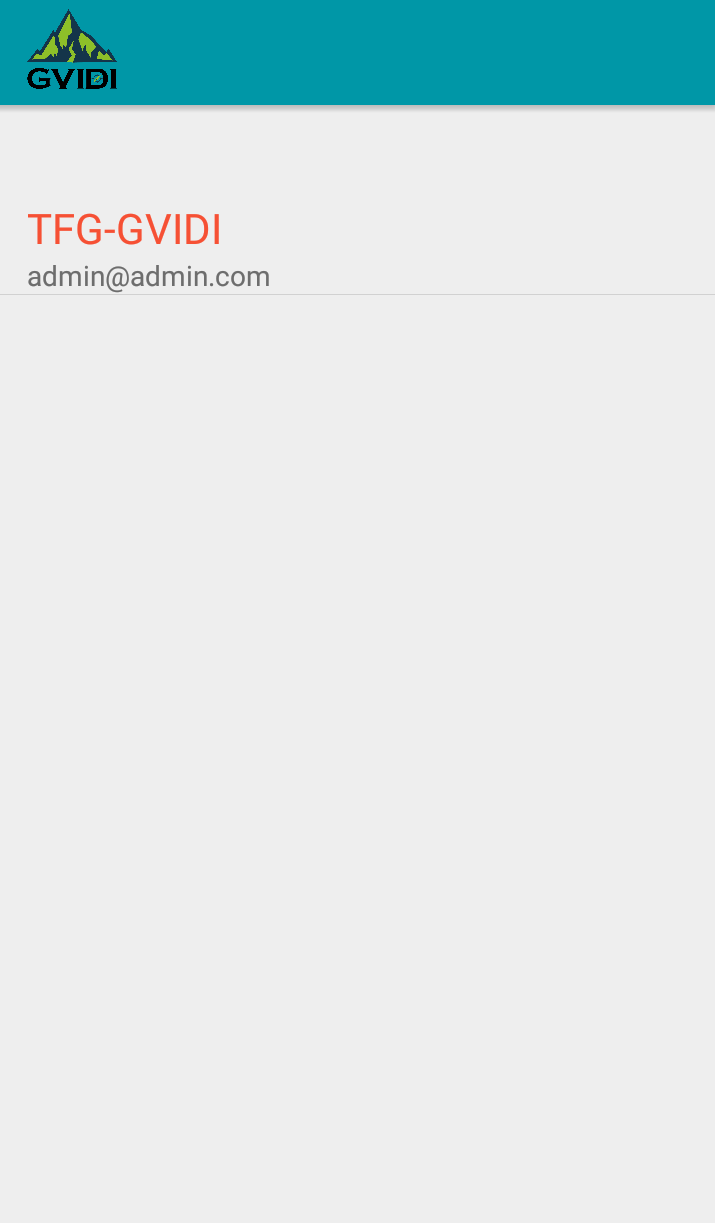
\includegraphics[width=0.3\textwidth]{join.png}}
  \subfloat[Vista de la actividad para crear una nueva expedición.]{
   \label{fig:createExp}
    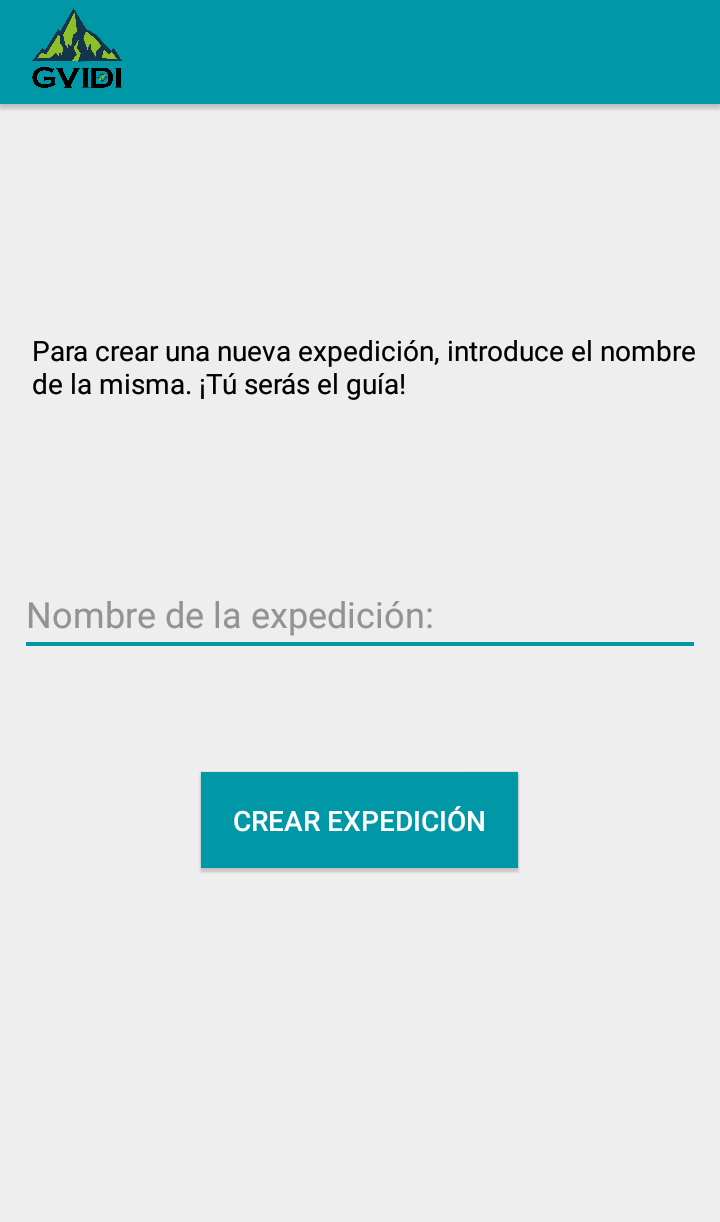
\includegraphics[width=0.3\textwidth]{createExp.png}}
  \subfloat[Vista parcial de la actividad para visualizar el estado general de la expedición.]{
   \label{fig:extexp}
    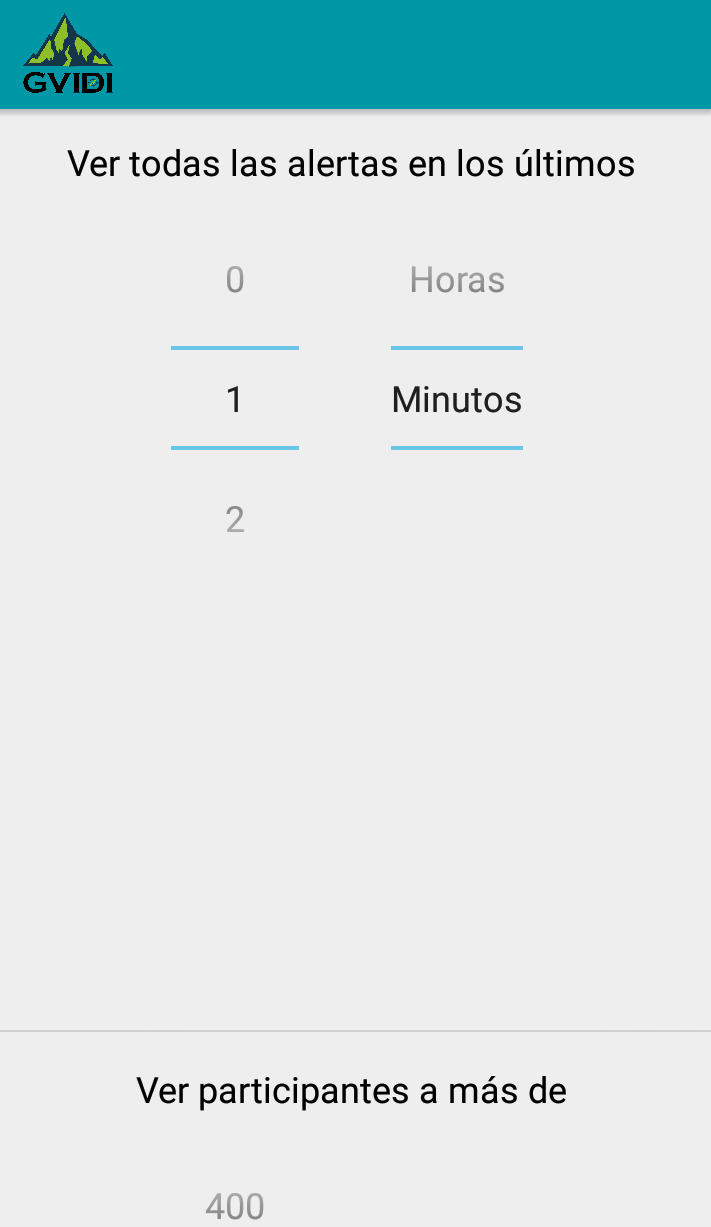
\includegraphics[width=0.3\textwidth]{extexp.png}}
  
  \caption{Pantallas de unión a expedición en curso, creación de expedición y vista del estado general de la expedición.}
  \label{fig:fig2}
\end{figure}

\begin{figure}
 \centering
  \subfloat[Vista de la actividad de detalles de un participante.]{
   \label{fig:extpar}
    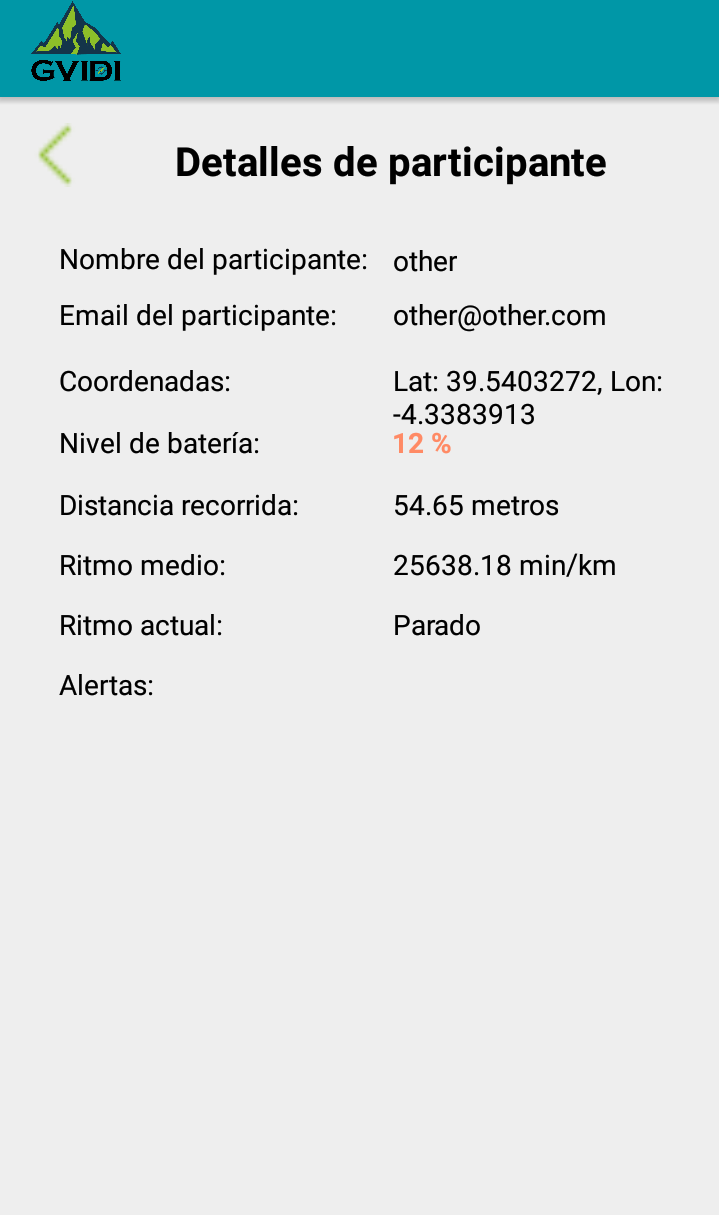
\includegraphics[width=0.3\textwidth]{extpar.png}}
  \subfloat[Vista de la actividad principal.]{
   \label{fig:main}
    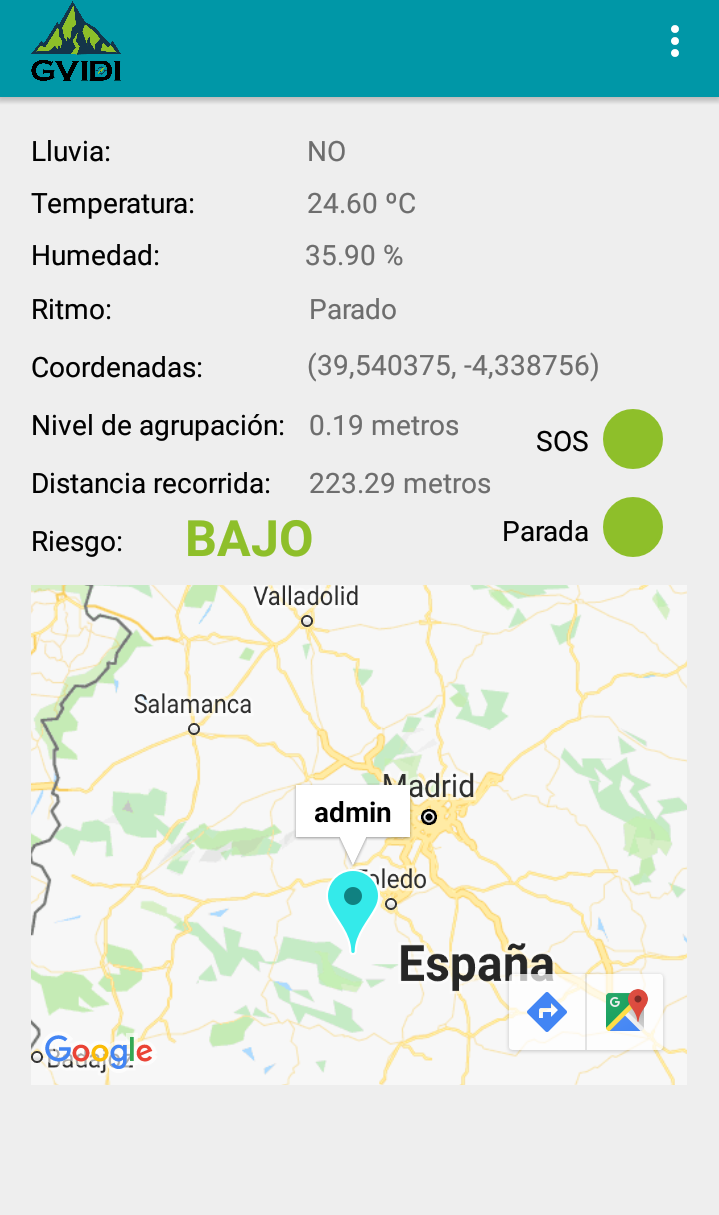
\includegraphics[width=0.3\textwidth]{main.png}}
  \caption{Pantalla de vista en detalle de un participante y pantalla principal.}
  \label{fig:fig3}
\end{figure}

\end{itemize}

\subsection{Comunicación entre la aplicación móvil y el dispositivo físico}

Como se ha mencionado en numerosas ocasiones anteriormente, los datos que envía el microcontrolador provenientes de los sensores que lleva equipados son enviados al dispositivo móvil a través de \textit{Bluetooh}. Por esto es necesario que la aplicación móvil pueda dar soporte a esta comunicación, y para ello se ha implementado la solución que se puede observar en la Figura \ref{fig:arqu_blue}.

\begin{figure}[!h]
\begin{center}
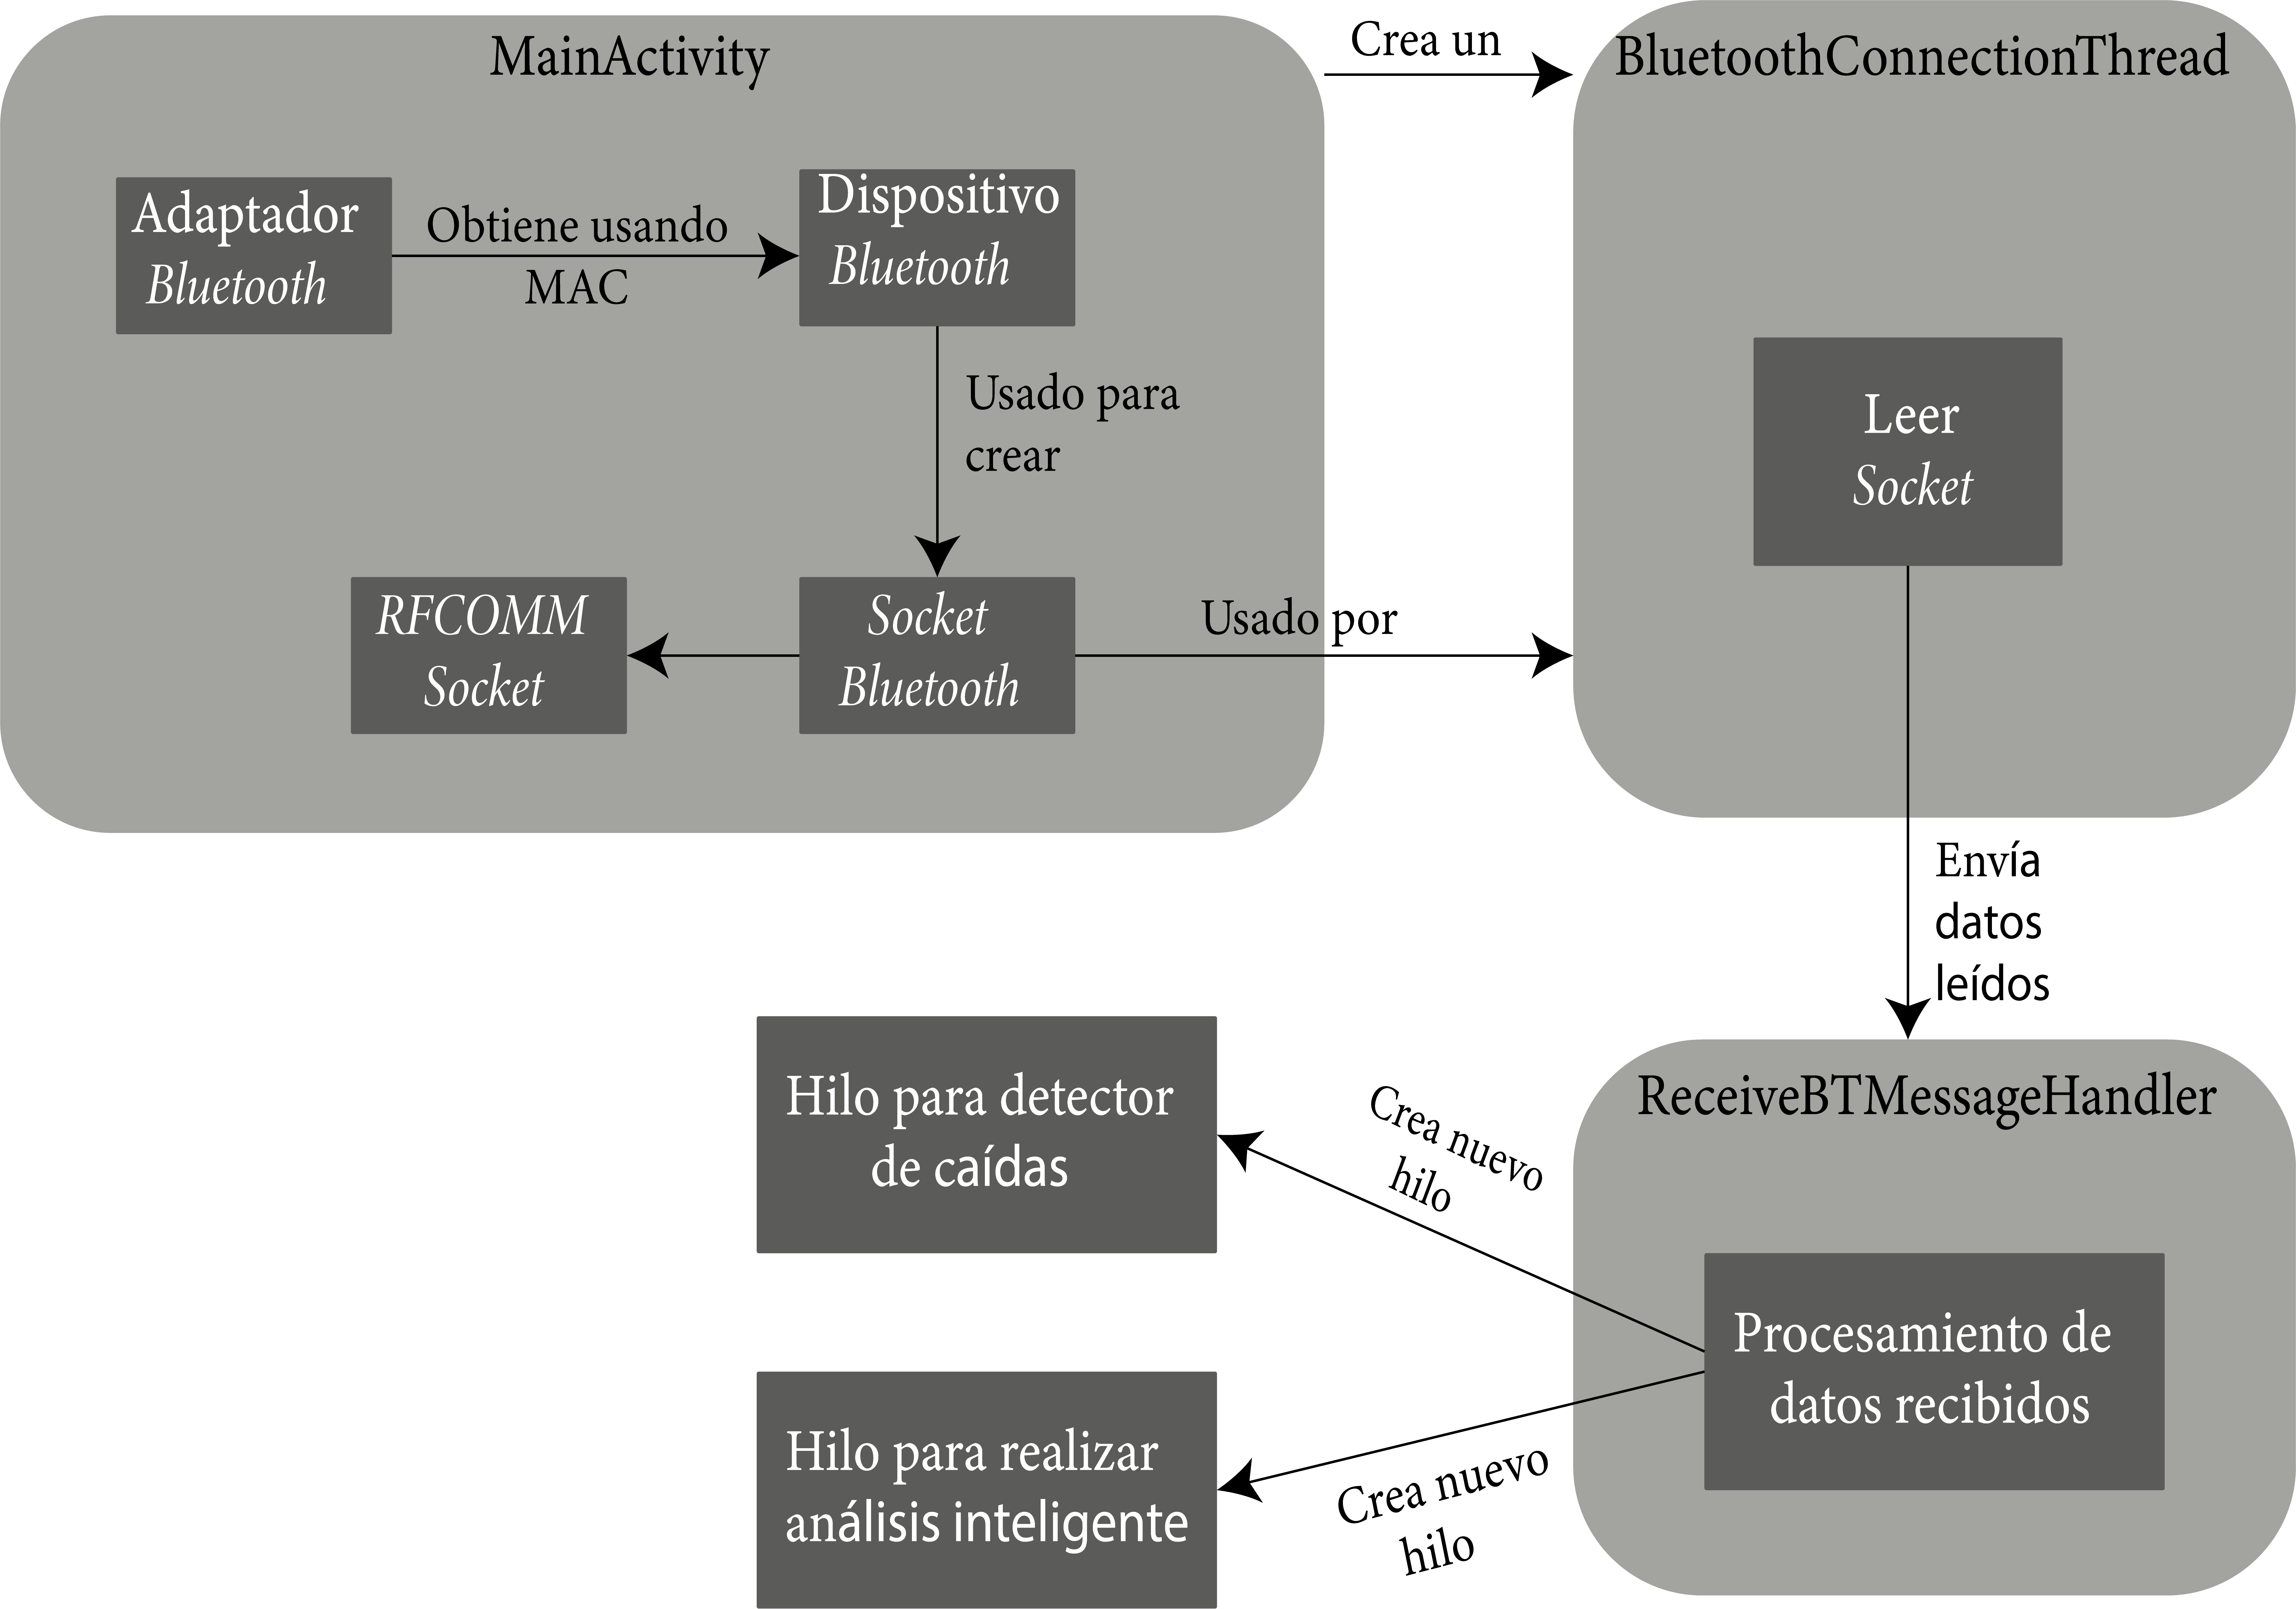
\includegraphics[width=0.8\textwidth]{arquitectura_bluetooth.png}
\caption{Arquitectura de la comunicación \textit{Bluetooth} en el dispositivo móvil.}
\label{fig:arqu_blue}
\end{center}
\end{figure}

Para poder realizar una conexión usando el protocolo inalámbrico \textit{Bluetooth} es necesario realizar una conexión usando \textit{sockets} \ac{RFCOMM}. Para crear un \textit{socket} siempre es necesario proporcionar una tupla compuesta por una dirección y un número de puerto (como ocurre por ejemplo con los \textit{sockets} \texttt{TCP/IP}). En los \textit{sockets} \ac{RFCOMM}, la dirección que hay que proporcionar al \textit{socket} es la dirección \ac{MAC} del dispositivo \textit{bluetooth} con el que se quiere realizar la conexión. En este proyecto, no se usa un puerto específicamente definido y el número de puerto se gestiona de forma automática. 

Para obtener la dirección \ac{MAC} del dispositivo con el que se realizará la conexión \textit{Bluetooth} es necesario realizar una búsqueda de dispositivos. En este proyecto, la \ac{MAC} se obtiene realizando una búsqueda de dispositivos \textit{Bluetooth} en los dispositivos que han sido emparejados con el teléfono móvil (ver Listado \ref{lst:getMAC}). Una vez que se han recuperado los dispositivos emparejados se muestran al usuario para que pueda elegir el dispositivo \textit{Bluetooth} con el que quiere realizar la conexión. Si esta conexión es fallida (porque el dispositivo que elige está fuera del alcance o no se encuentra disponible en ese momento) el usuario tendrá que volver a elegir el dispositivo con el que se conectará.

\begin{lstlisting}[language=java,captionpos=t,caption={\textbf{Búsqueda de dispositivos \textit{Bluetooth} emparejados para obtener la dirección \ac{MAC}.}},label={lst:getMAC}]
if (btAdapter.isEnabled() && macAddress == null) {
  // Buscar dispositivos emparejados
  Set<BluetoothDevice> pairedDevices = btAdapter.getBondedDevices();
  if (pairedDevices.size() > 0) {
    // Mostrar al usuario los dispositivos emparejados para que elija con el que 
    // se quiere conectar  
  }
}
\end{lstlisting}

Cuando se recupera el dispositivo \textit{Bluetooth} con el que se va a realizar la conexión, se puede crear el \textit{socket Bluetooth} que se ha comentado anteriormente, usando la dirección \ac{MAC} del dispositivo recuperado. Si el \textit{socket} se crea y se conecta con el dispositivo remoto de forma satisfactoria, se puede proceder a la recepción o envío de datos por medio de este \textit{socket}. En este proyecto el dispositivo móvil sólo recibe los datos provenientes del microcontrolador y no envía nada a este último. 

Para la recepción de datos, se ha creado un nuevo hilo, ya que el hilo principal de la aplicación se encarga de mostrar la información al usuario en la pantalla del teléfono y si la recepción de datos se realiza en este hilo, se bloqueará y el usuario no podrá usar la aplicación porque esta se encontrará ``bloqueada'' recibiendo los datos por \textit{Bluetooth}. El nuevo hilo estará recibiendo los datos que llegan por el \textit{socket Bluetooth} de forma continua.

Como es necesario que se reciban la mayor cantidad de datos posibles en un cierto periodo de tiempo (así lo requiere el algoritmo para detectar caídas, como se comentará más adelante), el código del hilo que lee los datos del \textit{socket} debe ser lo más reducido posible, así leerá datos del \textit{socket} más rápidamente. El cometido del hilo tan sólo es leer desde el \textit{socket} y enviar los datos leídos a un manejador que los procesará mas a fondo (véase Listado \ref{lst:btthread}).

\begin{lstlisting}[language=java,captionpos=t,caption={\textbf{Hilo secundario que lee datos del \textit{socket Bluetooth} y los envía a un manejador.}},label={lst:btthread}]
while (true) {
  try {
    number_of_incoming_bytes = input_bytes.read(buffer);
    // Notificar al manejador ReceiveBTMessageHandler del nuevo mensaje que se recibe
    handler.obtainMessage(1, number_of_incoming_bytes, -1, buffer).sendToTarget();
  } catch (IOException e) {
    break;
  }
}
\end{lstlisting}

Cuando el manejador de mensajes recibe los datos que se han leído del \textit{socket}, se crean dos nuevos hilos, uno que se encargará del algoritmo para detectar caídas y otro que se encargará del resto del análisis inteligente (análisis del riesgo de caída en la expedición y análisis de distancias). Se crean dos hilos debido, principalmente, a que el algoritmo del detector de caídas necesita nuevos datos de aceleración (provenientes del acelerómetro instalado en el microcontrolador) lo más rápidamente posible y con la creación de un nuevo hilo cada vez que se leen nuevos datos del \textit{socket Bluetooth} dedicado únicamente a proporcionar datos de aceleración al algoritmo de detección de caídas se consigue la máxima eficiencia de dicho algoritmo. 

Merece la pena comentar que la creación de nuevos hilos cada vez que se leen nuevos datos del \textit{socket} no proporciona solo ventajas, sino también inconvenientes a tener muy en cuenta. La funcionalidad para la detección de caídas se encuentra dentro de una clase que sigue un patrón \textit{singleton} (todo esto se comentará en detalle más adelante), por lo que solo existe una instancia de esta clase. Todos los hilos que se crean comparten la misma instancia y, por tanto, hay que ser muy cuidadosos al acceder a propiedades de dicha clase cuando se quiere escribir en ellas. Identificar las secciones críticas y protegerlas con mecanismos de sincronización como los semáforos \textit{mutex} es esencial en este caso.

\subsubsection{Problemas encontrados y sus soluciones en la comunicación por \textit{Bluetooth}.}

\\

En este apartado se van a comentar los problemas más importantes que se han presentado durante la implementación de la conexión del dispositivo móvil con el módulo de \textit{Bluetooth} del microcontrolador, así como las soluciones implementadas para resolver dichos problemas.

En una primera implementación, se crearon dos \textit{sockets} para realizar la conexión por \textit{Bluetooth}. Uno de los \textit{sockets} sería usado cuando la aplicación estaba en uso de forma normal y el otro \textit{socket} se usaría para seguir recibiendo datos en segundo plano, cuando la aplicación no se encuentra activa o se producen cambios de pantalla. Cada uno de los \textit{sockets} se creaba usando un puerto distinto y sólo uno de los \textit{sockets} estaría conectado a la vez. Cuando la aplicación se iniciaba, se creaba y conectaba un \textit{socket} de forma normal. Cuando la actividad era destruida (bien por un cambio de actividad o bien por salir de la aplicación), el \textit{socket} conectado debía desconectarse para dar paso al \textit{socket} que era usado en segundo plano. Sin embargo, a partir de esa primera desconexión, los \textit{sockets} no se conectaban con éxito más y se dejaban de recibir datos.

\begin{figure}[!h]
\begin{center}
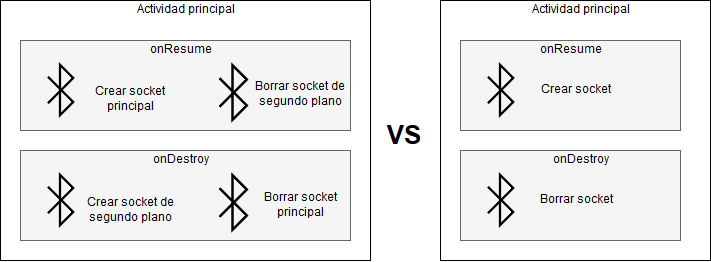
\includegraphics[width=0.7\textwidth]{problemBT.png}
\caption{Problema en el uso de dos \textit{sockets Bluetooth} y su solución.}
\label{fig:problemBT}
\end{center}
\end{figure}

Para resolver ese problema, se ha optado por usar tan solo un \textit{socket Bluetooth}, que es creado en el método \texttt{onResume} de la actividad principal (es decir, cuando la actividad es creada) y que es destruido en el método \texttt{onDestroy}. De esta forma, aunque no se puedan recibir datos en segundo plano, los \textit{sockets} se crean y se conectan al dispositivo remoto de forma correcta.

El último problema a destacar en la comunicación por \textit{Bluetooth} es que en un principio todo el análisis inteligente era realizado por el manejador creado por el hilo secundario (el hilo que trata las lecturas del \textit{socket Bluetooh}). Este manejador se encargaba tanto de realizar el algoritmo de detección de caídas, como del análisis del riesgo de caída en la expedición y el análisis de distancias de los participantes con respecto al guía de la misma. Esto daba como resultado que se leían datos del \textit{socket} algo menos de una vez por segundo, claramente insuficiente para el algoritmo de detección de caídas. Una frecuencia de lectura del \textit{socket} tan baja significa que muchos datos de aceleración del usuario no eran leídos (como se comentará más adelante la detección de caídas está motivada por la superación de unos ciertos umbrales por parte de los valores de aceleración. Si no se realiza la lectura del valor de aceleración que supera esos umbrales, no será posible detectar una caída) por lo que las caídas no se inferían correctamente.

Para resolver este problema, se ha hecho uso de la solución comentada anteriormente. Cada vez que se realiza una lectura del \textit{socket}, se crean dos hilos alternativos (uno que se encarga de la detección de caídas y otro que se encarga del resto del análisis inteligente). De esta forma, se ha logrado multiplicar por cuatro la frecuencia de lectura del \textit{socket}, ya que ahora se realizan unas cuatro lecturas por segundo. Esto ha permitido que la detección de caídas sea mucho más precisa ya que es más difícil que la información asociada a una caída (un determinado valor de aceleración que supera unos ciertos umbrales establecidos) no sea leída (aún así, el algoritmo de detección de caídas también contempla la pérdida de información crítica puntual, como se comentará más adelante).

\subsection{Autenticación de usuarios en \texttt{Firebase} y almacenamiento de datos en \texttt{Firestore}} 

\texttt{Firebase} es una plataforma para aplicaciones (tanto \textit{webs} como móviles) que está integrada dentro de la nube de \texttt{Google} y proporciona, entre otros, un servicio de autenticación de usuarios (\textit{Firebase Auth}) usando únicamente código en el lado del cliente. En este proyecto se ha decidido usar \texttt{Firebase} para homogeneizar la autenticación de usuarios tanto en la plataforma \textit{web} realizada como en la aplicación móvil, evitando reescribir código de acceso a un sistema de almacenamiento de usuarios propio a medida en dos lenguajes distintos (\texttt{Java} en la aplicación móvil y \texttt{Javascript} en el \textit{backend} de la plataforma \textit{web}).

Además, cabe destacar que \texttt{Firebase Auth} proporciona un sistema de autenticación altamente usado y probado por lo que la seguridad en la autenticación es mayor que usando un sistema de autenticación propio. La seguridad en la autenticación es crítica, ya que de ella dependen los datos del usuario que usa la aplicación.

Hay que tener en cuenta que, de acuerdo a la \ac{LOPD}, los datos se recogen de manera lícita, leal y transparente. En este proyecto, el usuario está al tanto de todos los datos que se recogen y los acepta para su monitorización (por lo que los datos tienen un fin legítimo y explícito). No se recogen más datos de los estrictamente necesarios y tampoco se recogen datos de los que el usuario no es consciente. Una de las razones principales por las que se ha usado tanto \texttt{Firebase}, como \texttt{Firestore}, es que la \ac{LOPD} exige que los datos personales sean tratados con la adecuada seguridad (y estas plataformas lo cumplen).

Para poder usar \texttt{Firebase} en este proyecto, ha sido necesario crear un nuevo proyecto en la \textit{web} de \texttt{Firebase} (\url{https://console.firebase.google.com}). Para ello solo es necesario indicar un nombre de proyecto y una vez creado, añadir al mismo una aplicación \textit{Android} que en este caso es la aplicación que se ha desarrollado. En la Figura \ref{fig:fireauth} se puede observar la información de la aplicación \textit{Android}, que será necesario incluir en la misma para poder realizar conexiones con la \ac{API} de \texttt{Firebase}.	

\begin{lstlisting}[language=java,captionpos=t,caption={\textbf{Inicio de sesión usando \texttt{Firabase Auth}.}},label={lst:firebaseauth}]
FirebaseAuth auth = FirebaseAuth.getInstance();
auth.signInWithEmailAndPassword(email, password).addOnCompleteListener(
  SignupActivity.this, new OnCompleteListener<AuthResult>() {
    @Override
    public void onComplete(@NonNull Task<AuthResult> task) {
      if (task.isSuccessful()) {
        startActivity(new Intent(SignupActivity.this, MainActivity.class));
        finish();
      } else {
        Toast.makeText(SignupActivity.this, "Authentication has failed", Toast.LENGTH_SHORT).show();
      }
    }
  }
);
\end{lstlisting}

\begin{figure}[!h]
\begin{center}
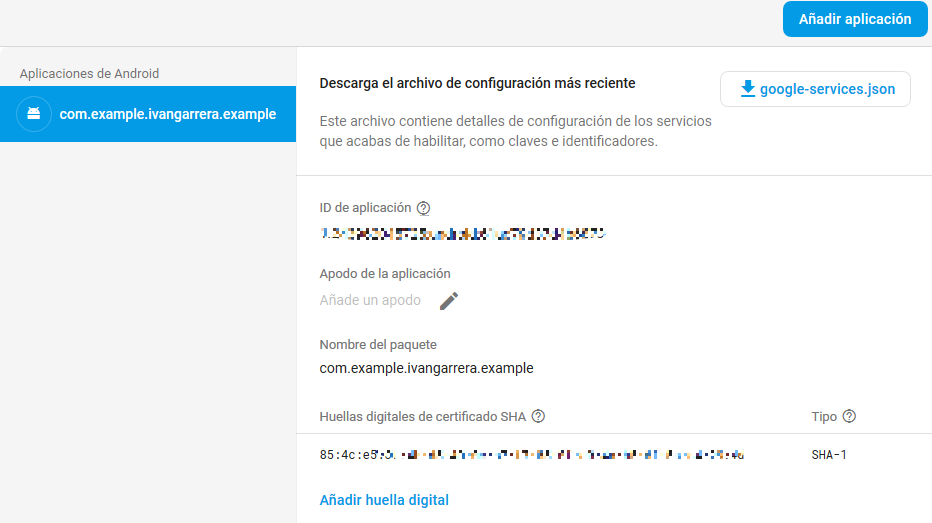
\includegraphics[width=0.8\textwidth]{fireauth.png}
\caption{Credenciales necesarias para poder acceder a la \ac{API} de \texttt{Firebase} en la aplicación \textit{Android}.}
\label{fig:fireauth}
\end{center}
\end{figure}

En el Listado \ref{lst:firebaseauth} se puede observar la facilidad en el inicio de sesión, usando \texttt{Firebase Auth}. Todas las llamadas a la \ac{API} de \texttt{Firebase} son llamadas asíncronas, es decir, no bloquean el hilo que realiza la llamada hasta que no terminan su trabajo. En este caso, se procede a realizar la autenticación de forma asíncrona (por lo que mientras la autenticación no se completa, el programa seguirá ejecutando las siguientes instrucciones) y el código del método \texttt{onComplete} se ejecutará cuando se haya completado la autenticación. Dentro de este \textit{callback} se encontrará la lógica que decide qué hacer si la autenticación ha tenido éxito o qué hacer si no lo ha tenido.

\texttt{Firestore} es una base de datos de documentos \texttt{NoSQL} rápida, completamente administrada, sin servidor y que ofrece servicios \textit{cloud} para almacenar, sincronizar y consultar datos desde aplicaciones tanto móviles como \textit{web}. Para hacer uso de \texttt{Firestore}, no se necesita un servidor intermedio que gestione el acceso a los datos, sino que se usa a través de llamadas a una \ac{API} definida. Los datos se consultan y envían a \texttt{Firestore} serializados en \ac{JSON}. 

En el Listado \ref{lst:firestoredata} se puede observar el formato de los datos que proporciona la aplicación móvil y se almacenan en \texttt{Firestore}. Estos datos pertenecen a una expedición, que como se puede observar está formada por un guía y una serie de participantes. La información que almacena cada participante es exactamente la misma que la que almacena el guía. Como se puede ver, toda la información almacenada es la necesaria para llevar a cabo los objetivos del proyecto.

\begin{lstlisting}[language=json,captionpos=t,caption={\textbf{Formato de los datos almacenados en \texttt{Firestore} para una expedición.}},label={lst:firestoredata}]
{
  "Duration": int,
  "EndTime": long,
  "ExpName": string,
  "Guide": {
    "Alerts": [],
    "BatteryLevel": int,
    "Humidity": [],
    "Lat": string,
    "Lon": string,
    "PreviousLocations": [
      {
        "Lat": string,
        "Lon": string,
        "Timestamp": long
      }
    ],
    "Temperature": [],
    "TotalDistance": double,
    "id": string
  },
  "InProgress": boolean,
  "InitTime": long,
  "LastStop": long,
  "Participants": []
}
\end{lstlisting}

Como se puede ver en el Listado \ref{lst:firestorecode}, la obtención de datos desde la base de datos \textit{cloud} de \texttt{Firestore} se realiza a través de llamadas a la \ac{API} asíncronas (al igual que ocurría con \texttt{Firestore}). El método \texttt{onComplete} será invocado cuando los datos que se han solicitado estén listos para su uso. Mientras esto no ocurra, la aplicación seguirá ejecutándose de manera normal. El uso de llamadas asíncronas aumenta el rendimiento de la aplicación, puesto que no hay que esperar sin poder ejecutar más código hasta que las llamadas completen su trabajo. Sin embargo, hay que tener en cuenta que los datos que devuelve la llamada a un método asíncrono podrían no estar disponibles cuando se requieren en el código más adelante (en el caso de que sean requeridos).

\begin{lstlisting}[language=java,captionpos=t,caption={\textbf{Obtención de todos los participantes de una determinada expedición.}},label={lst:firestorecode}]
DocumentReference documentReference = database.collection(DATABASE_NAME).document(expedition_name);
documentReference.get().addOnCompleteListener(new OnCompleteListener<DocumentSnapshot>() {
  @Override
  public void onComplete(@NonNull Task<DocumentSnapshot> task) {
    if (task.isSuccessful()) {
      Map<String, Object> expedition = task.getResult().getData();
      ArrayList<Map<String, Object>> participants =
               (ArrayList<Map<String, Object>>) expedition.get("Participants");

    }
  }
});
\end{lstlisting}

En la Figura \ref{fig:firebaseSequence} se puede observar un diagrama de secuencia que resume cómo se realizan en este proyecto las llamadas a la \ac{API} de \texttt{Firestore}. Las llamadas son iniciadas por el usuario en la vista, de forma directa (si pulsa un botón que devuelva las alertas de un participante, por ejemplo) o de forma indirecta (cuando se carga una actividad se cargan de forma automática ciertos datos que se solicitan a la base de datos) y, a través del controlador, se solicitan los datos al modelo. El modelo se encarga de solicitar los datos a \texttt{Firestore} y cuando son devueltos, los transforma al formato necesario. 

\begin{figure}[!h]
\begin{center}
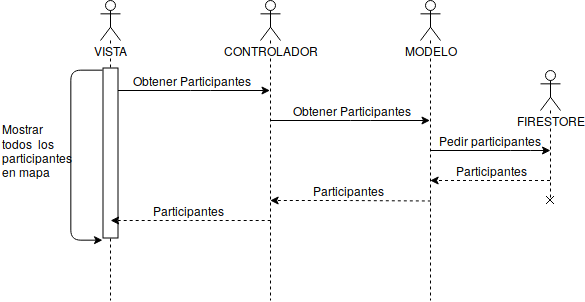
\includegraphics[width=0.8\textwidth]{firebaseSequence.png}
\caption{Diagrama de secuencia en llamadas a la base de datos en \texttt{Firestore}.}
\label{fig:firebaseSequence}
\end{center}
\end{figure}

\section{Detección automática de situaciones anómalas}

Como se ha explicado anteriormente la mayoría de los datos son recogidos a través de los sensores equipados en el microcontrolador y enviados al dipositivo móvil a través de \textit{Bluetooth}. Sin embargo, otros datos como los de posición, los toma el dispositivo móvil (véase Listado \ref{lst:location}). El dispositivo móvil se encarga de realizar este análisis inteligente.

Los datos que llegan a través de \textit{Bluetooth} tienen que ser sometidos a un \textbf{proceso de depuración}, antes de que puedan ser utilizados por los algoritmos de análisis inteligente. El proceso de depuración de datos es necesario porque en ocasiones se pueden leer datos del \textit{socket Bluetooth} incompletos o que están corruptos. Los datos que se envían por \textit{Bluetooth} desde el microcontrolador siguen la estructura que se puede observar en la Figura \ref{fig:datosBT}, por lo que cuando son recibidos en la aplicación móvil hay que asegurarse de que siguen esa misma estructura. Si cuando se realiza el proceso de depuración de datos, el mensaje no es correcto (bien porque no tenga el formato adecuado o bien porque los datos se hayan corrompido) se desecha por completo el mensaje ya que inferir por \textit{software} un posible valor para un cierto dato no es adecuado en este caso (se envían los datos con una alta frecuencia, por lo que es preferible desechar un mensaje y recibir rápidamente el siguiente que intentar inferir un valor para un dato determinado).

\begin{figure}[!h]
\begin{center}
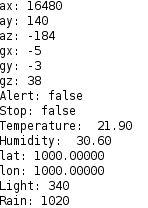
\includegraphics[width=0.3\textwidth]{datosBT.png}
\caption{Formato de un mensaje de datos que se envía a través de \textit{Bluetooth}.}
\label{fig:datosBT}
\end{center}
\end{figure}

\begin{lstlisting}[language=java,captionpos=t,caption={\textbf{Obtener datos de localización usando el dispositivo móvil.}},label={lst:location}]
LocationServices.getFusedLocationProviderClient(this).requestLocationUpdates(mLocationRequest,
  new LocationCallback() {
    @Override
    public void onLocationResult(LocationResult locationResult) {
      super.onLocationResult(locationResult);
      for (Location location : locationResult.getLocations()) {
        // Gestionar el uso de la localizacion
      }
    }
  }, null);
\end{lstlisting}

El algoritmo que comprueba si los datos recibidos tienen el formato correcto se puede ver en el Listado \ref{lst:checkFormat}. En este algoritmo se comprueba si el mensaje tiene la cantidad de datos que debería tener y si siguen la estructura de la Figura \ref{fig:datosBT}. En el caso de ser así, el mensaje se acepta y los datos del mensaje se usan en los algoritmos de análisis inteligente. En caso contrario, el mensaje se descarta.

\begin{lstlisting}[language=java,captionpos=t,caption={\textbf{Proceso de comprobación del formato de los datos recibidos por el \textit{socket Bluetooth}.}},label={lst:checkFormat}]
private boolean checkCorrectFormat(String data) {
  String header_format[] = {"ax", "ay", "az", "gx", "gy", "gz", "Alert", "Stop",
          "Temperature", "Humidity", "lat", "lon", "Light", "Rain"};

  String[] lines = data.split("\\r?\\n");

  // Check if the length of the received packet is correct
  if (lines.length == header_format.length) {
    for (int index = 0; index < lines.length; index++) {
      String[] word = lines[index].split(":");
      if (!header_format[index].equals(word[0])) {
        return false;
      }
    }
    return true;
  } else {
    return false;
  }
}
\end{lstlisting}

\subsection{Algoritmo de detección de caídas} 

\\

El algoritmo de detección de caídas usa los datos relacionados con la aceleración del usuario para, a partir de un análisis de los mismos, inferir una posible caída. Si se produce una caída, se registrará una alerta con la marca de tiempo del instante en el que se produce la caída y los datos de localización del usuario en el momento de la caída. De esta forma, el guía visualizará la alerta y podrá socorrer al participante de una forma más rápida.

El algoritmo toma como variables de entrada los valores de aceleración en los ejes $X$, $Y$, $Z$. A partir de estos valores, como se comentará a continuación, se produce un evento que produce transiciones en el estado en el que se encuentra el participante.

\begin{figure}[!h]
\begin{center}
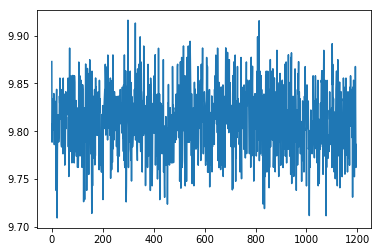
\includegraphics[width=0.6\textwidth]{parado.png}
\caption{Variación de la aceleración lineal cuando el individuo se encuentra en reposo total. La unidad de los datos de aceleración son $m/s^2$.}
\label{fig:parado}
\end{center}
\end{figure}

Si se estudia como varía la aceleración lineal de un usuario durante una caída, se pueden observar cuatro estados principales:

\begin{itemize}
\item \textbf{Estado normal}. En este estado, el usuario aún no ha sufrido la caída y se encuentra realizando una actividad diaria de forma normal. En este estado, la aceleración neta no es muy extrema ni muy distinta de la aceleración en reposo (la aceleración en reposo son $9.8$ $m/s^2$, como se puede ver en la Figura \ref{fig:parado}).
\item \textbf{Estado de caída libre}. Este estado es muy breve en el tiempo ya que comprende los instantes de tiempo desde que el usuario comienza a caer hasta que impacta con el suelo. Este estado está caracterizado por una aceleración neta muy baja, cercana a $0 m/s^2$. La aceleración de la gravedad que actúa sobre nuestro cuerpo tiene un valor de $9.8$ $m/s^2$ y mientras nuestro cuerpo está cayendo, ejerce una fuerza en sentido contrario de módulo igual (en condiciones ideales sin rozamiento) a la de la gravedad. En realidad la aceleración neta no será cero debido a que existen rozamientos, principalemente.
\item \textbf{Estado de impacto}. La transición del estado de caída libre al estado de impacto se da en el momento en el que el cuerpo del individuo impacta contra el suelo o contra cualquier otra superficie. Este estado está caracterizado por una aceleración neta muy alta. Cuando el cuerpo de un individuo colisiona contra una superficie, las fuerzas impulsivas se caracterizan por su alto módulo y su breve periodo de acción. La fuerza que ejerce una persona contra el suelo tiene el mismo módulo que la fuerza que ejerce el suelo contra la persona, pero sentido contrario. 
\item \textbf{Estado de reposo}. En este estado un individuo que ha sufrido una caída se encuentra en reposo en el suelo durante un período de tiempo variable. El estado se caracteriza por que la aceleración neta durante este período de tiempo apenas varía y está en torno a los $9.8$ $m/s^2$.
\end{itemize}

En la Figura \ref{fig:caida} se puede observar un ejemplo real de una simulación de una caída. En esta imagen se ven de forma clara los estados que se acaban de comentar y las transiciones entre ellos. De un estado de actividad normal se pasa al estado de caída libre y de este al estado de impacto para después permanecer en el estado de reposo un cierto tiempo. Cabe destacar que los estados de caída libre y de impacto son muy breves en el tiempo, como se puede ver en la imagen. Además, esta gráfica es muy similar a la que se generaría practicando una actividad cotidiana como puede ser un salto. 

\begin{figure}[!h]
\begin{center}
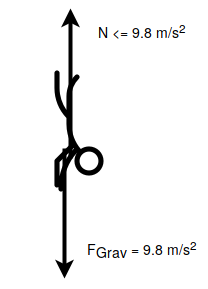
\includegraphics[width=0.3\textwidth]{fallForces.png}
\caption{Fuerzas que actúan sobre el cuerpo en caída libre (de forma ideal).}
\label{fig:fallForces}
\end{center}
\end{figure}

\begin{figure}[!h]
\begin{center}
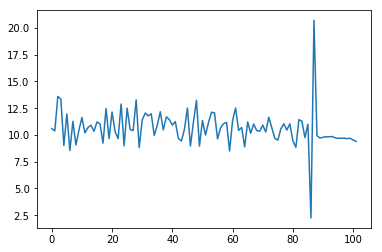
\includegraphics[width=0.6\textwidth]{caida.png}
\caption{Variación de la aceleración lineal durante una caída. La unidad de los datos de aceleración son $m/s^2$.}
\label{fig:caida}
\end{center}
\end{figure}

El algoritmo de detección de caídas que se ha implementado en este proyecto es un algoritmo de detección de caídas basado en umbrales, a partir de los datos de aceleración lineal. En este algoritmo se establecen dos umbrales, uno inferior y otro superior, que deberán ser traspasados para realizar la transición de estados. Para llevar a cabo la detección de caídas se ha diseñado una máquina de estados que tiene un total de cuatro estados:

\begin{multicols}{2}
\begin{itemize}
\item Estado normal
\item Estado de caída libre
\item Estado de impacto
\item Estado de caída
\end{itemize}
\end{multicols}

Estos estados se corresponden con los comentados anteriormente. En la Figura \ref{fig:fdDiagram} se puede ver un diagrama de estados del algoritmo de detección de caídas. El algoritmo está a la espera de recibir una serie de eventos, que son producidos por los datos de aceleración que llegan al dispositivo móvil (una descripción detallada de los eventos se puede encontrar en la Tabla \ref{table:estados}). Dependiendo del valor de los datos de aceleración se generan los eventos, utilizados para transicionar entre estados. De forma habitual, el usuario se encontrará en el estado normal. Si se supera un cierto umbral inferior, se generará un evento \texttt{LTT} y se transicionará al estado de caída libre y si, desde este estado, se supera un umbral superior se generará un evento \texttt{HTT} y se transicionará al estado de impacto. En el estado de impacto se tomarán datos durante un cierto período de tiempo y se compararán los resultados obtenidos con los que deberían obtenerse en un estado de reposo (véase Figura \ref{fig:parado}). Si ambos resultados coinciden, se generará un evento \texttt{MIT} y una caída será inferida.

\begin{table}[!h]
\centering
\begin{tabular}{|c|l|l|}
\hline
\rowcolor[HTML]{656565} 
\multicolumn{1}{|l|}{\cellcolor[HTML]{656565}{\color[HTML]{FFFFFF} Evento}} & \multicolumn{1}{c|}{\cellcolor[HTML]{656565}{\color[HTML]{FFFFFF} Descripción}}                                                                                         & \multicolumn{1}{c|}{\cellcolor[HTML]{656565}{\color[HTML]{FFFFFF} Valores que lo generan}}                                     \\ \hline
\rowcolor[HTML]{C0C0C0} 
{\color[HTML]{000000} IT}                                                   & {\color[HTML]{000000} \begin{tabular}[c]{@{}l@{}}Evento que indica que los valores \\ de aceleración se encuentran entre los \\ dos umbrales\end{tabular}}                 & {\color[HTML]{000000} \begin{tabular}[c]{@{}l@{}}Aceleración $>$ umbral inferior y\\ Aceleración $<$ umbral superior\end{tabular}} \\ \hline
\rowcolor[HTML]{C0C0C0} 
{\color[HTML]{000000} LTT}                                                  & {\color[HTML]{000000} \begin{tabular}[c]{@{}l@{}}Evento que indica que los valores \\ de aceleración están por debajo del \\ umbral inferior\end{tabular}}                 & {\color[HTML]{000000} Aceleración $\leq$ umbral inferior}                                                                      \\ \hline
\rowcolor[HTML]{C0C0C0} 
{\color[HTML]{000000} HTT}                                                  & {\color[HTML]{000000} \begin{tabular}[c]{@{}l@{}}Evento que indica que los valores \\ de aceleración están por encima del \\ umbral superior\end{tabular}}                 & {\color[HTML]{000000} Aceleración $\geq$ umbral superior}                                                                      \\ \hline
\rowcolor[HTML]{C0C0C0} 
{\color[HTML]{000000} MIT}                                                  & {\color[HTML]{000000} \begin{tabular}[c]{@{}l@{}}Evento que indica que los valores \\ durante un periodo de tiempo se \\ ajustan a la situación de reposo\end{tabular}}    & {\color[HTML]{000000} Aceleración $\approx$ $9,8$}                                                                             \\ \hline
\rowcolor[HTML]{C0C0C0} 
{\color[HTML]{000000} MNIT}                                                 & {\color[HTML]{000000} \begin{tabular}[c]{@{}l@{}}Evento que indica que los valores \\ durante un periodo de tiempo no se \\ ajustan a la situación de reposo\end{tabular}} & {\color[HTML]{000000} Aceleración distinta de $9,8$}                                                                           \\ \hline
\end{tabular}
\caption{Descripción de los los eventos que se pueden generar en el algoritmo de detección de caídas y los valores de aceleración que los generan.}
\label{table:estados}
\end{table}

\begin{figure}[!h]
\begin{center}
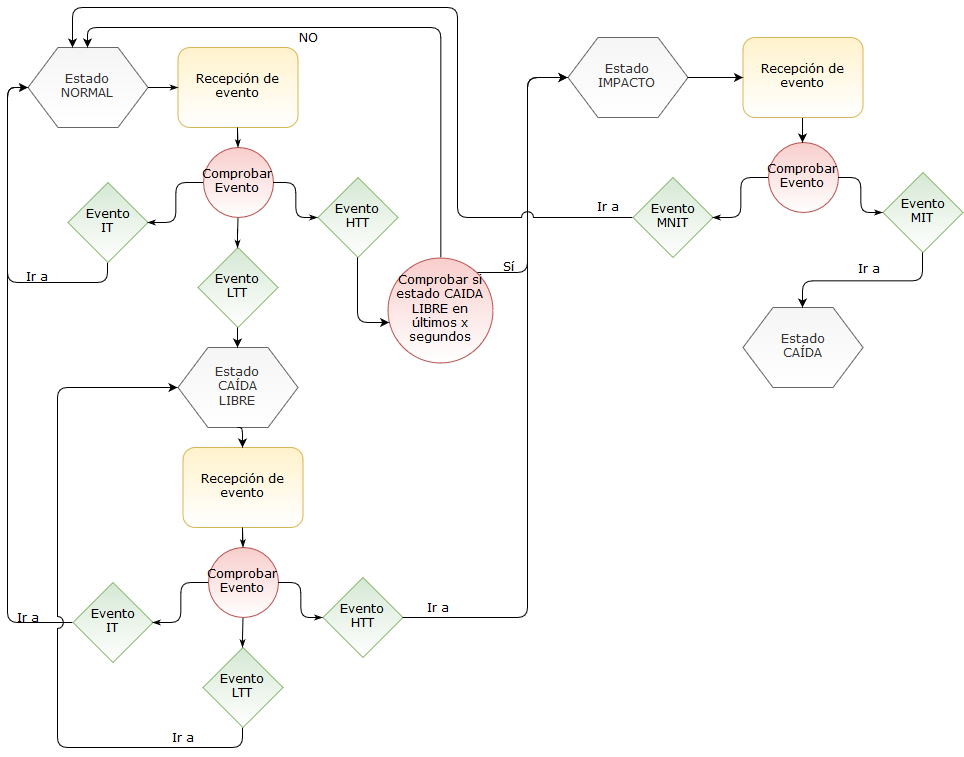
\includegraphics[width=\textwidth]{FD_ExtendedDiagram.png}
\caption{Diagrama de estados del algoritmo de detección de caídas.}
\label{fig:fdDiagram}
\end{center}
\end{figure}

Una consideración importante que se ha tenido en cuenta en el algoritmo de detección de caídas es el posible ruido existente en los datos. Es posible que se esté recibiendo información de caída libre y justo después se reciba un evento de datos dentro de los dos umbrales que haría al algoritmo transicionar al estado de normalidad (esto se puede dar simplemente por ruido en los datos o incluso porque un hilo que gestiona datos anteriores de normalidad se ejecute más lentamente que un hilo creado posteriormente con datos de caída libre). Se contempla que si en los siguientes instantes se recibe un evento de superación del umbral superior, la información relativa al estado de normalidad es ruido y se transiciona de forma directa al estado de impacto.

\begin{lstlisting}[language=java,captionpos=t,caption={\textbf{Creación de eventos a partir de los datos de aceleración y transición a otro estado.}},label={lst:eventFD}]
FD_Event event_occurred;
if (force < 0.65 * G) {
  event_occurred = FD_Event.FD_DataLessThreshold;
} else if (force > 2.5 * G) {
  event_occurred = FD_Event.FD_DataMoreThreshold;
} else {
  event_occurred = FD_Event.FD_DataInsideThreshold;
}

FallDetector fallDetector = FallDetector.getInstance();
fallDetector.makeTransition(event_occurred, force);
\end{lstlisting}

En el Listado \ref{lst:eventFD} se puede observar el código asociado a la creación de un cierto evento a partir de los datos de aceleración. El valor de aceleración que se compara con los umbrales es el resultado de aplicar la fórmula:

\begin{equation}
\begin{center}
$|\vec{a}| = \sqrt{a_x^2 + a_y^2 + a_z^2}$
\end{center}
\end{equation}

Los valores de aceleración que se han establecido como umbrales son $2.5g$ (o $24.5$ $m/s^2$) para el umbral superior y $0.65g$ o ($\approx 6.4$ $m/s^2$) para el umbral inferior. Los valores se han establecido tanto empíricamente (a base de distintas pruebas de caídas simuladas) y gracias a otros trabajos en algoritmos de detección de caídas basados en umbrales como pueden ser los encontrados en \cite{44}, \cite{45} y \cite{46}.

El algoritmo que implementa el diagrama de la Figura \ref{fig:fdDiagram}, está basado en una máquina de estados. La máquina de estados sigue un patrón de diseño \textit{singleton}, de forma que sólo hay una instancia de la máquina de estados en todo el código. Como todos los hilos gestionan la misma instancia de la máquina de estados (no tiene sentido tener varios objetos, pues el estado en el que el usuario se encuentra es único y global), la transición entre estados se debe hacer en términos de exclusión mutua. Se puede observar en el Listado \ref{lst:mutex}} como el hilo que se dispone a hacer una transición de estados tiene que tomar el control del semáforo \texttt{mutex} que gobierna la sincronización en los accesos.

\begin{lstlisting}[language=java,captionpos=t,caption={\textbf{Exclusión mutua en la transición entre estados, en el algoritmo de detección de caídas.}},label={lst:mutex}]
public void makeTransition(FD_Event event, double data) {
  try {
    mutex.acquire(1);
    // Logica de la transicion
  } catch (Exception ex) {
    // Control de errores
  } finally {
    mutex.release(1);
  }
}
\end{lstlisting}

Como se puede ver en el Listado \ref{lst:StateMachine}, la matriz de transiciones almacena todas las posibles transiciones de la maquina de estados. Cada entrada tiene el siguiente formato:

\begin{center}
$($Estado en el que se está, Evento que se produce$)$, Estado al que se transiciona
\end{center}

\begin{lstlisting}[language=java,captionpos=t,caption={\textbf{Máquina de estados que gestiona las transiciones entre estados, a partir de eventos generados.}},label={lst:StateMachine}]
transition_matrix.put(Pair.create(FD_State.FD_NORMAL, FD_Event.FD_DataInsideThreshold), FD_State.FD_NORMAL);
transition_matrix.put(Pair.create(FD_State.FD_NORMAL, FD_Event.FD_DataMoreThreshold), FD_State.FD_NORMAL);
transition_matrix.put(Pair.create(FD_State.FD_NORMAL, FD_Event.FD_DataLessThreshold), FD_State.FD_FREE_FALL);

transition_matrix.put(Pair.create(FD_State.FD_FREE_FALL, FD_Event.FD_DataInsideThreshold), FD_State.FD_NORMAL);
transition_matrix.put(Pair.create(FD_State.FD_FREE_FALL, FD_Event.FD_DataLessThreshold), FD_State.FD_FREE_FALL);
transition_matrix.put(Pair.create(FD_State.FD_FREE_FALL, FD_Event.FD_DataMoreThreshold), FD_State.FD_IMPACT);

...
\end{lstlisting}

\subsection{Grado de dispersión del grupo}

El grado de dispersión del grupo es un posible indicador de riesgo en la expedición. Un alto grado de dispersión significa que el grupo de expedición está muy separado, por lo que una posible alerta de un participante demasiado lejos puede tardar más en ser atendida, con los riesgos que esto conlleva. El guía puede usar este valor para decidir realizar una parada de reagrupación, o al menos reducir el ritmo de marcha hasta que todos los usuarios están agrupados. Un alto grado de dispersión en el grupo puede indicar también síntomas de fatiga en los participantes que se encuentran mas rezagados. Esta fatiga puede acarrear otros problemas como la deshidratación o posibles caídas, por lo que es recomendable tenerla controlada.

El grado de dispersión del grupo se mide como la media de las distancias entre el guía y los participantes:

\begin{itemize}
\item Sea $g$ el guía de la expedición.
\item Sea $\mathcal{P}$ el conjunto de todos los participantes de la expedición.
\item Sea $n$ el tamaño del conjunto $\mathcal{P}$.
\item Sea $distancia(a, b)$ la distancia de \textit{Harvesine}\footnote{La distancia de \textit{Harvesine} se explica más a fondo en la Sección \ref{MapaRecorrido}} existente entre dos usuarios $a$ y $b$, con coordenadas $(Lat_a, Lon_a)$ y $(Lat_b, Lon_b)$ en una circunferencia de radio $r$:\\
\begin{center}
\begin{equation}
distancia(a,b) = 2\cdot r \cdot $ \\ $\arcsin{\left( \sqrt{\sin^2\left(\frac{Lat_b - Lat_a}{2} \right) + \cos \left( Lat_a \right) \cdot \cos \left( Lat_b \right) \cdot \sin^2 \left( \frac{Lon_b - Lon_a}{2} \right)}\right)}
\end{equation}
\end{center}
\end{itemize}

Entonces:

\begin{center}
\begin{equation}
$Grado de dispersión$ = \frac{1}{n} \cdot \sum_{i=1}^{n}distancia(g, p), \forall p \in \mathcal{P}
\end{equation}
\end{center}

Póngase como ejemplo un grupo de expedición en el que participan cuatro usuarios (tres de ellos actúan como participantes y uno como guía). Se suponen las siguientes distancias de separación (calculadas usando la fórmula de \textit{Harvesine}) entre el guía y los participantes:

\begin{itemize}
\item Distancia entre guía y participante 1 $= 0.3km$
\item Distancia entre guía y participante 2 $= 0.1km$
\item Distancia entre guía y participante 3 $= 0.8km$
\end{itemize}

El grado de dispersión del grupo será $\frac{1}{3} \cdot (0.3 + 0.1 + 0.8) = \frac{1}{3} \cdot 1.2 = 0.4km$

\subsection{Análisis del riesgo de caída en la expedición de cada integrante de la misma}
\label{analysis_risk}

Realizar un análisis del riesgo de caída existente en un cierto instante de tiempo resulta una gran ayuda tanto para los participantes como para el guía. Gracias a este análisis, los participantes pueden visualizar el riesgo al que están expuestos en un determinado momento por lo que pueden poner los medios de su parte para intentar minimizar ese riesgo por ejemplo, aminorando la velocidad, haciendo uso de una linterna si las condiciones de luz son desfavorables o poniéndose al resguardo de la lluvia en el caso de haber una tormenta. Del mismo modo, el riesgo de caída es también muy útil para el guía, que en función de éste puede decidir realizar una parada para la reagrupación total del grupo, y así tener controlados a todos los participantes del mismo. El riesgo de caída de un integrante en la expedición depende de varios factores, como por ejemplo la cantidad de luz que existe en el entorno en el que se encuentran, la humedad que podría dificultar la estabilidad del terreno y las condiciones climatológicas adversas, como la lluvia, que hacen que el terreno por el que se mueven los usuarios presente un mayor riesgo de caída. Todos ellos, debidamente combinados, nos pueden reportar información realmente útil para determinar el riesgo de caída durante la expedición.

Para realizar el análisis del riesgo de caída en el presente proyecto, se ha decidido hacer uso de la \textbf{lógica difusa}. La lógica difusa \cite{43} proporciona un mecanismo de inferencia que permite simular los procedimientos de razonamiento humano en sistemas basados en el conocimiento. El cálculo del riesgo de caída es un problema en el que existe incertidumbre y vaguedad en los datos ya que no es posible afirmar con certeza si un usuario en una ruta de expedición va a sufrir una caída o no. Por lo tanto, este modelo matemático es el apropiado para lidiar con esta problemática.

La lógica difusa se trata de un modelo matemático adecuado para tratar la incertidumbre y la vaguedad de los datos, dos situaciones que se plantean en este proyecto. Existe incertidumbre ya que no se puede asegurar con precisión si un usuario se caerá en una cierta situación. Existe vaguedad en los datos (sobre todo con los datos de humedad y luz) ya que no se puede precisar si un cierto valor de humedad o luz pertenece a un conjunto (por ejemplo, no tiene sentido inferir que una humedad del 74\% es una humedad media y una humedad del 75\% es una humedad alta).

\begin{table}[!h]
\centering
\begin{tabular}{|c|c|c|c|}
\hline
\rowcolor[HTML]{656565} 
{\color[HTML]{FFFFFF} \textbf{\begin{tabular}[c]{@{}c@{}}Variable\\ de Entrada\end{tabular}}} & {\color[HTML]{FFFFFF} \textbf{\begin{tabular}[c]{@{}c@{}}Dominio\\ de Definición\end{tabular}}} & {\color[HTML]{FFFFFF} \textbf{\begin{tabular}[c]{@{}c@{}}Conjunto\\ Difuso\end{tabular}}} & {\color[HTML]{FFFFFF} \textbf{\begin{tabular}[c]{@{}c@{}}Rango de\\ Valores\end{tabular}}} \\ \hline
\rowcolor[HTML]{EFEFEF} 
\cellcolor[HTML]{EFEFEF}{\color[HTML]{000000} }                                               & \cellcolor[HTML]{EFEFEF}{\color[HTML]{000000} }                                                 & {\color[HTML]{000000} Sí}                                                                 & {\color[HTML]{000000} {[}0 - 562{]}}                                                       \\ \cline{3-4} 
\rowcolor[HTML]{EFEFEF} 
\multirow{}{}{\cellcolor[HTML]{EFEFEF}{\color[HTML]{000000} Lluvia}}                       & \multirow{}{}{\cellcolor[HTML]{EFEFEF}{\color[HTML]{000000} {[}0 - 1023{]}}}                 & {\color[HTML]{000000} No}                                                                 & {\color[HTML]{000000} {[}462 - 1023{]}}                                                    \\ \hline
\rowcolor[HTML]{FFFFFF} 
\cellcolor[HTML]{FFFFFF}{\color[HTML]{000000} }                                               & \cellcolor[HTML]{FFFFFF}{\color[HTML]{000000} }                                                 & {\color[HTML]{000000} Muy Oscuro}                                                           & {\color[HTML]{000000} {[}0 - 200{]}}                                                       \\ \cline{3-4} 
\rowcolor[HTML]{FFFFFF} 
\cellcolor[HTML]{FFFFFF}{\color[HTML]{000000} }                                               & \cellcolor[HTML]{FFFFFF}{\color[HTML]{000000} }                                                 & {\color[HTML]{000000} Oscuro}                                                             & {\color[HTML]{000000} {[}100 - 400{]}}                                                     \\ \cline{3-4} 
\rowcolor[HTML]{FFFFFF} 
\cellcolor[HTML]{FFFFFF}{\color[HTML]{000000} }                                               & \cellcolor[HTML]{FFFFFF}{\color[HTML]{000000} }                                                 & {\color[HTML]{000000} Media}                                                              & {\color[HTML]{000000} {[}300 - 600{]}}                                                     \\ \cline{3-4} 
\rowcolor[HTML]{FFFFFF} 
\cellcolor[HTML]{FFFFFF}{\color[HTML]{000000} }                                               & \cellcolor[HTML]{FFFFFF}{\color[HTML]{000000} }                                                 & {\color[HTML]{000000} Media-alta}                                                             & {\color[HTML]{000000} {[}500 - 900{]}}                                                     \\ \cline{3-4} 
\rowcolor[HTML]{FFFFFF} 
\multirow{}{}{\cellcolor[HTML]{FFFFFF}{\color[HTML]{000000} Luz}}                          & \multirow{}{}{\cellcolor[HTML]{FFFFFF}{\color[HTML]{000000} {[}0 - 1023{]}}}                 & {\color[HTML]{000000} Máxima}                                                          & {\color[HTML]{000000} {[}800 - 1023{]}}                                                    \\ \hline
\rowcolor[HTML]{EFEFEF} 
\cellcolor[HTML]{EFEFEF}{\color[HTML]{000000} }                                               & \cellcolor[HTML]{EFEFEF}{\color[HTML]{000000} }                                                 & {\color[HTML]{000000} Muy baja}                                                           & {\color[HTML]{000000} {[}0 -20{]}}                                                         \\ \cline{3-4} 
\rowcolor[HTML]{EFEFEF} 
\cellcolor[HTML]{EFEFEF}{\color[HTML]{000000} }                                               & \cellcolor[HTML]{EFEFEF}{\color[HTML]{000000} }                                                 & {\color[HTML]{000000} Baja}                                                               & {\color[HTML]{000000} {[}10 - 40{]}}                                                       \\ \cline{3-4} 
\rowcolor[HTML]{EFEFEF} 
\cellcolor[HTML]{EFEFEF}{\color[HTML]{000000} }                                               & \cellcolor[HTML]{EFEFEF}{\color[HTML]{000000} }                                                 & {\color[HTML]{000000} Media}                                                              & {\color[HTML]{000000} {[}30 - 60{]}}                                                       \\ \cline{3-4} 
\rowcolor[HTML]{EFEFEF} 
\cellcolor[HTML]{EFEFEF}{\color[HTML]{000000} }                                               & \cellcolor[HTML]{EFEFEF}{\color[HTML]{000000} }                                                 & {\color[HTML]{000000} Alta}                                                               & {\color[HTML]{000000} {[}50 - 80{]}}                                                       \\ \cline{3-4} 
\rowcolor[HTML]{EFEFEF} 
\multirow{}{}{\cellcolor[HTML]{EFEFEF}{\color[HTML]{000000} Humedad}}                      & \multirow{}{}{\cellcolor[HTML]{EFEFEF}{\color[HTML]{000000} {[}0 -100{]}}}                   & {\color[HTML]{000000} Muy alta}                                                           & {\color[HTML]{000000} {[}70 - 100{]}}                                                      \\ \hline
\end{tabular}
\caption{Variables de entrada y conjuntos difusos de dichas variables, del algoritmo de riesgo de caída.}
\label{table:inputVariablesAndSets}
\end{table}

\begin{table}[!h]
\centering
\begin{tabular}{|c|c|c|c|}
\hline
\rowcolor[HTML]{656565} 
{\color[HTML]{FFFFFF} \textbf{\begin{tabular}[c]{@{}c@{}}Variable\\ de Salida\end{tabular}}} & {\color[HTML]{FFFFFF} \textbf{\begin{tabular}[c]{@{}c@{}}Dominio\\ de definición\end{tabular}}} & {\color[HTML]{FFFFFF} \textbf{\begin{tabular}[c]{@{}c@{}}Conjunto\\ Difuso\end{tabular}}} & {\color[HTML]{FFFFFF} \textbf{\begin{tabular}[c]{@{}c@{}}Rango de\\ Valores\end{tabular}}} \\ \hline
\rowcolor[HTML]{EFEFEF} 
\cellcolor[HTML]{EFEFEF}{\color[HTML]{000000} }                                              & \cellcolor[HTML]{EFEFEF}{\color[HTML]{000000} }                                                 & {\color[HTML]{000000} Bajo}                                                               & {\color[HTML]{000000} {[}0 - 0.4{]}}                                                       \\ \cline{3-4} 
\rowcolor[HTML]{EFEFEF} 
\cellcolor[HTML]{EFEFEF}{\color[HTML]{000000} }                                              & \cellcolor[HTML]{EFEFEF}{\color[HTML]{000000} }                                                 & {\color[HTML]{000000} Medio}                                                              & {\color[HTML]{000000} {[}0.3 - 0.8{]}}                                                     \\ \cline{3-4} 
\rowcolor[HTML]{EFEFEF} 
\multirow{}{}{\cellcolor[HTML]{EFEFEF}{\color[HTML]{000000} Riesgo}}                      & \multirow{}{}{\cellcolor[HTML]{EFEFEF}{\color[HTML]{000000} {[}0 - 1{]}}}                    & {\color[HTML]{000000} Alto}                                                               & {\color[HTML]{000000} {[}0.7 - 1{]}}                                                       \\ \hline
\end{tabular}
\caption{Variable de salida y conjuntos difusos de dicha variable, del algoritmo de riesgo de caída.}
\label{table:outputVariablesAndSets}
\end{table}

Los conjuntos difusos permiten a sus elementos tener un grado de pertenencia a los mismos. La lógica difusa emplea valores continuos entre 0 (pertenencia nula a un conjunto difuso) y 1 (pertenencia total a un conjunto difuso). Mediante el proceso de \textit{fuzzificación}, los valores de las distintas variables de entrada se asocian con los conjuntos difusos definidos (véase Tabla \ref{table:inputVariablesAndSets}). Una vez se ha realizado la \textit{fuzzificación}, se aplican reglas lingüísticas para obtener una salida (véase Tabla \ref{table:outputVariablesAndSets}). Esta salida se puede \textit{defuzzificar} (para obtener un valor discreto) o tratarse de forma \textit{fuzzificada} (en lenguaje natural). En este proyecto, la salida se trata de forma \textit{fuzzificada}, ya que los usuarios de la expedición sólo necesitan saber el riesgo de caída mediante una etiqueta lingüística (alto, medio o bajo), sin necesidad de conocer un valor numérico preciso.

La función de pertenencia, asociada a cada variable, define el grado de pertenencia de un cierto valor de entrada a un conjunto difuso. El valor de entrada se puede \textit{fuzzificar} asignando la etiqueta lingüística asociada a un conjunto difuso. Una vez que se tienen \textit{fuzzificados} los valores de todas las variables de entrada, comienza el proceso de inferencia haciendo uso del conjunto de reglas definidas, que siguen el formato:

\textit{Si variable de entrada pertenece a un conjunto $x$ $\rightarrow$ variable de salida pertenece al conjunto $y$}

Cabe destacar que la sentencia condicional anterior se puede extender mediante el uso de operadores lógicos (\textit{and}, \textit{or} y \textit{not} lógicos) para encadenar varias condiciones en una misma regla. Las reglas que se han diseñado en este proyecto se pueden observar a continuación: 

\begin{itemize}
\item \textbf{R1.} Si lluvia es sí $\wedge$ (luz es media-alta $\vee$ luz es máxima) $\wedge$ (humedad es muy baja $\vee$ humedad es baja $\vee$ humedad es media) $\rightarrow$ riesgo es bajo
\item \textbf{R2.} Si lluvia es sí $\wedge$ (luz es media-alta $\vee$ luz es máxima) $\wedge$ (humedad es alta $\vee$ humedad muy alta) $\rightarrow$ riesgo es medio
\item \textbf{R3.} Si lluvia es sí $\wedge$ luz es media $\wedge$ (humedad es muy baja $\vee$ humedad es baja $\vee$ humedad es media) $\rightarrow$ riesgo es medio
\item \textbf{R4.} Si lluvia es sí $\wedge$ (luz es oscuro $\vee$ luz es muy oscuro) $\rightarrow$ riesgo es alto
\item \textbf{R5.} Si lluvia es sí $\wedge$ luz es media $\wedge$ (humedad es alta $\vee$ humedad muy alta) $\rightarrow$ riesgo es alto
\item \textbf{R6.} Si lluvia es no $\wedge$ (luz es media-alta $\vee$ luz es máxima) $\rightarrow$ riesgo es bajo
\item \textbf{R7.} Si lluvia es no $\wedge$ luz es media $\wedge$ (humedad es muy baja $\vee$ humedad es baja $\vee$ humedad es media) $\rightarrow$ riesgo es bajo
\item \textbf{R8.} Si lluvia es no $\wedge$ luz es media $\wedge$ (humedad es alta $\vee$ humedad muy alta) $\rightarrow$ riesgo es medio
\item \textbf{R9.} Si lluvia es no $\wedge$ luz es oscuro $\wedge$ (humedad es muy baja $\vee$ humedad es baja $\vee$ humedad es media) $\rightarrow$ riesgo es medio
\item \textbf{R10.} Si lluvia es no $\wedge$ luz es oscuro $\wedge$ (humedad es alta $\vee$ humedad muy alta) $\rightarrow$ riesgo es alto
\item \textbf{R11.} Si lluvia es no $\wedge$ luz es muy oscuro $\wedge$ (humedad es muy baja $\vee$ humedad es baja) $\rightarrow$ riesgo es medio
\item \textbf{R12.} Si lluvia es no $\wedge$ luz es muy oscuro $\wedge$ (humedad es media $\vee$ humedad es alta $\vee$ humedad muy alta) $\rightarrow$ riesgo es alto
\end{itemize}

En el Listado \ref{lst:fuzzyRules} se puede observar la correspondencia de alguna de las anteriores reglas en código \texttt{Java}.

Para implementar la lógica difusa en la aplicación \textit{Android}, se ha usado la librería \texttt{jfuzzylogic}\footnote{\url{http://jfuzzylogic.sourceforge.net/html/index.html}}. Esta librería usa varios tipos de \textit{defuzzificadores}, de reglas de agregación, de reglas de implicación y de operadores de conexión entre reglas, de forma que se adapta a la situación en la que se vaya a usar de forma muy fácil. 

En este proyecto se usa el máximo como regla de agregación y el \textit{defuzzificador} \textit{centroid}.

En las Figuras \ref{fig:fuzzyHumiAndRain} y \ref{fig:fuzzyLightaAndRisk} se pueden observar entre qué valores (del dominio de definición de la variable) se encuentran los distintos conjuntos difusos.

\begin{figure}[!h]
\begin{center}
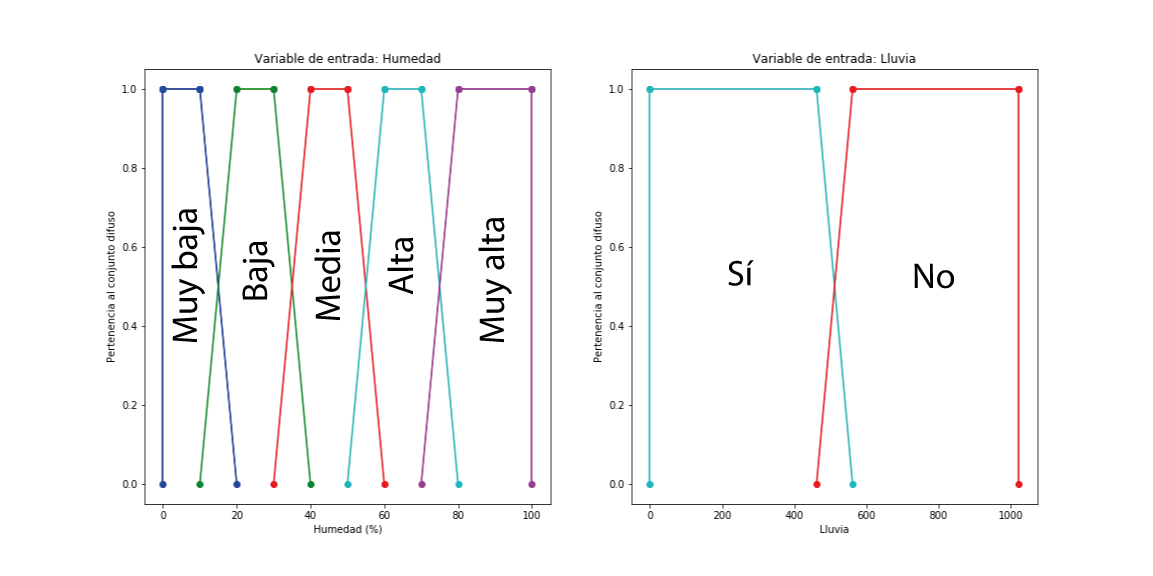
\includegraphics[width=\textwidth]{fuzzyHumiAndRain.png}
\caption{Valores de los conjuntos difusos, de las variables de entrada de humedad y lluvia.}
\label{fig:fuzzyHumiAndRain}
\end{center}
\end{figure}

\begin{figure}[!h]
\begin{center}
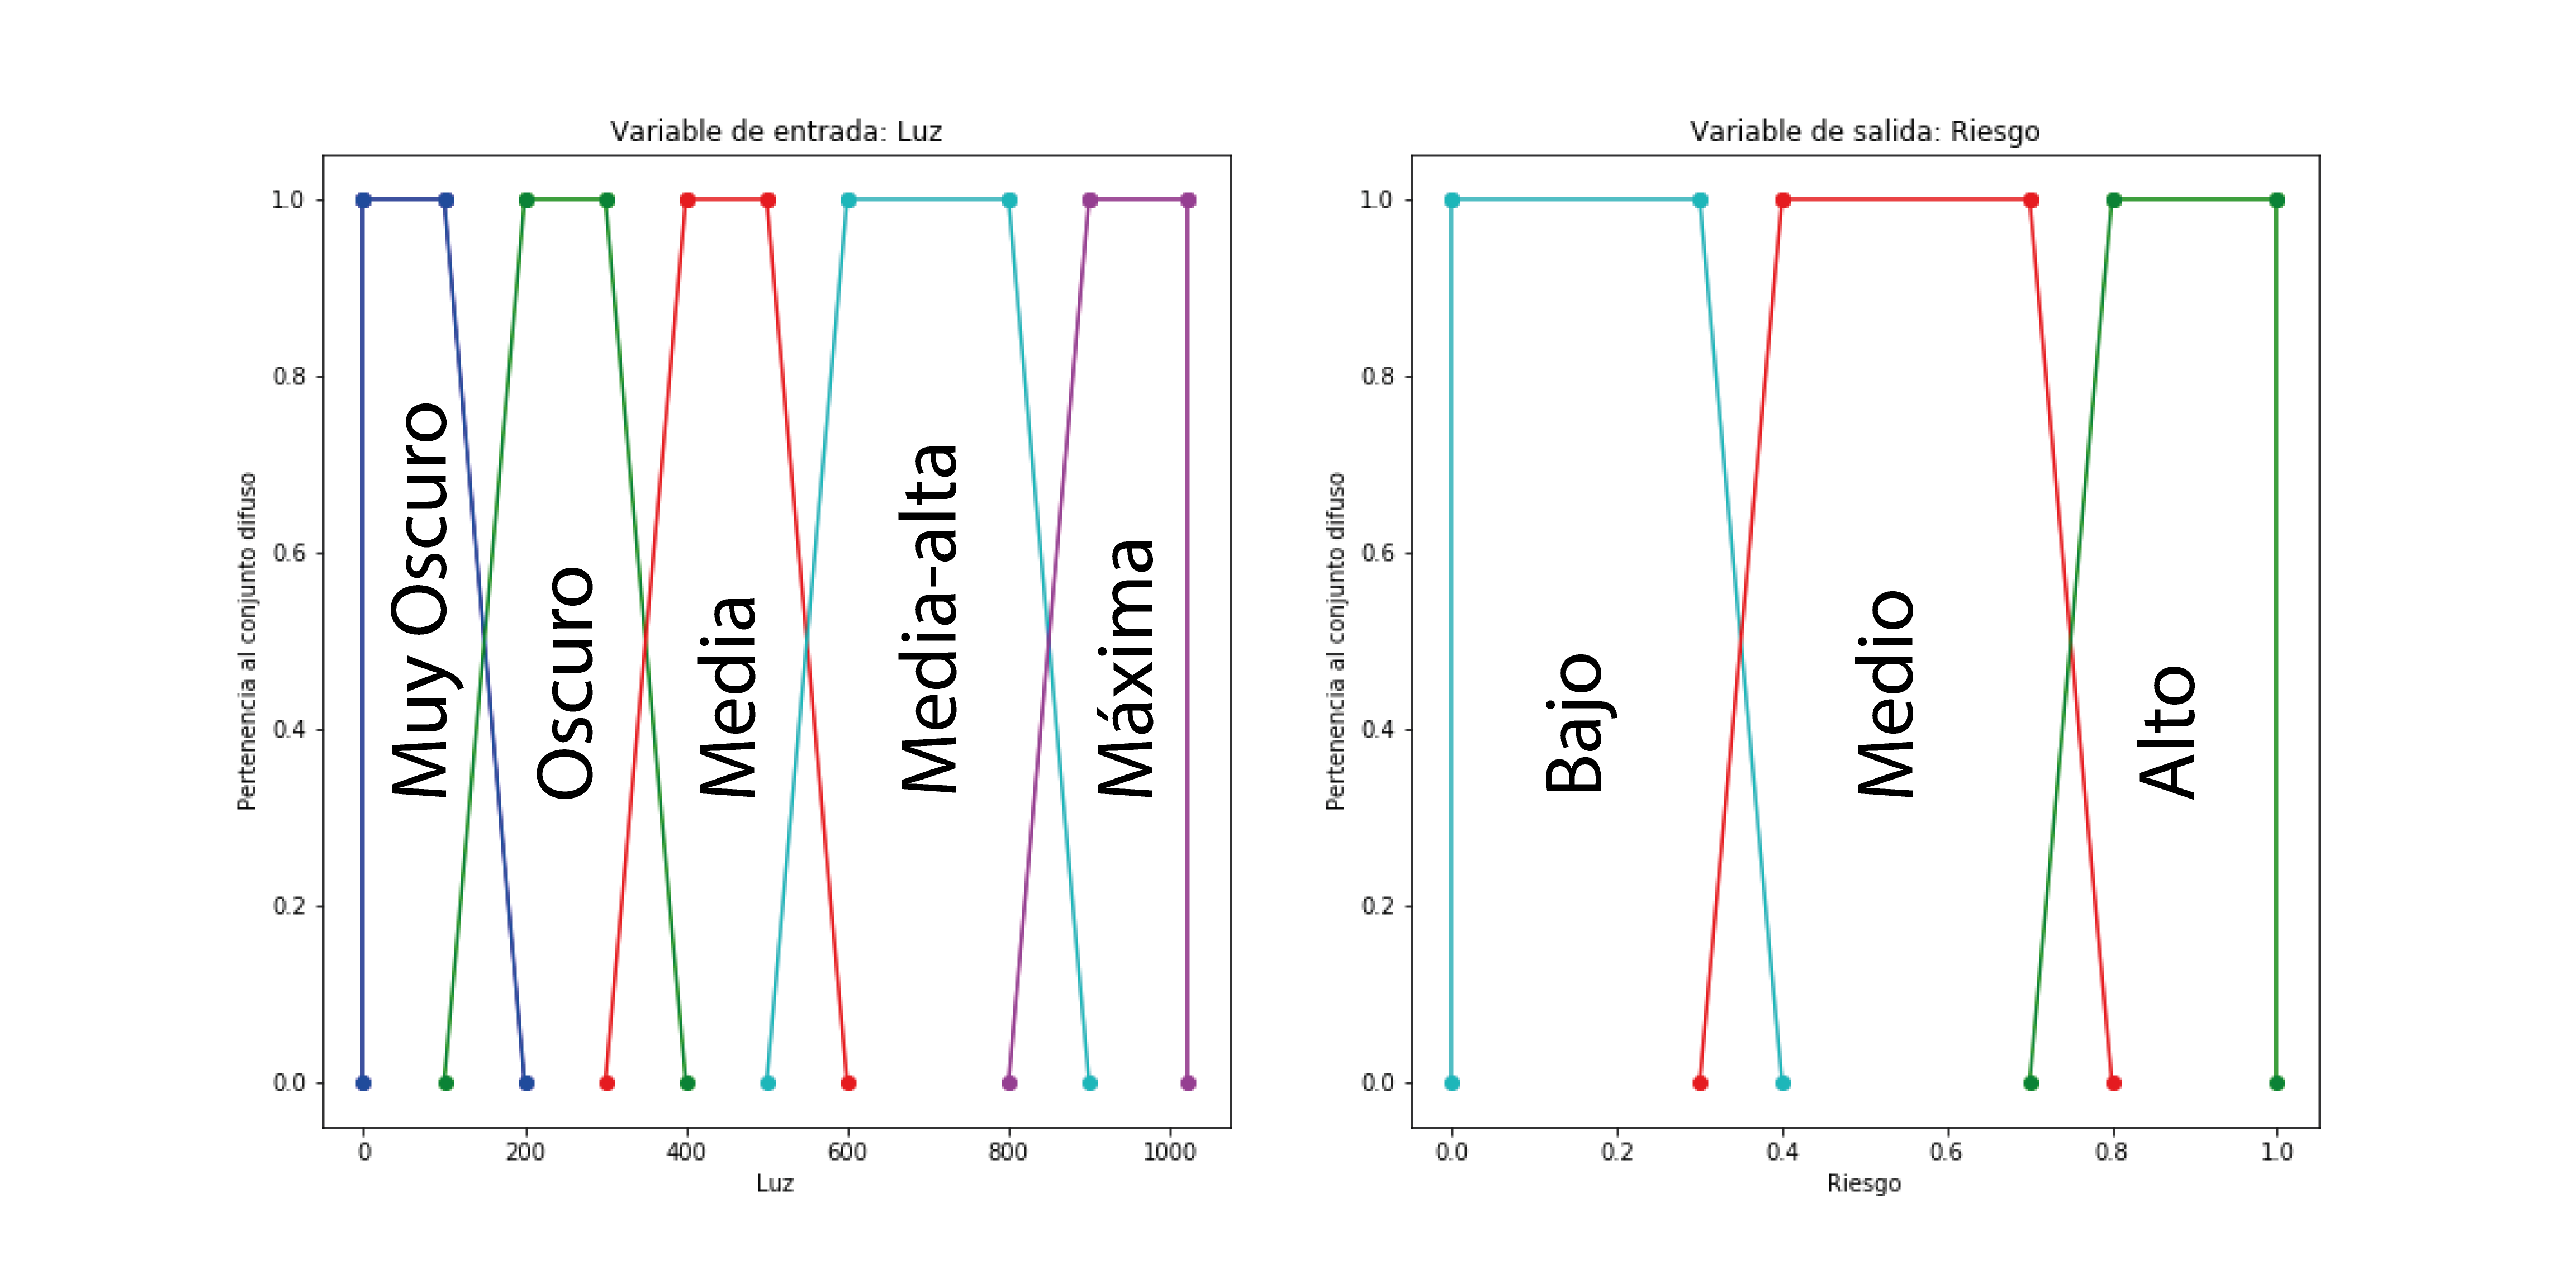
\includegraphics[width=\textwidth]{fuzzyLightaAndRisk.png}
\caption{Valores de los conjuntos difusos, de la variable de entrada de luz y la variable de salida de riesgo.}
\label{fig:fuzzyLightaAndRisk}
\end{center}
\end{figure}

\begin{lstlisting}[language=java,captionpos=t,caption={\textbf{Algunas de las reglas difusas definidas para obtener el grado de pertenencia de una variable de salida a los conjuntos difusos.}},label={lst:fuzzyRules}]
ruleBlock.addRule(Rule.parse("if rain is yes and (light is midhigh or light is maximum) and (humidity is veryLow or humidity is low or humidity is mid) then risk is low", engine));
ruleBlock.addRule(Rule.parse("if rain is yes and (light is midhigh or light is maximum) and (humidity is high or humidity is veryHigh) then risk is mid", engine));
ruleBlock.addRule(Rule.parse("if rain is yes and light is mid and (humidity is veryLow or humidity is low or humidity is mid) then risk is mid", engine));
ruleBlock.addRule(Rule.parse("if (humidity is high or humidity is veryHigh) and rain is yes then risk is high", engine));
...
\end{lstlisting}

Entre las ventajas del uso de la lógica difusa en este proyecto destacan:

\begin{itemize}
\item Mayor interpretabilidad de los datos de salida para los usuarios, ya que visualizan etiquetas lingüísticas que son más familiares que un valor numérico de riesgo de caída.
\item Una regla difusa equivale a múltiples reglas normales, por lo que puede cubrir una gran cantidad de casos.
\item Si en algún momento se quiere cambiar el comportamiento del algoritmo, solo es necesario redefinir las reglas (añadiendo nuevas reglas o modificando o eliminando las reglas existentes) o variar los dominios de definición de las variables de entrada y salida.
\item La inclusión de nuevos sensores que formen parte del análisis del riesgo de caída es sencilla. Tan sólo es necesario crear una nueva variable de entrada y añadir nuevas reglas que la incluyan.
\end{itemize}

\section{Plataforma \textit{web}}
\label{platformweb}

En esta sección se muestra el diseño y la implementación de la plataforma \textit{web}, encargada de la visualización (tanto en tiempo real como de forma histórica) de la información relacionada con las expediciones. La plataforma \textit{web} sigue una arquitectura cliente-servidor, en la que el \textit{backend} se ha desarrollado usando \texttt{node-js} y el \textit{frontend} ha sido desarrollado usando \texttt{react}.

\subsection{Diseño de la plataforma \textit{web}}

Como se ha comentado anteriormente, el \textit{frontend} de la plataforma \textit{web} se ha desarrollado usando \texttt{React}, una librería basada en componentes y escrita en \texttt{Javascript}. \texttt{React} es una librería que se utiliza para crear la interfaz de usuario de la página \textit{web} a través de componentes. Un componente es un elemento visual que forma parte de la interfaz, que tiene su propio estado e implementa su propia lógica de renderizado, por lo que una misma vista se puede componer por varios componentes que se podrán mostrar en pantalla de formas distintas, de acuerdo a la lógica de renderizado de cada uno de los componentes. Para desarrollar el \textit{frontend}, además de \texttt{React} se ha usado \texttt{Bootstrap} con el objetivo de realizar un diseño \textit{responsive} que se adapte a distintos tamaños de pantalla (ordenador, móvil o \textit{tablet} entre otros). 

La arquitectura del sistema \textit{web} se puede observar en la Figura \ref{fig:webarch}. El usuario interacciona con el sistema a través de la interfaz de usuario que éste proporciona. Dependiendo de la acción, se generarán peticiones \ac{HTTP} (\texttt{GET} y \texttt{POST}) a una \ac{API} de funciones expuestas en el servidor \texttt{Express}. Estas funciones se encargarán de las tareas de gestión de usuarios (autenticación y deautenticación de los mismos) y gestión de las expediciones (obtener las expediciones de un usuario, obtener información detallada acerca de una expedición en concreto, obtener las alertas de un participante, etc.). Una vez que la información que ha sido solicitada por el \textit{frontend} a través de la petición \ac{HTTP} está lista, el \textit{backend} responde a la petición con dicha información.

\begin{figure}[!h]
\begin{center}
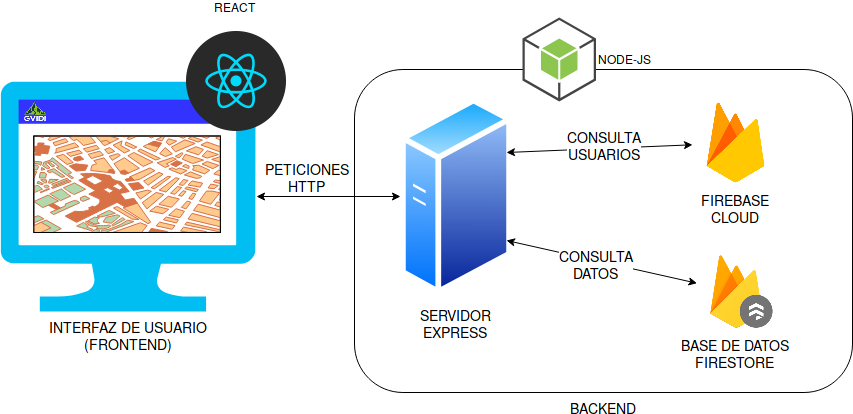
\includegraphics[width=\textwidth]{web_architecture.png}
\caption{Arquitectura de la plataforma \textit{web}.}
\label{fig:webarch}
\end{center}
\end{figure}

En las Figuras \ref{fig:signinWeb} a \ref{fig:mapainfo} se puede observar la interfaz de usuario de la plataforma \textit{web}. Cabe destacar la visualización sobre el mapa en tiempo real de la expedición. Sobre este mapa también se mostrarán las alertas (de caídas, pérdida de miembro del grupo o excesiva distancia con respecto al guía) si las hubiera. Si se hace \textit{click} sobre alguna de las alertas o sobre cualquier otro punto en la ruta sobre el mapa, debajo del mismo se mostrará una tarjeta con información detallada de la expedición en ese punto. 

\begin{figure}
\centering
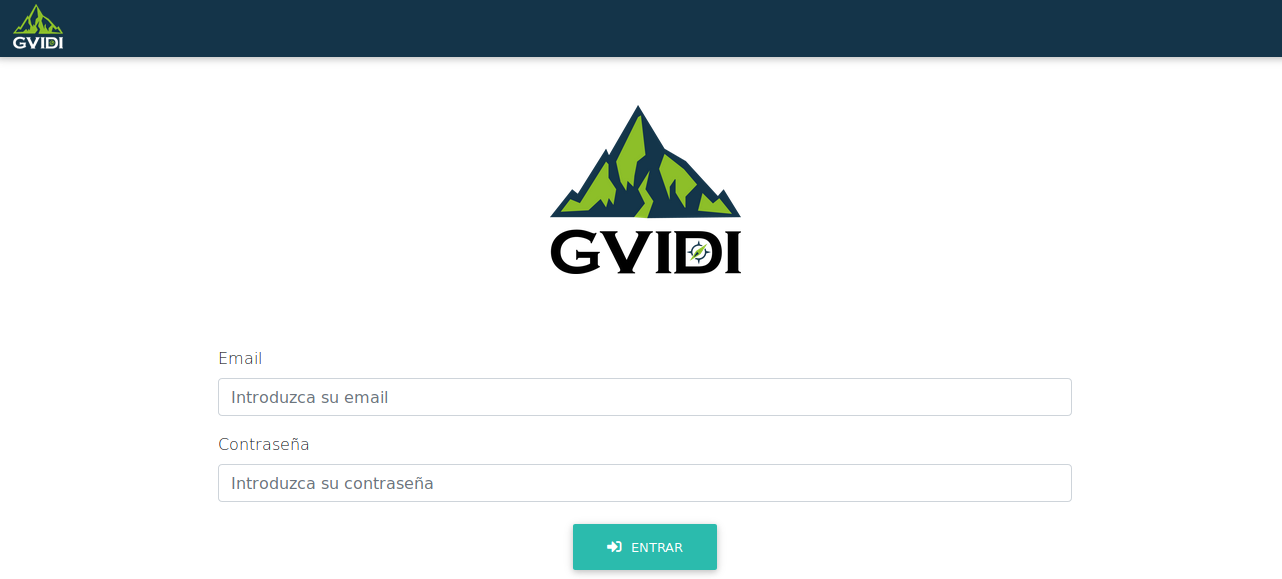
\includegraphics[width=0.8\textwidth]{login_web.png}
\caption{Página de \textit{Login} de la \textit{web}.}
\label{fig:signinWeb}
\end{figure}
 
\begin{figure} 
\centering
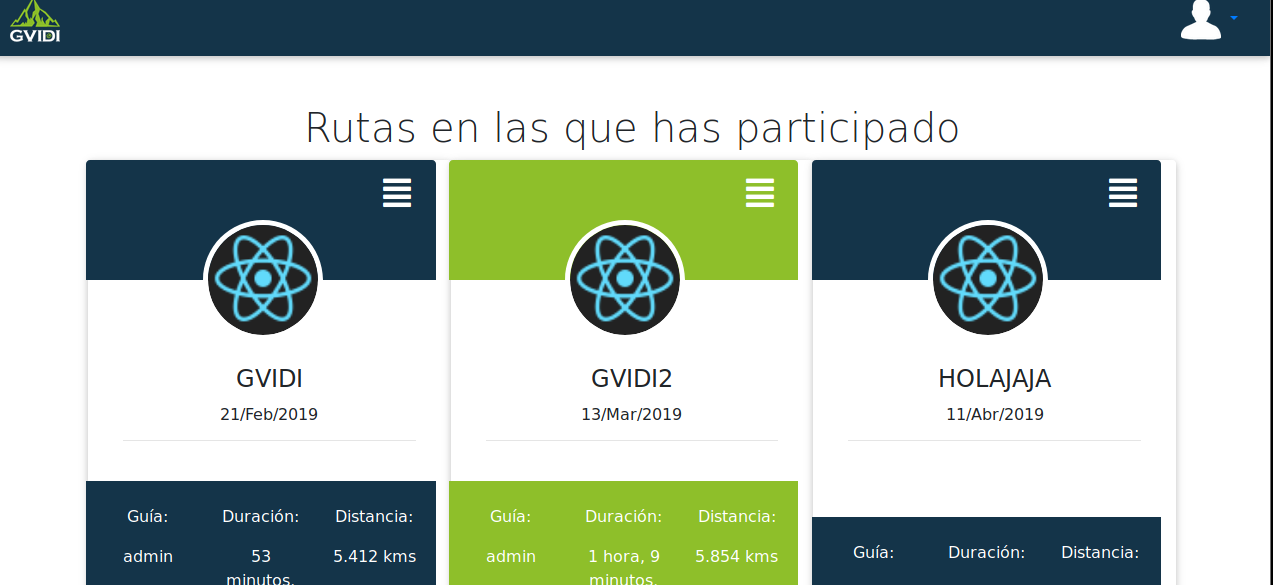
\includegraphics[width=0.8\textwidth]{todasRutas.png}}
\caption{Página que contiene el histórico de rutas de un usuario.}
\label{fig:todasRutas}
\end{figure}

\begin{figure}
\centering
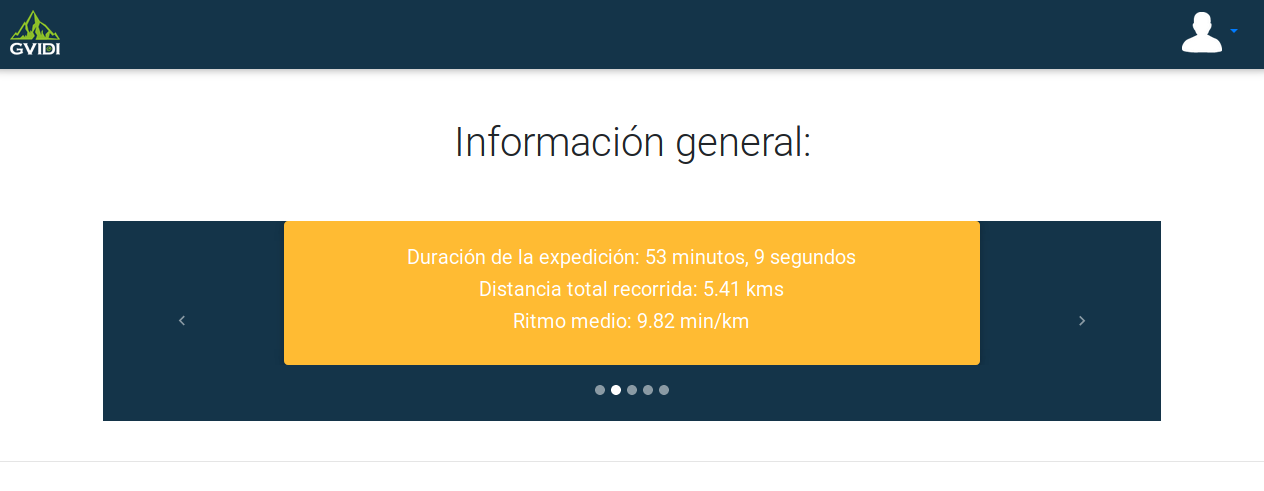
\includegraphics[width=0.8\textwidth]{infogeneral.png}
\caption{Tarjetas con información general acerca de la ruta.}
\label{fig:infogeneral}
\end{figure}

\begin{figure}
\centering
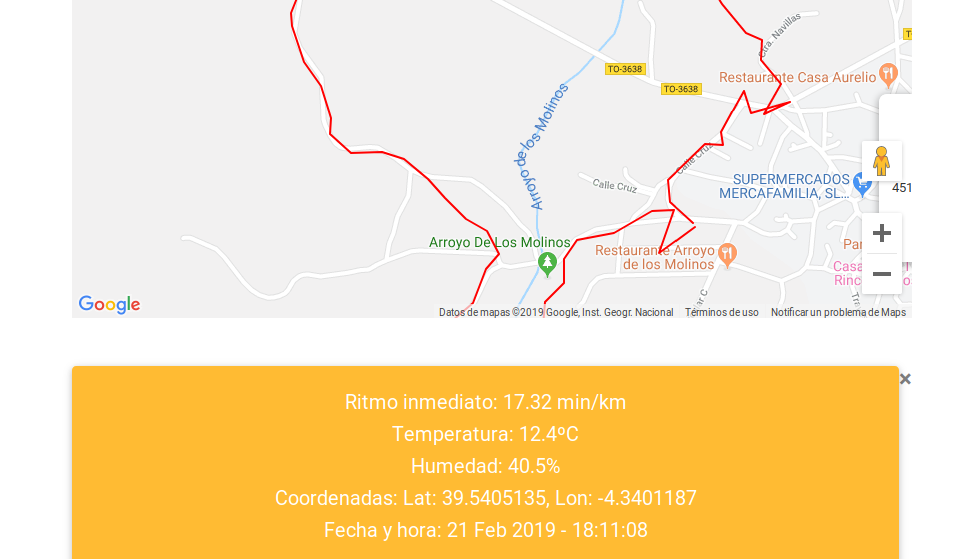
\includegraphics[width=0.8\textwidth]{mapainfo.png}}
\caption{Mapa en tiempo real de la expedición con información detallada del punto en el que se haga \textit{click}.}
\label{fig:mapainfo}
\end{figure}

Se realizó una primera versión de la plataforma \textit{web} en la que toda la lógica de gestión de usuarios y recuperación de datos de expediciones se hacía en el \textit{frontend}, implementada en los propios componentes \texttt{React}. El componente \texttt{React} de inicio de sesión, gestionaba por ejemplo la autenticación de un usuario, recuperando los datos de la vista, realizando la conexión con el sistema de autenticación de \texttt{Firebase} y alterando el estado del componente con el resultado de la autenticación.

Se obtuvo una plataforma \textit{web} totalmente funcional, que cumplía con todos los objetivos propuestos pero claramente insegura. Las credenciales para la conexión con las \ac{API}s de \texttt{Firebase} y \texttt{Firestore} las gestionaba el \textit{frontend} por lo que cualquier usuario podría visualizarlas desde el propio navegador. La obtención de dichas credenciales por parte de terceras personas podría hacer que se borrasen usuarios de las bases de datos y se alterasen los valores de las expediciones, entre otras acciones maliciosas. 

Para remediarlo se decidió añadir el \textit{backend} usando \texttt{NodeJS}. Este \textit{backend} implementa una serie de controladores con funciones, con las que el \textit{frontend} interactúa a través de consultas \ac{HTTP}. La lógica de conexión con \texttt{Firestore} y \texttt{Firebase}, reside en el servidor por lo que el usuario no es capaz de consultar ningún tipo de credencial desde su navegador. Con esta solución, si un usuario quiere iniciar sesión, enviará una petición al servidor con los datos de autenticación para que sea este quien le autentique. El servidor simplemente responderá con un valor que indicará si la autenticación ha sido satisfactoria.

\subsection{Implementación de la plataforma \textit{web}}

Para la implementación de la plataforma \textit{web} se ha usado \texttt{Javascript} como lenguaje de programación tanto en el \textit{frontend} (con \texttt{React} como librería escrita en \texttt{Javascript}) como en el \textit{backend} (con \texttt{Node} como \textit{framework} escrito en \texttt{Javascript}). También se ha hecho uso del lenguaje de marcas \ac{HTML} para definir el esqueleto de las distintas páginas \textit{web} que conforman el \textit{frontend}. Aunque no se han programado estilos propios usando \ac{CSS}, se ha usado \texttt{Bootstrap} para definir los estilos de la vista, mediante uso de plantillas de diseño predefinidas que permiten un prototipado rápido de la \textit{web}.

\subsubsection{Servidor \texttt{Express}}

Para implementar la lógica del servidor se ha hecho uso de \texttt{Express}, un \textit{framework} usado para implementar aplicaciones \textit{web} en la parte del servidor usando \texttt{Node}. Este \textit{framework} proporciona una serie de características que permiten construir aplicaciones de una única página, multipágina e híbridas de una forma sencilla. La instalación de \texttt{Express} se realiza a través del gestor de paquetes de \texttt{node} (\ac{npm}). En el Listado \ref{lst:express} se puede observar la creación del servidor \texttt{Express}. Simplemente es necesario inicializar el módulo \texttt{Express}, establecer el puerto en el que el servidor escuchará las peticiones entrantes y establecer las rutas que el servidor gestionará (véase Listado \ref{lst:expRoutes}), con el controlador para cada una de las rutas (véase Listado \ref{lst:expController}), que será la función que se ejecutará cuando se haga una petición a dicha ruta (ya sea una petición \texttt{GET} o una petición \texttt{POST}).

\begin{lstlisting}[language=javascript,captionpos=t,caption={\textbf{Creación del servidor \texttt{Express} de la plataforma \textit{web}.}},label={lst:express}]
const express = require('express');
const http = require('http');

const app = express();
// El puerto por defecto del servidor es el 4000
app.set('port', process.env.PORT || 4000);

// Establecer las rutas a la api de usuarios (para interactuar con usuarios)
app.use('/api/users', require('./routes/UserRoutes'));
// Establecer las rutas a la api de expediciones
app.use('/api/expeditions', require('./routes/ExpeditionRoutes'));

var server_created = http.createServer(app).listen(app.settings.port, function() {
	console.log ('Server listening on port ' + app.settings.port);
});
\end{lstlisting}

\begin{lstlisting}[language=javascript,captionpos=t,caption={\textbf{Rutas que gestiona el servidor al manejar peticiones a la \ac{API} de expediciones.}},label={lst:expRoutes}]
const express = require('express');
const expeditionRouter = express.Router();

const expeditionController = require('../controllers/ExpeditionController');

expeditionRouter.get('/allexpeditions', expeditionController.GetExpeditionsFromUser);
expeditionRouter.get('/expedition', expeditionController.GetExpedition);
...

module.exports = expeditionRouter;
\end{lstlisting}

\begin{lstlisting}[language=javascript,captionpos=t,caption={\textbf{Controlador de expediciones, que gestiona la lógica de la petición.}},label={lst:expController}]
const firebase = require('firebase');

const expeditionController = {};

// Funcion que proporciona todas las expediciones de las que un usuario ha formado parte
expeditionController.GetExpeditionsFromUser = (req, res) => {
  const db = firebase.firestore();
  const expeditionsRef = db.collection('Expeditions');
  const current_user = firebase.auth().currentUser;
  let expeditions_array = [];

  if (current_user) {
    ...
    res.json(expeditions_array);
  }
};

module.exports = expeditionController;
\end{lstlisting}

Por tanto, como se puede ver en la Figura \ref{fig:backendArch} la lógica del \textit{backend} se puede resumir en el servidor de aplicación \texttt{Express} que gestiona las peticiones entrantes y salientes, la \ac{API} que queda definida por el conjunto de rutas a las que se puede acceder desde el exterior (desde el \textit{frontend} o incluso desde otra aplicación \textit{web}, siempre y cuando se exponga el servidor \textit{backend} a Internet) y por los controladores que implementan la lógica de la petición, es decir, de qué forma actuar ante las peticiones a la \ac{API}.

\subsubsection{Autenticación de usuarios en \texttt{Firebase} y almacenamiento de datos en \texttt{Firestore}} 

Al igual que ocurría con la aplicación móvil, se ha hecho uso de \texttt{Firebase} para el proceso de autenticación de usuarios y de \texttt{Firestore} como base de datos en tiempo real \texttt{NoSQL}. En este punto del proyecto es en el que realmente se reflejan los puntos fuertes de haber elegido estos servicios para gestionar la autenticación y gestión de datos ya que se ha ahorrado una cantidad de tiempo considerable con esta elección. Se han omitido las fases de diseño e implementación de una solución propia para la gestión de datos, además de las dificultades relacionadas con cerciorarse de que existen políticas de seguridad adecuadas para acceder a los datos. 

\texttt{Firebase} y \texttt{Firestore} proporcionan \ac{API}s en varios lenguajes de programación (entre los que se incluyen \texttt{Java} para la aplicación móvil y \texttt{Javascript} para la plataforma \textit{web}) lo que hace que el sistema de autenticación y de gestión de datos quede unificado en todo el proyecto.

\begin{figure}
\centering
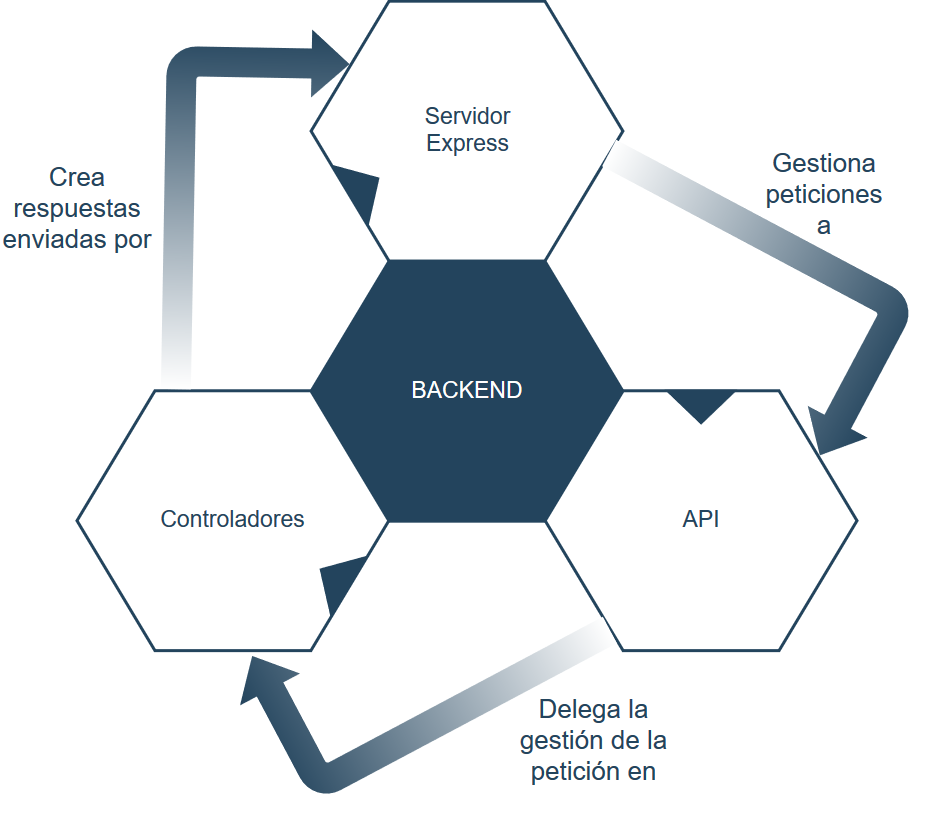
\includegraphics[width=0.6\textwidth]{backendArch.png}}
\caption{Esquema del \textit{backend} de la plataforma \textit{web}.}
\label{fig:backendArch}
\end{figure}

Para poder usar \texttt{Firebase} en la plataforma \textit{web} es necesario usar las mismas credenciales que las que se usaron para acceder a la \ac{API} de la aplicación móvil. En el Listado \ref{lst:firebaseWeb} se puede observar la sencillez en la conexión entre la plataforma \textit{web} y los servicios de \texttt{Firebase}. Una vez que se tienen las credenciales de la \ac{API}, solo es necesario importar el paquete de \texttt{Firebase} (que se puede instalar a través de \ac{npm}) e inicializar la aplicación. Este paquete contiene el \ac{SDK} para poder hacer uso de \texttt{Firebase} en el proyecto \textit{web}.

\begin{lstlisting}[language=javascript,captionpos=t,caption={\textbf{Creación de la conexión con \texttt{Firebase} en la aplicación \textit{web}.}},label={lst:firebaseWeb}]
const firebase = require('firebase')

const config = {
    apiKey: CLAVE_DE_LA_API,
    authDomain: 'ejemplo.firebaseapp.com',
    databaseURL: 'https://ejemplo.firebaseio.com"',
    storageBucket: 'ejemplo.appspot.com',
    projectId: 'ejemplo'
};

firebase.initializeApp(config);
\end{lstlisting}

Como \texttt{Firestore} es un servicio de almacenamiento de datos en tiempo real integrado dentro de \texttt{Firebase}, no es necesario usar credenciales distintas para acceder a los servicios de almacenamiento de datos. Una vez que se ha habilitado el uso de \texttt{Firestore} como sistema de gestión de datos desde la consola del proyecto de \texttt{Firebase}\footnote{\url{https://console.firebase.google.com}} (véase Figura \ref{fig:addfirestore}), se pueden realizar peticiones a la base de datos de una forma sencilla, como se puede ver en el Listado \ref{lst:firestoreJavascript}.


\begin{lstlisting}[language=javascript,captionpos=t,caption={\textbf{Consulta de los datos de todas las expediciones usando \texttt{Firestore} y \texttt{Javascript}.}},label={lst:firestoreJavascript}]
const db = firebase.firestore();
const expeditionsRef = db.collection('Expeditions');

expeditionsRef.get().then(querySnapshot => {
  querySnapshot.forEach(doc => {
    const data = doc.data();
  });
});
\end{lstlisting}

\begin{figure}
\centering
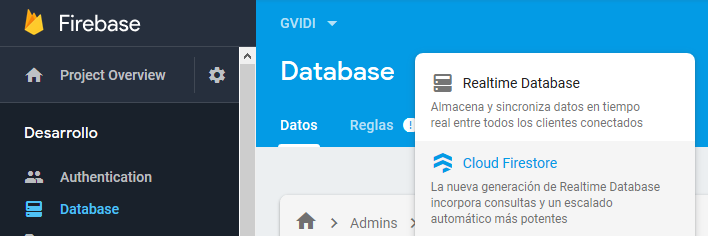
\includegraphics[width=0.9\textwidth]{addFirestore.png}}
\caption{Habilitar \texttt{Firestore} desde el proyecto de \texttt{Firebase}.}
\label{fig:addfirestore}
\end{figure}

\subsubsection{Mapa del recorrido}
\label{MapaRecorrido}

Para poder visualizar el recorrido que realiza un usuario en la expedición, se ha decidido añadir un mapa sobre el cual se irá dibujando, en forma de líneas, el camino que se realiza en la expedición (véase Figura \ref{fig:mapa_recorrido}). Además sobre el mapa se añadirán otros indicadores visuales, en forma de marcadores, para identificar las alertas que se han producido. \texttt{Google Maps} es la alternativa más contemplada en lo que al uso de mapas se refiere, ya que posee una \ac{API} para desarrolladores que permite explotar de diversas formas el uso de los mapas (en este proyecto se usará principalmente la creación de rutas o caminos sobre un mapa y la inserción y customización de marcadores en el mismo).

\begin{figure}
\centering
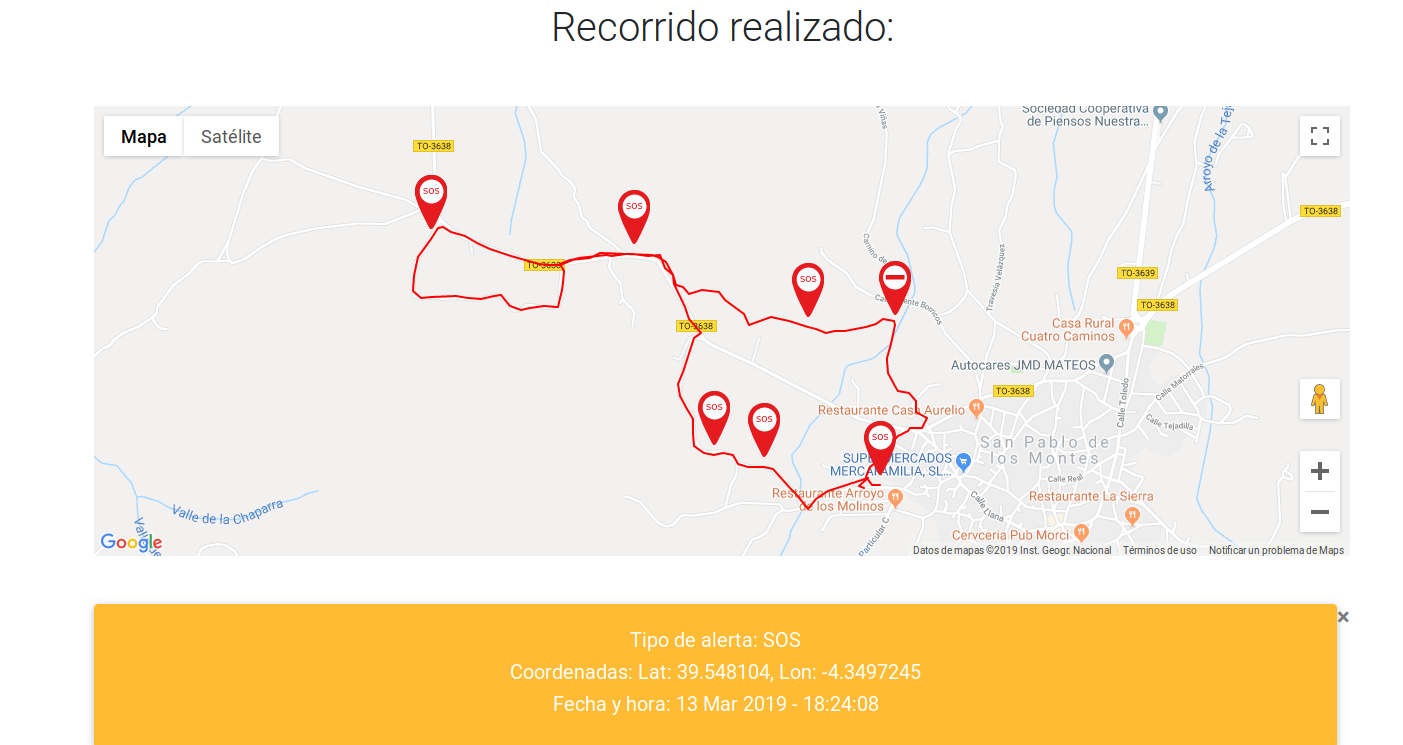
\includegraphics[width=0.9\textwidth]{mapa_durante_ruta.png}}
\caption{Mapa durante el recorrido de la expedición, en el que se pueden consultar detalles y alertas de dicha expedición.}
\label{fig:mapa_recorrido}
\end{figure}

Como se puede observar en la sección \ref{apiGoogleMaps} del antiguo capítulo de antecedentes, añadido en el presente proyecto en forma de anexo, lo único necesario para usar la \ac{API} de \texttt{Google Maps} en este proyecto es una <<\ac{API} \textit{Key}>>\footnote{\url{https://developers.google.com/maps/documentation/javascript/get-api-key}}. En el Listado \ref{lst:googlemapsweb} se puede observar la creación del mapa usando \texttt{React}. Además del mapa, también se crean los marcadores de las alertas de la ruta y la línea poligonal que dará lugar a la ruta por la que la expedición transcurre. Para que el usuario identifique de forma visual el tipo de alerta en la \textit{web}, se cambia la imagen del marcador dependiendo de la alerta.

\begin{lstlisting}[language=javascript,captionpos=t,caption={\textbf{Creación del mapa en la plataforma \textit{web}, incluyendo la ruta y los marcadores de alertas}.},label={lst:googlemapsweb}]
googleMapsAPI(API_CONFIG).then(googleMaps => {
  // Crear un nuevo mapa y establecer el punto central y el zoom
  let map = new googleMaps.Map(self.refs.map, { center: { lat: lat, lng: lng }, zoom: 16 });

   // Cada alerta es un marcador en el mapa
  self.state.alerts.forEach(alert => {
    let myLatlng = new googleMaps.LatLng(alert.Latitude, alert.Longitude);
    let image = undefined;
    // Depende del tipo de alerta, el marcador tendra un aspecto u otro
    if (alert.AlertType === 'STOP') {
      image = { url: window.location.origin + '/marker_stop_32.png', size: new googleMaps.Size(32, 64), origin: new googleMaps.Point(0, 0) }
    else if (alert.AlertType === 'SOS') {
      image = { url: window.location.origin + '/marker_sos_32.png', size: new googleMaps.Size(32, 64), origin: new googleMaps.Point(0, 0) }
    }
    let marker = new googleMaps.Marker({ position: myLatlng, animation: googleMaps.Animation.DROP, title: 'Alerta', icon: image });
    // Listener que se ejecutara cuando se hace click en un marcador
    marker.addListener('click', args => {
       ...
    });
    marker.setMap(map);
  });

  // Crear la linea de la ruta
  let poli = new googleMaps.Polyline({
    path: self.state.locations,
    geodesic: true,
    strokeColor: '#FF0000',
    strokeOpacity: 1.0,
    strokeWeight: 2
  });

  poli.setMap(map);

  // Listener que se ejecutara cuando se hace click en la ruta
  poli.addListener('click', args => {
    ...
  });
});
\end{lstlisting}

Cuando el usuario pulsa un marcador, debajo del mapa aparece una tarjeta con información detallada acerca de la alerta. De igual forma, cuando el usuario pulsa sobre un punto en la ruta del mapa, se busca el instante más cercano al punto seleccionado en el cual se tienen datos de la expedición y se muestra una tarjeta debajo del mapa con información detallada acerca de la expedición en ese instante. 

La aplicación móvil almacena una nueva entrada con datos relativos a la posición del usuario en la expedición cada veinte segundos, por lo que es muy probable que las coordenadas elegidas por el usuario cuando pulsa un punto en la ruta del mapa no dispongan de información para ese mismo instante. Lo que se hace en este caso es buscar el punto más cercano a las coordenadas elegidas por el usuario del que se dispone información y mostrar la información de ese punto. Esto no es ningún problema, ya que si se pulsa un punto en la ruta durante el transcurso normal de la expedición se verá la información del punto más cercano a las coordenadas seleccionadas del que se disponen datos y como el período de envío de datos de localización es tan alto (cada veinte segundos) el usuario no notará una falta de información en ningún momento. Si se produce una alerta las coordenadas que se muestran si que son las exactas de la alerta, ya que en caso de caída se requiere la máxima precisión posible para identificar el lugar de la caída.

En el Listado \ref{lst:getminlocation} se puede observar el algoritmo que implementa la funcionalidad que se acaba de explicar y en el Listado \ref{lst:harvesineformula} se encuentra el algoritmo necesario para calcular la distancia entre dos puntos. Este algoritmo está basado en la fórmula de \textit{Harvesine}, que calcula la distancia ortodrómica o mínima distancia entre dos puntos en la superficie terrestre (véase Figura \ref{fig:ortodroma}), sabiendo sus longitudes y latitudes. La fórmula de \textit{Harvesine} es la siguiente:

\begin{equation}
d = 2\cdot r \cdot \arcsin{\left( \sqrt{\sin^2\left(\frac{\phi_2 - \phi_1}{2} \right) + \cos \left( \phi_1 \right) \cdot \cos \left( \phi_2 \right) \cdot \sin^2 \left( \frac{\lambda_2 - \lambda_1}{2} \right)}\right)}
\end{equation}

donde $\phi_1, \lambda_1$ se refiere a la latitud y longitud del primer punto, $\phi_2, \lambda_2$ se refiere a la latitud y longitud del segundo punto y $r$ se refiere al radio de la circunferencia que engloba los puntos (en este caso, el radio terrestre).

\begin{lstlisting}[language=javascript,captionpos=t,caption={\textbf{Obtención de la localización más cercana a un punto dado}.},label={lst:getminlocation}]
expeditionController.GetMinLocation = (req, res) => {
  const db = firebase.firestore();
  const expeditionsRef = db.collection('Expeditions');

  let expeditionName = req.query.expName;
  let lat = req.query.lat;
  let lon = req.query.lon;
  let min_distance = Infinity;
  let min_location = null;

  expeditionsRef.get().then(querySnapshot => {
    querySnapshot.forEach(doc => {
      const data = doc.data();
      if (data.ExpName === expeditionName) {
        data.Guide.PreviousLocations.forEach(location => {
          let distance = getDistanceBetweenTwoPoints(lat, lon, parseFloat(location.Lat), parseFloat(location.Lon));
          if (distance < min_distance) {
            min_distance = distance;
            min_location = location;
          }
        });
      }
    });
  });
};
\end{lstlisting}

\begin{figure}
    \centering
    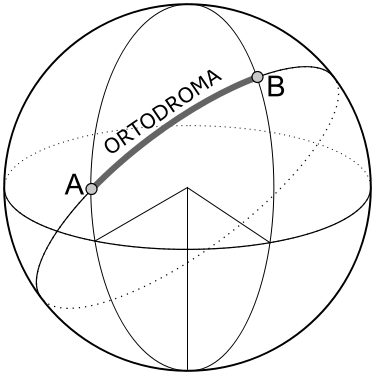
\includegraphics[width=0.4\textwidth]{otrodroma.png}
    \caption{Distancia ortodrómica entre dos puntos sobre la superficie de una esfera. \protect\footnotemark}
    \label{fig:ortodroma}
\end{figure}

\footnotetext{Imagen extraída de \url{https://upload.wikimedia.org/wikipedia/commons/thumb/c/c2/Ortodroma.svg/375px-Ortodroma.svg.png}}

\begin{lstlisting}[language=javascript,captionpos=t,caption={\textbf{Obtención de la distancia entre dos puntos usando la formula de \textit{Harvesine}.}},label={lst:harvesineformula}]
function getDistanceBetweenTwoPoints(lat_first, lon_first, lat_second, lon_second) {
  lat_first = toRadians(Math.abs(lat_first));
  lon_first = toRadians(Math.abs(lon_first));
  lat_second = toRadians(Math.abs(lat_second));
  lon_second = toRadians(Math.abs(lon_second));

  let lat_distance = lat_first - lat_second;
  let lon_distance = lon_first - lon_second;

  let a = Math.pow(Math.sin(lat_distance / 2), 2) + Math.cos(lat_second) * Math.cos(lat_first) * Math.pow(Math.sin(lon_distance / 2), 2);
  let c = 2 * Math.atan2(Math.sqrt(a), Math.sqrt(1 - a));

  // El valor 6373.0 es el radio de la tierra
  return 6373.0 * c;
}
\end{lstlisting}

\section{Organización del proyecto en paquetes de trabajo}

Para la consecución del presente proyecto se definen un total de cuatro \ac{PT}, cada uno de los cuales está dividido en una serie de \ac{T}. En el diagrama de Gantt de la Figura \ref{fig:gantt}, se puede observar la descomposición temporal del proyecto en paquetes de trabajo y tareas.

\begin{landscape}
\begin{figure}[!h]
\begin{center}
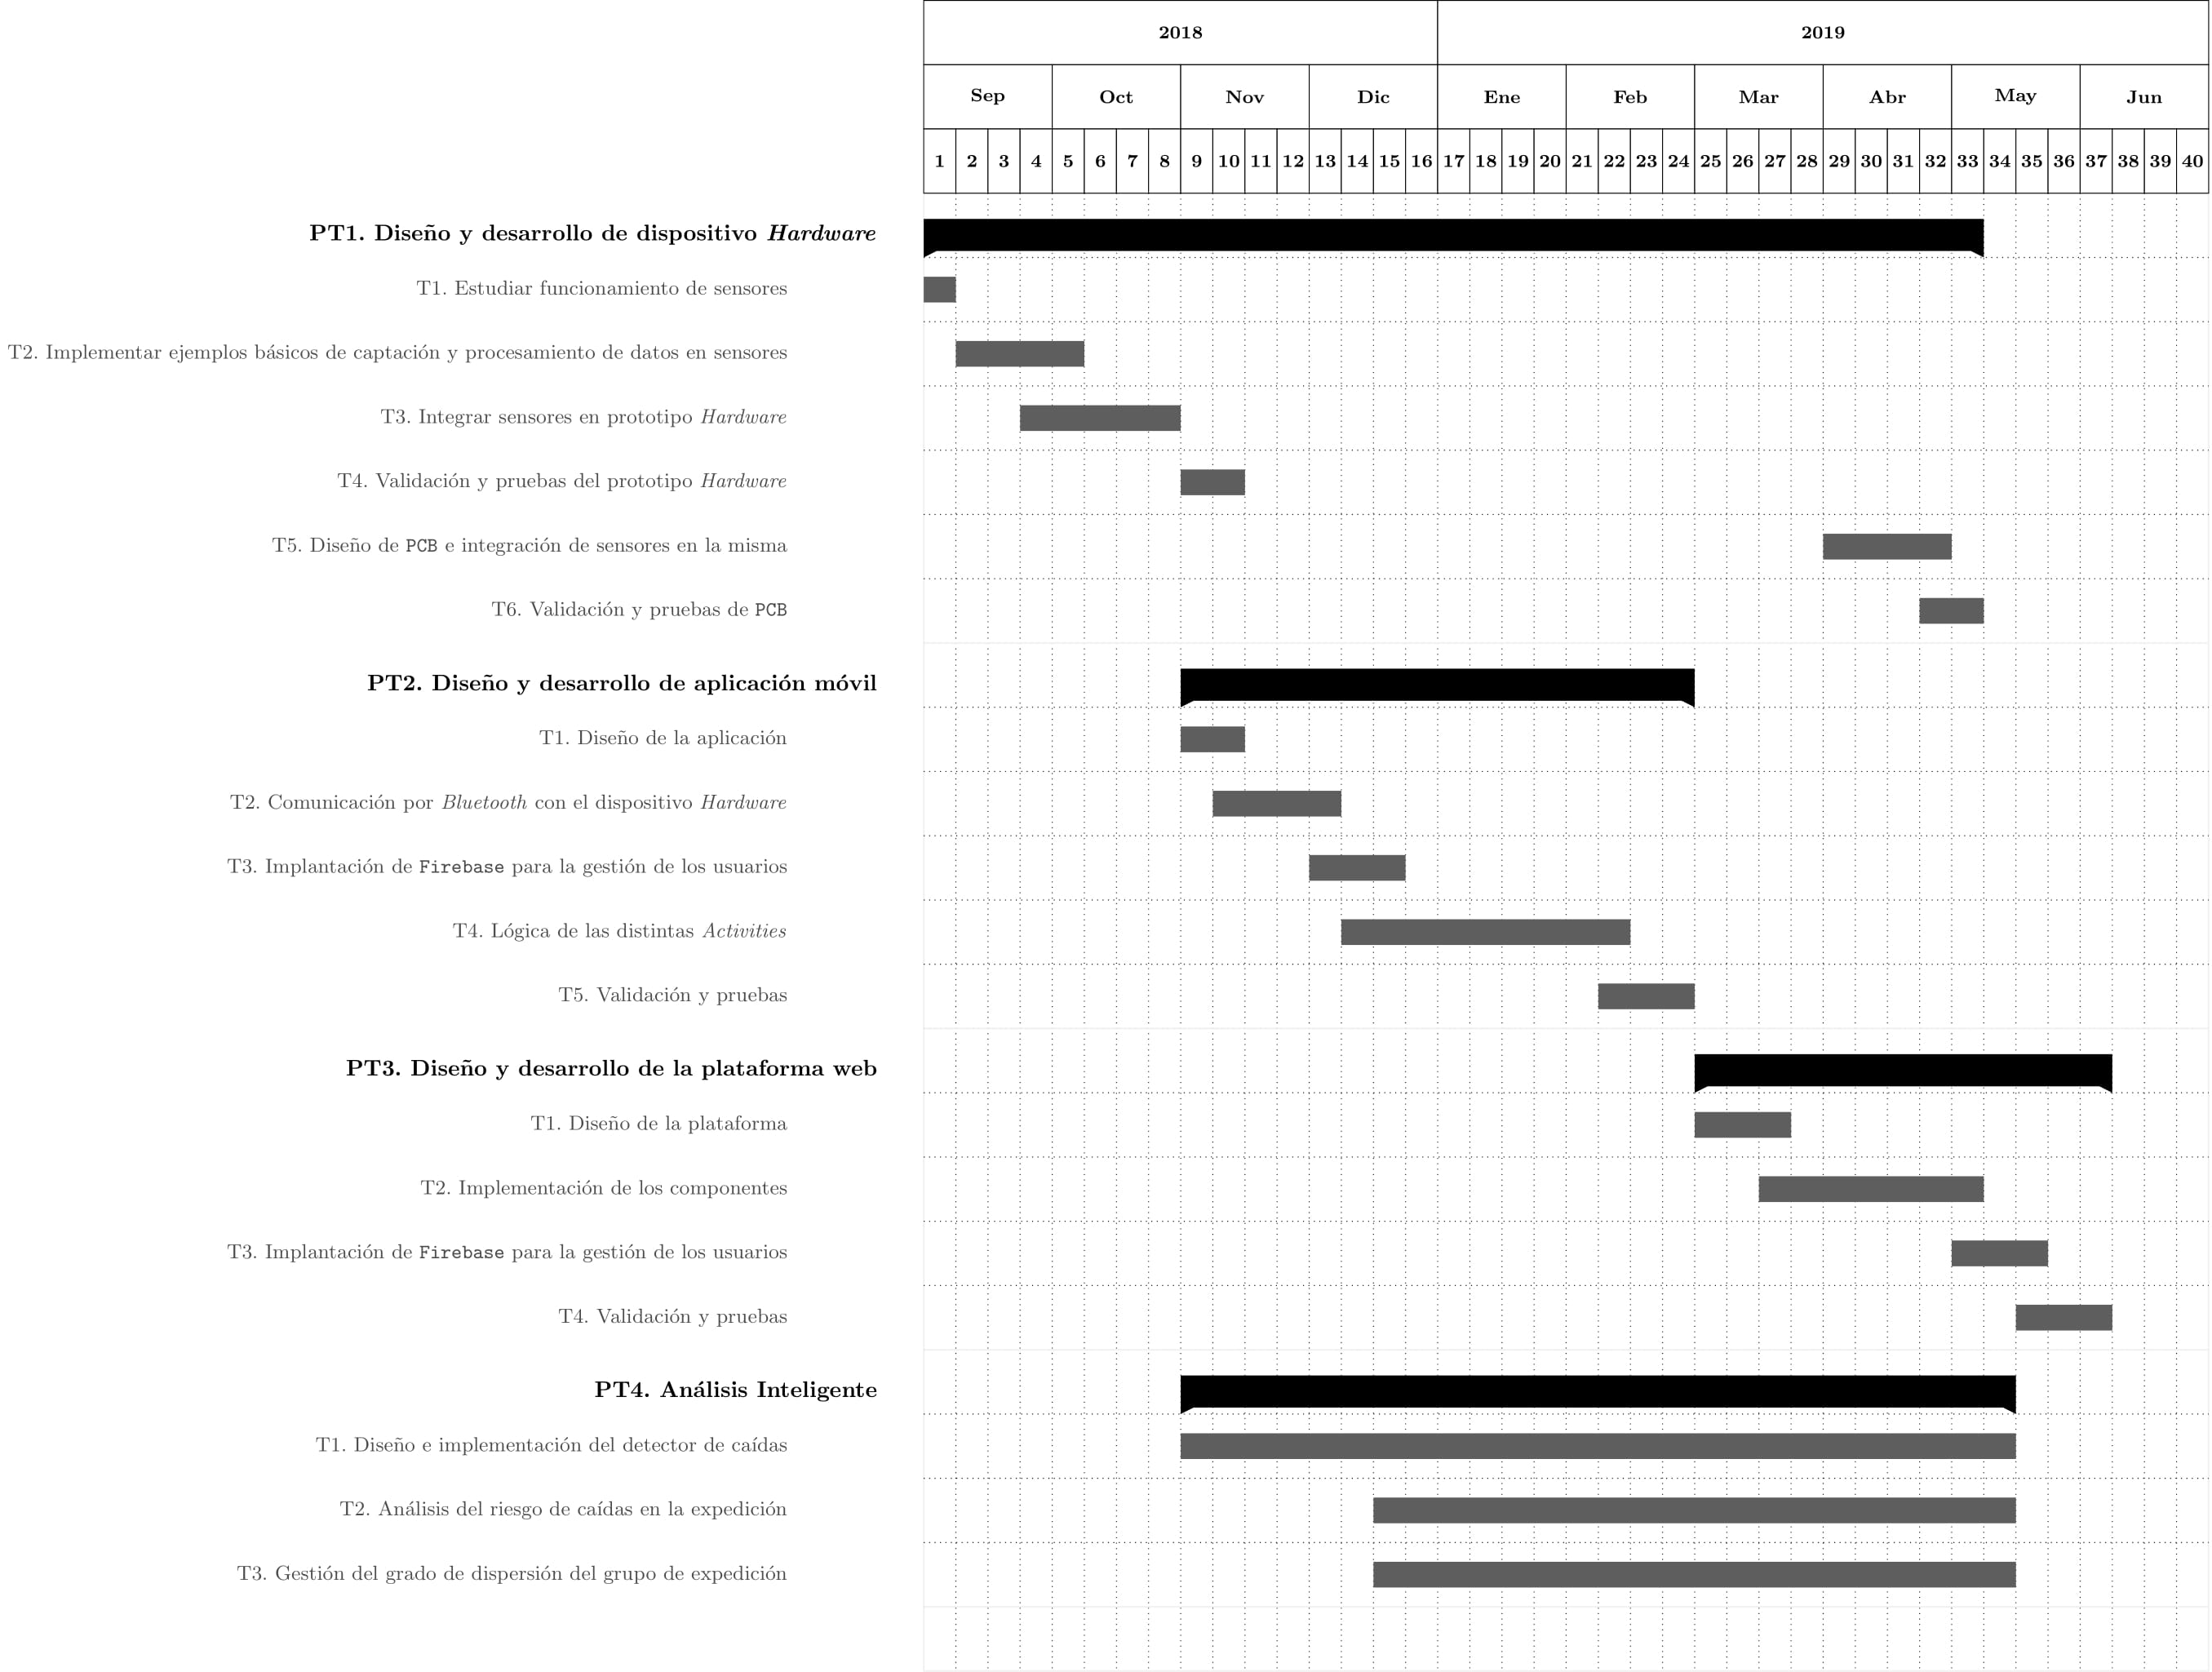
\includegraphics[width=1.5\textwidth]{Gantt_Char.jpg}
\caption{Diagrama de Gantt.}
\label{fig:gantt}
\end{center}
\end{figure}
\end{landscape}

\subsection{\ac{PT}1. Diseño y desarrollo de dispositivo \textit{Hardware} (Semanas 1 a 33)}

Este paquete de trabajo engloba todo lo relacionado con el dispositivo físico, con el principal objetivo de obtener un prototipo del dispositivo \textit{hardware} capaz de tomar los datos de los sensores necesarios y enviarlos a un dispositivo móvil, por medio de \textit{Bluetooth}. El trabajo en las tareas que conforman este paquete comenzó en la primera semana del proyecto y comprendió hasta la semana 33. Se obtuvo una versión del prototipo válida en la semana 10, pero semanas mas tarde se diseño la \ac{PCB} en la que se integraron los sensores del dispositivo, mejorando el diseño del prototipo final. 

El \ac{PT}1 se compone de las siguientes tareas:

\begin{itemize}
\item \textbf{\ac{T}1 (Semana 1). Estudiar funcionamiento de sensores.} Esta tarea está diseñada para conocer de forma más profunda los sensores que se van a manejar en el proyecto. Es una tarea importante ya que conocer el funcionamiento de los sensores hace más sencilla la interpretación de los valores de los mismos, así como la identificación de un posible comportamiento anómalo, en un momento dado. 
\item \textbf{\ac{T}2 (Semanas 2 a 5). Implementar ejemplos básicos de captación y procesamiento de datos en sensores.} A lo largo de esta tarea se realizaron varios ejemplos de código en los que se utilizaban los sensores de forma individual (captación de datos en el caso de sensores de temperatura, humedad y acelaración entre otros, y emisión de datos en el caso del módulo \textit{Bluetooth}). En esta tarea se realizó la búsqueda de librerías existentes que gestionasen los sensores o se implementaron librerías propias para los sensores que no tuviesen librerías disponibles.
\item \textbf{\ac{T}3 (Semanas 4 a 8). Integrar sensores en prototipo \textit{Hardware}}. Durante esta tarea se tomaron todos los ejemplos individuales de uso de sensores de la tarea anterior y se creó un solo \textit{sketch} que integraba todos los sensores.
\item \textbf{\ac{T}4 (Semanas 9 y 10). Validación y pruebas del prototipo \textit{Hardware}}. Esta tarea sirvió para identificar los fallos en el prototipo \textit{hardware} y corregirlos, obteniendo una versión estable del mismo.
\item \textbf{\ac{T}5 (Semanas 29 a 32). Diseño de \ac{PCB} e integración de sensores en la misma.} Durante esta tarea se diseñó y se construyó la \ac{PCB} (por una empresa que se dedica a la impresión de \ac{PCB}s) y se procedió a soldar todos los sensores en la misma. 
\item \textbf{\ac{T}6 (Semanas 31 a 33). Validación y pruebas de \ac{PCB}.} A lo largo de esta tarea se realizaron pruebas para cerciorarse de la correcta conexión de los sensores en la \ac{PCB}, del correcto diseño de la \ac{PCB} y del correcto funcionamiento del prototipo \textit{hardware}.
\end{itemize}

El resultado obtenido del \ac{PT}1 es la creación de un dispositivo \textit{hardware} equipado con sus correspondientes sensores que sea capaz de tomar datos de los mismos y comunicarlos a un dispositivo móvil a través de \textit{Bluetooth}.

\subsection{\ac{PT}2. Diseño y desarrollo de aplicación móvil (Semanas 9 a 24)}

Este paquete de trabajo tiene como responsabilidad el diseño y desarrollo de una aplicación móvil que tome datos de un microcontrolador a través de \textit{Bluetooth} y muestre información de manera amigable a los usuario de la misma.

El \ac{PT}2 está compuesto por las siguientes tareas:

\begin{itemize}
\item \textbf{\ac{T}1 (Semanas 9 y 10). Diseño de la aplicación.} A lo largo de esta tarea se realizaron los bocetos que darían lugar a las distintas pantallas de las que se compone la aplicación. Durante esta tarea también se llevó a cabo el diseño de la arquitectura \ac{MVC} de la aplicación móvil.
\item \textbf{\ac{T}2 (Semanas 10 a 13). Comunicación por \textit{Bluetooth} con el dispositivo \textit{Hardware}.} Durante esta tarea se llevó a cabo la conexión de la aplicación móvil con el dispositivo físico, usando el protocolo de comunicación inalámbrico \textit{Bluetooth}. Se desarrollaron distintas implementaciones de esta conexión hasta que se obtuvo una implementación que cumplía con una frecuencia de lectura de datos suficiente para realizar la detección de caídas.
\item \textbf{\ac{T}3 (Semanas 13 a 15). Implantación de \texttt{Firebase} para la gestión de los usuarios.} En esta tarea se realizó la creación y autenticación de usuarios en la aplicación móvil. También se realizó la conexión con la base de datos en tiempo real \texttt{Firestore} para almacenar los datos relacionados con las expediciones.
\item \textbf{\ac{T}4 (Semanas 14 a 22). Lógica de las distintas \textit{Activities}.} A lo largo de esta tarea se realizó la implementación de las actividades que conforman la aplicación móvil. Esta implementación no incluye el análisis inteligente de los datos, que comprende un paquete de trabajo completo.
\item \textbf{\ac{T}5 (Semanas 22 a 24). Validación y pruebas.} Durante esta tarea se llevaron a cabo una serie de pruebas de la aplicación móvil, para identificar los fallos de implementación en la misma y corregirlos.
\end{itemize}

El resultado obtenido del \ac{PT}2 es una aplicación móvil para el sistema operativo \textit{Android}, que tome datos de un microcontrolador a través de \textit{Bluetooth} y muestre información de manera amigable a los usuario de la misma.

\subsection{\ac{PT}3. Diseño y desarrollo de la plataforma \textit{web} (Semanas 25 a 37)}

Este paquete de trabajo tiene como responsabilidad el diseño y desarrollo de una plataforma \textit{web} que se encargue de mostrar información al usuario en tiempo real de la expedición que está realizando. De la misma manera, se encargará de mostrar un histórico de expediciones realizadas por el usuario, con los datos de las mismas.

El \ac{PT}3 se compone de las siguientes tareas:

\begin{itemize}
\item \textbf{\ac{T}1 (Semanas 25 a 27). Diseño de la plataforma.} Durante esta tarea se llevó a cabo la realización de bocetos que darían lugar a las distintas páginas de las que se compone la plataforma \textit{web}. En esta tarea también se definió la arquitectura que se ha usado al implementar la plataforma.
\item \textbf{\ac{T}2 (Semanas 27 a 33). Implementación de los componentes.} Esta tarea está diseñada para llevar a cabo la codificación de los distintos componentes \texttt{React} que conforman el \textit{frontend} de la plataforma. 
\item \textbf{\ac{T}3 (Semanas 33 a 35). Implantación de \texttt{Firebase} para la gestión de los usuarios.} A lo largo de esta tarea se llevó a cabo la autenticación y gestión de los usuarios en la plataforma \textit{web}. En esta tarea también se desarrolló el servidor \texttt{Express} y los distintos controladores del \textit{backend}.
\item \textbf{\ac{T}4 (Semanas 35 a 37). Validación y pruebas.} Durante esta tarea se llevaron a cabo una serie de pruebas de la plataforma \textit{web}, para identificar los fallos de implementación en la misma y corregirlos.
\end{itemize}

El resultado obtenido del \ac{PT}3 es una plataforma \textit{web}, usando \texttt{React} y \texttt{Node} como bibliotecas y \textit{frameworks} de desarrollo, que sirve para visualizar (en tiempo real y de forma histórica) información avanzada acerca de una expedición de la que el usuario ha tomado o esta tomando parte.

\subsection{\ac{PT}4. Análisis Inteligente(Semanas 9 a 34)}

Este paquete de trabajo tiene como responsabilidad la realización de un análisis inteligente a partir de los datos recogidos por los sensores del dispositivo físico (y otros datos captados gracias al dispositivo móvil). Este análisis inteligente es realizado por la aplicación móvil.

El \ac{PT}4 se compone de las siguientes tareas:

\begin{itemize}
\item \textbf{\ac{T}1 (Semanas 9 a 34). Diseño e implementación del detector de caídas.} Esta tarea sirvió para diseñar y desarrollar un algoritmo de detección de caídas usando datos de aceleración, siguiendo un enfoque basado en límites o umbrales. Durante esta tarea se realizaron pruebas con distintos valores de umbrales para conseguir minimizar los falsos positivos y falsos negativos. 
\item \textbf{\ac{T}2 (Semanas 15 a 34). Análisis del riesgo de caídas en la expedición.} A lo largo de esta tarea se realizó un algoritmo que utiliza lógica difusa para, a través de unos valores de entrada proporcionados por los sensores del dispositivo físico, inferir un grado de riesgo de caída en la expedición.
\item \textbf{\ac{T}3 (Semanas 15 a 34). Gestión del grado de dispersión del grupo de expedición.} Durante esta tarea se realizó un algoritmo que analiza el grado de dispersión de los usuarios de la expedición con respecto al guía, para prevenir posibles situaciones de riesgo en la expedición.
\end{itemize}

Los resultados obtenidos del \ac{PT}4 han sido una serie de algoritmos implementados en la aplicación móvil con el objetivo común de mejorar la seguridad de los usuarios en una expedición y ayudar al guía proporcionándole una mayor visión de la expedición en todo momento.

\section{Metodología de trabajo}

Para el desarrollo del proyecto, se ha optado por seguir una metodología basada en un desarrollo iterativo e incremental \cite{5} ya que esta metodología se adaptaba perfectamente a este proyecto. Para llevarlo a cabo, se han seguido una secuencia de pasos no lineales haciendo que cada poco tiempo se tenga una versión operativa del producto final. En este \ac{TFG} es muy importante esta característica, ya que era necesario tener una versión operativa del \textit{hardware} usado y el \textit{firmware} para la comunicación con el dispositivo físico antes de comenzar con otras fases como el análisis inteligente. Las posteriores iteraciones se han usado para, prioritariamente, corregir fallos de iteraciones anteriores. En nuevas iteraciones también se han añadido funcionalidades nuevas, aumentando la calidad del producto final. Al final de cada iteración se ha mantenido una reunión con el director del proyecto, que ha identificado fallos en el trabajo realizado hasta el momento, ha propuesto mejoras sobre el trabajo existente y nuevas funcionalidades a añadir.

El desarrollo del proyecto ha estado motivado por una metodología ágil \cite{6}. Cada iteración se ha dividido en una lista de tareas, a las que se les ha dado una prioridad antes de comenzar la iteración. Estas tareas han sido de corta duración (de una a cuatro semanas, a lo sumo), motivadas por la entrega de \textit{software} funcional y que aporta valor. La comunicación con el director del proyecto ha sido continua durante la ejecución de las tareas. Durante los primeros meses del proyecto se mantuvieron reuniones presenciales con el director del mismo cada semana (o a lo sumo cada dos semanas). Durante los meses finales las reuniones fueron a través de videoconferencia cada dos semanas o cuando se encontraba alguna dificultad en la consecución del proyecto. Se ha usado un método basado en un tablero \textit{Kanban} para gestionar el tiempo y visualizar en todo momento qué tareas de la iteración se han realizado y cuáles faltan por realizar (ver Figura \ref{fig:trello}).

También se ha usado \texttt{git} como sistema de control de versiones, para mantener un registro detallado de qué cambios se realizan en cada uno de los archivos del repositorio creado para este proyecto. El repositorio \texttt{git} se ha alojado en \texttt{GitHub}, como se puede observar en la Figura \ref{fig:githubgvidi}. 

\begin{figure}[!h]
\begin{center}
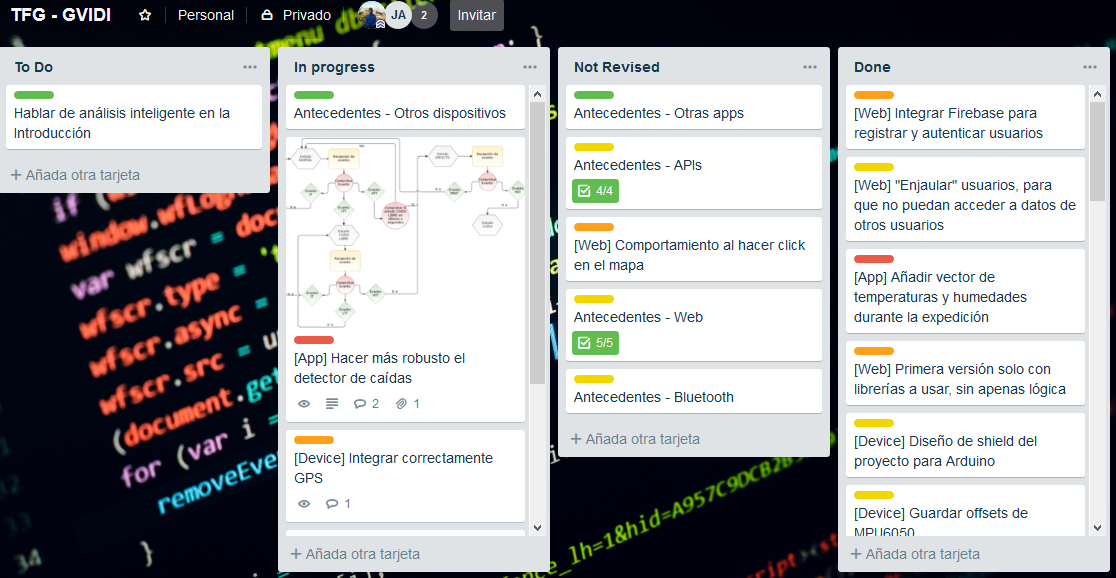
\includegraphics[width=0.75\textwidth]{trello.png}
\caption{Tablero de \texttt{Trello}\footnote{\url{https://www.trello.com}} usado durante el \ac{TFG}.}
\label{fig:trello}
\end{center}
\end{figure}

\begin{figure}[!h]
\begin{center}
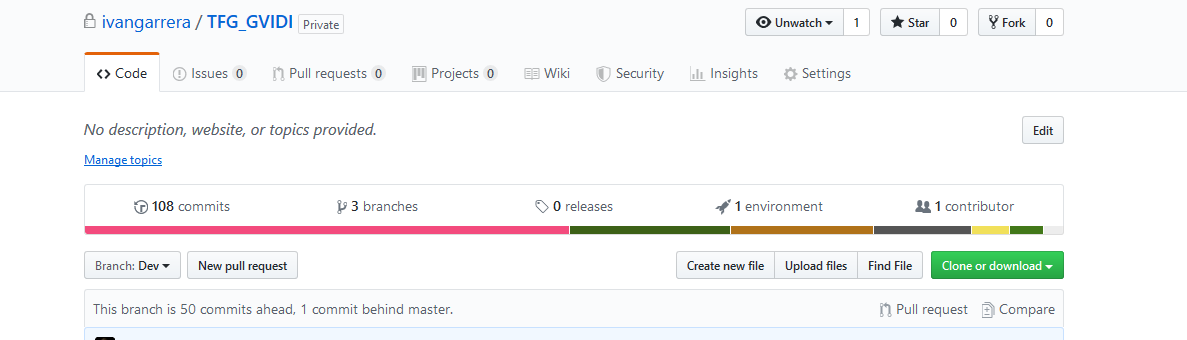
\includegraphics[width=0.6\textwidth]{githubgvidi.png}
\caption{Repositorio \texttt{git} del proyecto, alojado en \texttt{GitHub}.\footnote{\url{https://github.com}}}
\label{fig:githubgvidi}
\end{center}
\end{figure}


\subsection{Iteraciones}

Este proyecto está compuesto por un total de diez iteraciones. Las primeras iteraciones se centran en el análisis del alcance del proyecto, la recogida de requisitos y la búsqueda del \textit{hardware} necesario para construir un prototipo del dispositivo \textit{hardware}. A continuación, las iteraciones se centran en la mejora del prototipo \textit{hardware}, el diseño y desarrollo de la aplicación móvil y la redacción del capítulo de antecedentes del presente \ac{TFG}. Las últimas iteraciones se centran en las pruebas de la aplicación móvil, el diseño y creación de la \ac{PCB} para mejorar el dispositivo físico, el diseño, desarrollo y pruebas de la plataforma \textit{web} y la redacción de esta memoria. A continuación se van a detallar cada una de las diez iteraciones que se han realizado:

\subsubsection{Iteración 1}

\begin{table}[!h]
\centering
\begin{tabular}{|l|l|l|l|l|c|}
\hline
\rowcolor[HTML]{343434} 
\multicolumn{1}{|c|}{\cellcolor[HTML]{343434}{\color[HTML]{FFFFFF} \textbf{\begin{tabular}[c]{@{}c@{}}Paquetes de\\ Trabajo\end{tabular}}}} & \multicolumn{1}{c|}{\cellcolor[HTML]{343434}{\color[HTML]{FFFFFF} \textbf{\begin{tabular}[c]{@{}c@{}}Tareas a las\\ que afecta\end{tabular}}}} & \multicolumn{1}{c|}{\cellcolor[HTML]{343434}{\color[HTML]{FFFFFF} \textbf{\begin{tabular}[c]{@{}c@{}}Objetivos\\ alcanzados\end{tabular}}}}                            & \multicolumn{1}{c|}{\cellcolor[HTML]{343434}{\color[HTML]{FFFFFF} \textbf{\begin{tabular}[c]{@{}c@{}}Fecha\\ Inicio\end{tabular}}}} & \multicolumn{1}{c|}{\cellcolor[HTML]{343434}{\color[HTML]{FFFFFF} \textbf{\begin{tabular}[c]{@{}c@{}}Fecha\\ Fin\end{tabular}}}} & \multicolumn{1}{c|}{\cellcolor[HTML]{343434}{\color[HTML]{FFFFFF} \textbf{\begin{tabular}[c]{@{}c@{}}Tiempo\\ Estimado\end{tabular}}}} \\ \hline
\rowcolor[HTML]{EFEFEF} 
{\color[HTML]{000000} Documentación}                                                                                                        & {\color[HTML]{000000} }                                                                                                                        & {\color[HTML]{000000} \begin{tabular}[c]{@{}l@{}}- Recogida de\\ requisitos\\ - Definición del\\ alcance del proyecto\\ - Realización del\\ anteproyecto\end{tabular}} & {\color[HTML]{000000} \begin{tabular}[c]{@{}l@{}}01/08/\\ 2018\end{tabular}}                                                        & {\color[HTML]{000000} \begin{tabular}[c]{@{}l@{}}31/08/\\ 2018\end{tabular}}                                                     & {\color[HTML]{000000} 30h}                                                                                                             \\ \hline
\end{tabular}
\caption{Descripción resumida de la primera iteración.}
\end{table}

En esta iteración se llevaron a cabo las tareas relacionadas con la recogida de requisitos, para definir qué detalles específicos se van a llevar a cabo durante la consecución del proyecto. Una vez recogidos los requisitos se definió el alcance del proyecto, para tener una idea del tiempo y los recursos que se emplearían. Durante esta iteración también se llevó a cabo la realización del anteproyecto.

Los requisitos que se obtuvieron fueron:

\begin{itemize}
\item El dispositivo \textit{hardware} será capaz de obtener datos de los sensores necesarios y los enviará a un dispositivo móvil por \textit{Bluetooth}.
\item El dispositivo \textit{hardware} debe estar equipado con botones físicos para generar alertas.
\item Se diseñará una \ac{PCB} para mejorar el prototipo \textit{hardware}.
\item La aplicación móvil se realizará usando el sistema operativo \texttt{Android}.
\item La aplicación móvil será capaz de recibir los datos provenientes del microcontrolador por medio de \textit{Bluetooth}.
\item La aplicación móvil debe proporcionar información distinta y relevante para guías y para participantes de las distintas expediciones.
\item Tanto el guía como los participantes deben poder visualizar en un mapa su situación en el grupo de expedición.
\item El dispositivo móvil será capaz de usar la información proveniente del microcontrolador para detectar caídas en los miembros y guía del grupo de expedición.
\item El dispositivo móvil debe inferir un grado de peligrosidad usando la información de los sensores, que el guía y los participantes pueden usar para maximizar su precaución.
\item El dispositivo móvil le proporcionará al guía información sobre la distancia a la que se encuentran los participantes de la expedición, así como información sobre el grado de dispersión del grupo.
\item La autenticación en la aplicación móvil y en la plataforma \textit{web} se realizará usando \texttt{Firebase}, para maximizar la seguridad durante el proceso de autenticación.
\item La plataforma \textit{web} tendrá un diseño \textit{responsive}, que se adaptará al tamaño de pantalla del dispositivo dónde se visualice.
\item La plataforma \textit{web} mantendrá un histórico de todas las expediciones en las que ha tomado parte un determinado participante o guía, con información relevante sobre ellas.
\item Debe ser posible que una persona autorizada por el participante en la expedición pueda seguir en tiempo real el transcurso de la misma.
\end{itemize}

\subsubsection{Iteración 2}

\begin{table}[!h]
\centering
\begin{tabular}{|c|c|l|l|l|c|}
\hline
\rowcolor[HTML]{343434} 
{\color[HTML]{FFFFFF} \textbf{\begin{tabular}[c]{@{}c@{}}Paquetes de\\ Trabajo\end{tabular}}} & {\color[HTML]{FFFFFF} \textbf{\begin{tabular}[c]{@{}c@{}}Tareas a las\\ que afecta\end{tabular}}} & \multicolumn{1}{c|}{\cellcolor[HTML]{343434}{\color[HTML]{FFFFFF} \textbf{\begin{tabular}[c]{@{}c@{}}Objetivos\\ alcanzados\end{tabular}}}}                                                           & \multicolumn{1}{c|}{\cellcolor[HTML]{343434}{\color[HTML]{FFFFFF} \textbf{\begin{tabular}[c]{@{}c@{}}Fecha\\ Inicio\end{tabular}}}} & \multicolumn{1}{c|}{\cellcolor[HTML]{343434}{\color[HTML]{FFFFFF} \textbf{\begin{tabular}[c]{@{}c@{}}Fecha\\ Fin\end{tabular}}}} & {\color[HTML]{FFFFFF} \textbf{\begin{tabular}[c]{@{}c@{}}Tiempo\\ Estimado\end{tabular}}} \\ \hline
\rowcolor[HTML]{EFEFEF} 
{\color[HTML]{000000} \ac{PT}1}                                                               & {\color[HTML]{000000} \ac{T}1,\ac{T}2,\ac{T}3}                                                    & {\color[HTML]{000000} \begin{tabular}[c]{@{}l@{}}- Compra de\\ componentes que\\ conformarían el\\ dispositivo físico\\ - Búsqueda o \\ realización de \\ librerías para los\\ sensores\end{tabular}} & {\color[HTML]{000000} \begin{tabular}[c]{@{}l@{}}02/09/\\ 2018\end{tabular}}                                                        & {\color[HTML]{000000} \begin{tabular}[c]{@{}l@{}}28/10/\\ 2018\end{tabular}}                                                     & {\color[HTML]{000000} 35h}                                                                \\ \hline
\end{tabular}
\caption{Descripción resumida de la segunda iteración.}
\end{table}

Durante esta iteración se realizó una búsqueda de todos los sensores que se necesitarían en el proyecto (véase Tabla \ref{table:componentes}) y se procedió a la compra de los mismos gracias al grupo de investigación \texttt{AIR}\footnote{\url{http://air.esi.uclm.es/}}. Después de estudiar distintas alternativas en lo que a los microcontroladores se refiere (por ejemplo \texttt{Raspberry Pi}, \texttt{STM32} o \texttt{Arduino}), finalmente se eligió el último de los nombrados por la rapidez de prototipación, la gran disponibilidad de librerías para muchos sensores y las necesidades básicas de este proyecto que no requerían un microcontrolador de mayores prestaciones. 

En esta iteración también se buscaron librerías existentes para los sensores que se iban a utilizar. En muchos de los casos fue necesario adaptar estas librerías para este proyecto en concreto o, en algunos casos, crear por completo una nueva librería.

\subsubsection{Iteración 3}

\begin{table}[!h]
\centering
\begin{tabular}{|c|c|l|l|l|c|}
\hline
\rowcolor[HTML]{343434} 
{\color[HTML]{FFFFFF} \textbf{\begin{tabular}[c]{@{}c@{}}Paquetes de\\ Trabajo\end{tabular}}} & {\color[HTML]{FFFFFF} \textbf{\begin{tabular}[c]{@{}c@{}}Tareas a las\\ que afecta\end{tabular}}} & \multicolumn{1}{c|}{\cellcolor[HTML]{343434}{\color[HTML]{FFFFFF} \textbf{\begin{tabular}[c]{@{}c@{}}Objetivos\\ alcanzados\end{tabular}}}}                                                                            & \multicolumn{1}{c|}{\cellcolor[HTML]{343434}{\color[HTML]{FFFFFF} \textbf{\begin{tabular}[c]{@{}c@{}}Fecha\\ Inicio\end{tabular}}}} & \multicolumn{1}{c|}{\cellcolor[HTML]{343434}{\color[HTML]{FFFFFF} \textbf{\begin{tabular}[c]{@{}c@{}}Fecha\\ Fin\end{tabular}}}} & {\color[HTML]{FFFFFF} \textbf{\begin{tabular}[c]{@{}c@{}}Tiempo\\ Estimado\end{tabular}}} \\ \hline
\rowcolor[HTML]{EFEFEF} 
{\color[HTML]{000000} \ac{PT}2}                                                               & {\color[HTML]{000000} \ac{T}1}                                                                    & \cellcolor[HTML]{EFEFEF}{\color[HTML]{000000} }                                                                                                                                                                        & \cellcolor[HTML]{EFEFEF}{\color[HTML]{000000} }                                                                                     & \cellcolor[HTML]{EFEFEF}{\color[HTML]{000000} }                                                                                  & \cellcolor[HTML]{EFEFEF}{\color[HTML]{000000} }                                           \\ \cline{1-2}
\rowcolor[HTML]{EFEFEF} 
\multicolumn{1}{|l|}{\cellcolor[HTML]{EFEFEF}Documentación}                                   & \multicolumn{1}{l|}{\cellcolor[HTML]{EFEFEF}}                                                     & \multirow{}{}{\cellcolor[HTML]{EFEFEF}{\color[HTML]{000000} \begin{tabular}[c]{@{}l@{}}- Capítulo de\\ antecedentes\\ - Ensamblado\\ de sensores en\\ microcontrolador\\ - Diseño de la \\ app móvil\end{tabular}}} & \multirow{}{}{\cellcolor[HTML]{EFEFEF}{\color[HTML]{000000} \begin{tabular}[c]{@{}l@{}}05/11/\\ 2018\end{tabular}}}              & \multirow{}{}{\cellcolor[HTML]{EFEFEF}{\color[HTML]{000000} \begin{tabular}[c]{@{}l@{}}16/11/\\ 2018\end{tabular}}}           & \multirow{}{}{\cellcolor[HTML]{EFEFEF}{\color[HTML]{000000} 35h}}                      \\ \hline
\end{tabular}
\caption{Descripción resumida de la tercera iteración.}
\end{table}

A lo largo de esta iteración se realizó el capítulo de antecedentes del presente proyecto. Se investigaron las tecnologías que se han usado en el proyecto, alternativas a estas tecnologías y se buscó información acerca de otros proyectos o sistemas con una funcionalidad igual o parecida a la que se expone en el presente proyecto. También se realizaron bocetos del diseño de la aplicación móvil.

Durante esta iteración también se procedió a la integración de todos los sensores para generar un primer prototipo muy básico del dispositivo \textit{hardware}, con el objetivo de poder comenzar en la siguiente iteración con la aplicación móvil.

\subsubsection{Iteración 4}

\begin{table}[!h]
\centering
\begin{tabular}{|c|c|l|l|l|c|}
\hline
\rowcolor[HTML]{343434} 
{\color[HTML]{FFFFFF} \textbf{\begin{tabular}[c]{@{}c@{}}Paquetes de\\ Trabajo\end{tabular}}} & {\color[HTML]{FFFFFF} \textbf{\begin{tabular}[c]{@{}c@{}}Tareas a las\\ que afecta\end{tabular}}} & \multicolumn{1}{c|}{\cellcolor[HTML]{343434}{\color[HTML]{FFFFFF} \textbf{\begin{tabular}[c]{@{}c@{}}Objetivos\\ alcanzados\end{tabular}}}}                                                                                           & \multicolumn{1}{c|}{\cellcolor[HTML]{343434}{\color[HTML]{FFFFFF} \textbf{\begin{tabular}[c]{@{}c@{}}Fecha\\ Inicio\end{tabular}}}} & \multicolumn{1}{c|}{\cellcolor[HTML]{343434}{\color[HTML]{FFFFFF} \textbf{\begin{tabular}[c]{@{}c@{}}Fecha\\ Fin\end{tabular}}}} & {\color[HTML]{FFFFFF} \textbf{\begin{tabular}[c]{@{}c@{}}Tiempo\\ Estimado\end{tabular}}} \\ \hline
\rowcolor[HTML]{EFEFEF} 
{\color[HTML]{000000} \ac{PT}1}                                                               & {\color[HTML]{000000} \ac{T}3, \ac{T}4}                                                           & \cellcolor[HTML]{EFEFEF}{\color[HTML]{000000} }                                                                                                                                                                                       & \cellcolor[HTML]{EFEFEF}{\color[HTML]{000000} }                                                                                     & \cellcolor[HTML]{EFEFEF}{\color[HTML]{000000} }                                                                                  & \cellcolor[HTML]{EFEFEF}{\color[HTML]{000000} }                                           \\ \cline{1-2}
\rowcolor[HTML]{EFEFEF} 
\ac{PT}2                                                                                      & \ac{T}2                                                                                           & \multirow{}{}{\cellcolor[HTML]{EFEFEF}{\color[HTML]{000000} \begin{tabular}[c]{@{}l@{}}- Implementar \\ comunicación \\ \textit{Bluetooth} en\\ la app móvil\\ - Finalizar el \\ prototipo del\\ dispositivo físico\end{tabular}}} & \multirow{}{}{\cellcolor[HTML]{EFEFEF}{\color[HTML]{000000} \begin{tabular}[c]{@{}l@{}}19/11/\\ 2018\end{tabular}}}              & \multirow{}{}{\cellcolor[HTML]{EFEFEF}{\color[HTML]{000000} \begin{tabular}[c]{@{}l@{}}30/11/\\ 2018\end{tabular}}}           & \multirow{}{}{\cellcolor[HTML]{EFEFEF}{\color[HTML]{000000} 25h}}                      \\ \hline
\end{tabular}
\caption{Descripción resumida de la cuarta iteración.}
\end{table}

Durante esta iteración se implementó parte de la funcionalidad de la aplicación móvil. Se realizaron los primeros pasos para comunicar el dispositivo \textit{hardware} con la aplicación móvil usando \textit{Bluetooth}. Se siguió mejorando el prototipo \textit{hardware} y la integración de algunos sensores. 

\subsubsection{Iteración 5}

\begin{table}[!h]
\centering
\begin{tabular}{|c|c|l|l|l|c|}
\hline
\rowcolor[HTML]{343434} 
{\color[HTML]{FFFFFF} \textbf{\begin{tabular}[c]{@{}c@{}}Paquetes de\\ Trabajo\end{tabular}}} & {\color[HTML]{FFFFFF} \textbf{\begin{tabular}[c]{@{}c@{}}Tareas a las\\ que afecta\end{tabular}}} & \multicolumn{1}{c|}{\cellcolor[HTML]{343434}{\color[HTML]{FFFFFF} \textbf{\begin{tabular}[c]{@{}c@{}}Objetivos\\ alcanzados\end{tabular}}}} & \multicolumn{1}{c|}{\cellcolor[HTML]{343434}{\color[HTML]{FFFFFF} \textbf{\begin{tabular}[c]{@{}c@{}}Fecha\\ Inicio\end{tabular}}}} & \multicolumn{1}{c|}{\cellcolor[HTML]{343434}{\color[HTML]{FFFFFF} \textbf{\begin{tabular}[c]{@{}c@{}}Fecha\\ Fin\end{tabular}}}} & {\color[HTML]{FFFFFF} \textbf{\begin{tabular}[c]{@{}c@{}}Tiempo\\ Estimado\end{tabular}}} \\ \hline
\rowcolor[HTML]{EFEFEF} 
{\color[HTML]{000000} \ac{PT}2} & {\color[HTML]{000000} \ac{T}3, \ac{T}4} & \cellcolor[HTML]{EFEFEF}{\color[HTML]{000000} } & \cellcolor[HTML]{EFEFEF}{\color[HTML]{000000} } & \cellcolor[HTML]{EFEFEF}{\color[HTML]{000000} } & \cellcolor[HTML]{EFEFEF}{\color[HTML]{000000} } \\ \cline{1-2}
\rowcolor[HTML]{EFEFEF} 
\ac{PT}4 & \ac{T}1 & \multirow{}{}{\cellcolor[HTML]{EFEFEF}{\color[HTML]{000000} \begin{tabular}[c]{@{}l@{}}- Integración de\\ \texttt{Firebase} en la\\ app móvil\\ - Primera versión\\ de un algoritmo\\ de detección de\\ caídas\\ - Separación de \\ información por\\ roles\end{tabular}}} & \multirow{}{}{\cellcolor[HTML]{EFEFEF}{\color[HTML]{000000} \begin{tabular}[c]{@{}l@{}}04/12/\\ 2018\end{tabular}}} & \multirow{}{}{\cellcolor[HTML]{EFEFEF}{\color[HTML]{000000} \begin{tabular}[c]{@{}l@{}}08/02/\\ 2019\end{tabular}}} & \multirow{}{}{\cellcolor[HTML]{EFEFEF}{\color[HTML]{000000} 60h}} \\ \hline
\end{tabular}
\caption{Descripción resumida de la quinta iteración.}
\end{table}

En esta iteración se realizó el proceso de autenticación de usuarios en el dispositivo móvil, se mejoró la comunicación por \textit{Bluetooth} entre el dispositivo \textit{hardware} y el dispositivo móvil y se comenzó con el análisis inteligente de la información recibida, implementando una primera aproximación de un detector de caídas. Durante esta iteración también se realizó la separación de la información que se iba a mostrar dependiendo del rol del usuario.

\subsubsection{Iteración 6}

\begin{table}[]
\centering
\begin{tabular}{|c|c|l|l|l|c|}
\hline
\rowcolor[HTML]{343434} 
{\color[HTML]{FFFFFF} \textbf{\begin{tabular}[c]{@{}c@{}}Paquetes de\\ Trabajo\end{tabular}}} & {\color[HTML]{FFFFFF} \textbf{\begin{tabular}[c]{@{}c@{}}Tareas a las\\ que afecta\end{tabular}}} & \multicolumn{1}{c|}{\cellcolor[HTML]{343434}{\color[HTML]{FFFFFF} \textbf{\begin{tabular}[c]{@{}c@{}}Objetivos\\ alcanzados\end{tabular}}}} & \multicolumn{1}{c|}{\cellcolor[HTML]{343434}{\color[HTML]{FFFFFF} \textbf{\begin{tabular}[c]{@{}c@{}}Fecha\\ Inicio\end{tabular}}}} & \multicolumn{1}{c|}{\cellcolor[HTML]{343434}{\color[HTML]{FFFFFF} \textbf{\begin{tabular}[c]{@{}c@{}}Fecha\\ Fin\end{tabular}}}} & {\color[HTML]{FFFFFF} \textbf{\begin{tabular}[c]{@{}c@{}}Tiempo\\ Estimado\end{tabular}}} \\ \hline
\rowcolor[HTML]{EFEFEF} 
{\color[HTML]{000000} \ac{PT}1} & {\color[HTML]{000000} \ac{T}5} & \cellcolor[HTML]{EFEFEF}{\color[HTML]{000000} } & \cellcolor[HTML]{EFEFEF}{\color[HTML]{000000} } & \cellcolor[HTML]{EFEFEF}{\color[HTML]{000000} } & \cellcolor[HTML]{EFEFEF}{\color[HTML]{000000} } \\ \cline{1-2}
\rowcolor[HTML]{EFEFEF} 
\ac{PT}2 & \ac{T}4 & \cellcolor[HTML]{EFEFEF}{\color[HTML]{000000} } & \cellcolor[HTML]{EFEFEF}{\color[HTML]{000000} } & \cellcolor[HTML]{EFEFEF}{\color[HTML]{000000} } & \cellcolor[HTML]{EFEFEF}{\color[HTML]{000000} } \\ \cline{1-2}
\rowcolor[HTML]{EFEFEF} 
\ac{PT}3 & \ac{T}1 & \cellcolor[HTML]{EFEFEF}{\color[HTML]{000000} } & \cellcolor[HTML]{EFEFEF}{\color[HTML]{000000} } & \cellcolor[HTML]{EFEFEF}{\color[HTML]{000000} } & \cellcolor[HTML]{EFEFEF}{\color[HTML]{000000} } \\ \cline{1-2}
\rowcolor[HTML]{EFEFEF} 
\ac{PT}4 & \ac{T}1, \ac{T}2,\ac{T}3 & \multirow{}{}{\cellcolor[HTML]{EFEFEF}{\color[HTML]{000000} \begin{tabular}[c]{@{}l@{}}- Segunda versión\\ del algoritmo de\\ detección de caídas\\ - Análisis del riesgo\\ de caída en la \\ expedición\\ - Diseño de app \textit{web}\\ - Diseño y fabricación\\ de \ac{PCB}\end{tabular}}} & \multirow{}{}{\cellcolor[HTML]{EFEFEF}{\color[HTML]{000000} \begin{tabular}[c]{@{}l@{}}11/02/\\ 2019\end{tabular}}} & \multirow{}{}{\cellcolor[HTML]{EFEFEF}{\color[HTML]{000000} \begin{tabular}[c]{@{}l@{}}22/03/\\ 2019\end{tabular}}} & \multirow{}{}{\cellcolor[HTML]{EFEFEF}{\color[HTML]{000000} 60h}} \\ \hline
\end{tabular}
\caption{Descripción resumida de la sexta iteración.}
\end{table}

Durante esta iteración se mejoró el detector de caídas existente y se prosiguió con la lógica de la aplicación móvil y el análisis inteligente de la información (se implementaron las alertas por distancia en la expedición, se determinó el nivel de agrupación de la expedición y se realizó un primer algoritmo sencillo para determinar el riesgo en la ruta).

En esta iteración se realizó también el prototipo de diseño de la aplicación \textit{web} y se investigaron las tecnologías que se iban a usar tanto en \textit{frontend} como en \textit{backend} (principalmente \texttt{React} y \texttt{NodeJS} respectivamente) y cómo se podrían combinar para realizar la plataforma \textit{web}.

En esta iteración se realizó también el diseño de la \ac{PCB} que se ha usado en el prototipo \textit{hardware} y se pidió la fabricación de la misma a una empresa externa.

\subsubsection{Iteración 7}

\begin{table}[!h]
\centering
\begin{tabular}{|c|c|l|l|l|c|}
\hline
\rowcolor[HTML]{343434} 
{\color[HTML]{FFFFFF} \textbf{\begin{tabular}[c]{@{}c@{}}Paquetes de\\ Trabajo\end{tabular}}} & {\color[HTML]{FFFFFF} \textbf{\begin{tabular}[c]{@{}c@{}}Tareas a las\\ que afecta\end{tabular}}} & \multicolumn{1}{c|}{\cellcolor[HTML]{343434}{\color[HTML]{FFFFFF} \textbf{\begin{tabular}[c]{@{}c@{}}Objetivos\\ alcanzados\end{tabular}}}} & \multicolumn{1}{c|}{\cellcolor[HTML]{343434}{\color[HTML]{FFFFFF} \textbf{\begin{tabular}[c]{@{}c@{}}Fecha\\ Inicio\end{tabular}}}} & \multicolumn{1}{c|}{\cellcolor[HTML]{343434}{\color[HTML]{FFFFFF} \textbf{\begin{tabular}[c]{@{}c@{}}Fecha\\ Fin\end{tabular}}}} & {\color[HTML]{FFFFFF} \textbf{\begin{tabular}[c]{@{}c@{}}Tiempo\\ Estimado\end{tabular}}} \\ \hline
\rowcolor[HTML]{EFEFEF} 
{\color[HTML]{000000} \ac{PT}1} & {\color[HTML]{000000} \ac{T}5, \ac{T}6} & \cellcolor[HTML]{EFEFEF}{\color[HTML]{000000} } & \cellcolor[HTML]{EFEFEF}{\color[HTML]{000000} } & \cellcolor[HTML]{EFEFEF}{\color[HTML]{000000} } & \cellcolor[HTML]{EFEFEF} \\ \cline{1-2}
\rowcolor[HTML]{EFEFEF} 
\ac{PT}2 & \ac{T}5 & \cellcolor[HTML]{EFEFEF}{\color[HTML]{000000} } & \cellcolor[HTML]{EFEFEF}{\color[HTML]{000000} } & \cellcolor[HTML]{EFEFEF}{\color[HTML]{000000} } & \cellcolor[HTML]{EFEFEF} \\ \cline{1-2}
\rowcolor[HTML]{EFEFEF} 
\ac{PT}3 & \ac{T}2 & \multirow{}{}{\cellcolor[HTML]{EFEFEF}{\color[HTML]{000000} \begin{tabular}[c]{@{}l@{}}- Ensamblado \\ de la \ac{PCB}\\ - Versión estable\\ de app móvil\\ - Componentes\\ de la vista de \\ la \textit{web}\\ - Creación del\\ servidor \textit{backend}\\ de la \textit{web}\end{tabular}}} & \multirow{}{}{\cellcolor[HTML]{EFEFEF}{\color[HTML]{000000} \begin{tabular}[c]{@{}l@{}}25/03/\\ 2019\end{tabular}}} & \multirow{}{}{\cellcolor[HTML]{EFEFEF}{\color[HTML]{000000} \begin{tabular}[c]{@{}l@{}}12/04/\\ 2019\end{tabular}}} & \multirow{}{}{\cellcolor[HTML]{EFEFEF}40h} \\ \hline
\end{tabular}
\caption{Descripción resumida de la séptima iteración.}
\end{table}

Durante esta iteración se soldaron los sensores y componentes \textit{hardware} necesarios en la \ac{PCB} y se probó el correcto funcionamiento de la misma. Se hizo uso de la memoria \ac{EEPROM} del microcontrolador para almacenar información cuya persistencia en el tiempo era necesaria.

También se corrigieron fallos en la aplicación móvil y se completó la funcionalidad que faltaba en la misma, dando como resultado una primera versión completa y estable de la aplicación móvil.

En esta iteración se crearon visualmente los componentes \textit{React} que se iban a usar en la aplicación \textit{web} y se integró el \textit{backend} y el \textit{frontend} de la misma.

\subsubsection{Iteración 8}

\begin{table}[!h]
\centering
\begin{tabular}{|c|c|l|l|l|c|}
\hline
\rowcolor[HTML]{343434} 
{\color[HTML]{FFFFFF} \textbf{\begin{tabular}[c]{@{}c@{}}Paquetes de\\ Trabajo\end{tabular}}} & {\color[HTML]{FFFFFF} \textbf{\begin{tabular}[c]{@{}c@{}}Tareas a las\\ que afecta\end{tabular}}} & \multicolumn{1}{c|}{\cellcolor[HTML]{343434}{\color[HTML]{FFFFFF} \textbf{\begin{tabular}[c]{@{}c@{}}Objetivos\\ alcanzados\end{tabular}}}} & \multicolumn{1}{c|}{\cellcolor[HTML]{343434}{\color[HTML]{FFFFFF} \textbf{\begin{tabular}[c]{@{}c@{}}Fecha\\ Inicio\end{tabular}}}} & \multicolumn{1}{c|}{\cellcolor[HTML]{343434}{\color[HTML]{FFFFFF} \textbf{\begin{tabular}[c]{@{}c@{}}Fecha\\ Fin\end{tabular}}}} & {\color[HTML]{FFFFFF} \textbf{\begin{tabular}[c]{@{}c@{}}Tiempo\\ Estimado\end{tabular}}} \\ \hline
\rowcolor[HTML]{EFEFEF} 
{\color[HTML]{000000} \ac{PT}3} & {\color[HTML]{000000} \ac{T}2, \ac{T}3} & {\color[HTML]{000000} \begin{tabular}[c]{@{}l@{}}- Lógica de la\\ aplicación \textit{web}\end{tabular}} & {\color[HTML]{000000} \begin{tabular}[c]{@{}l@{}}22/04/\\ 2019\end{tabular}} & {\color[HTML]{000000} \begin{tabular}[c]{@{}l@{}}03/05/\\ 2019\end{tabular}} & 40h \\ \hline
\end{tabular}
\caption{Descripción resumida de la octava iteración.}
\end{table}

Durante esta iteración se integró el sistema de autenticación en la plataforma \textit{web}, de tal forma que la \textit{web} y la aplicación móvil quedan unificadas bajo el mismo sistema de autenticación. Se añade la lógica a los componentes \textit{React} creados en la iteración anterior. A lo largo de esta iteración se añade la posibilidad de que los familiares o amigos del participante en la ruta de expedición puedan visualizar en tiempo real el estado de dicho participante en un mapa.

\subsubsection{Iteración 9}

\begin{table}[!h]
\centering
\begin{tabular}{|c|c|l|l|l|c|}
\hline
\rowcolor[HTML]{343434} 
{\color[HTML]{FFFFFF} \textbf{\begin{tabular}[c]{@{}c@{}}Paquetes de\\ Trabajo\end{tabular}}} & {\color[HTML]{FFFFFF} \textbf{\begin{tabular}[c]{@{}c@{}}Tareas a las\\ que afecta\end{tabular}}} & \multicolumn{1}{c|}{\cellcolor[HTML]{343434}{\color[HTML]{FFFFFF} \textbf{\begin{tabular}[c]{@{}c@{}}Objetivos\\ alcanzados\end{tabular}}}} & \multicolumn{1}{c|}{\cellcolor[HTML]{343434}{\color[HTML]{FFFFFF} \textbf{\begin{tabular}[c]{@{}c@{}}Fecha\\ Inicio\end{tabular}}}} & \multicolumn{1}{c|}{\cellcolor[HTML]{343434}{\color[HTML]{FFFFFF} \textbf{\begin{tabular}[c]{@{}c@{}}Fecha\\ Fin\end{tabular}}}} & {\color[HTML]{FFFFFF} \textbf{\begin{tabular}[c]{@{}c@{}}Tiempo\\ Estimado\end{tabular}}} \\ \hline
\rowcolor[HTML]{EFEFEF} 
{\color[HTML]{000000} \ac{PT}3} & {\color[HTML]{000000} \ac{T}4} & \cellcolor[HTML]{EFEFEF}{\color[HTML]{000000} } & \cellcolor[HTML]{EFEFEF}{\color[HTML]{000000} } & \cellcolor[HTML]{EFEFEF}{\color[HTML]{000000} } & \cellcolor[HTML]{EFEFEF} \\ \cline{1-2}
\rowcolor[HTML]{EFEFEF} 
\ac{PT}4 & \ac{T}1, \ac{T}2, \ac{T}3 & \multirow{}{}{\cellcolor[HTML]{EFEFEF}{\color[HTML]{000000} \begin{tabular}[c]{@{}l@{}}- Versión operativa\\ de la plataforma \textit{web}\\ - Pruebas reales\\ del proyecto\end{tabular}}} & \multirow{}{}{\cellcolor[HTML]{EFEFEF}{\color[HTML]{000000} \begin{tabular}[c]{@{}l@{}}20/05/\\ 2019\end{tabular}}} & \multirow{}{}{\cellcolor[HTML]{EFEFEF}{\color[HTML]{000000} \begin{tabular}[c]{@{}l@{}}21/06/\\ 2019\end{tabular}}} & \multirow{}{}{\cellcolor[HTML]{EFEFEF}90h} \\ \hline
\end{tabular}
\caption{Descripción resumida de la novena iteración.}
\end{table}

En esta iteración se corrigieron fallos en la plataforma \textit{web}, dando como resultado una primera versión completa de la \textit{web}. A lo largo de la iteración, se realizaron pruebas reales del dispositivo, realizando rutas con una duración en torno a una hora. Gracias a estas pruebas, se detectaron más fallos (en la aplicación móvil y en la \textit{web}, principalmente) que deberán ser corregidos.

\subsubsection{Iteración 10}

\begin{table}[!h]
\centering
\begin{tabular}{|c|c|l|l|l|c|}
\hline
\rowcolor[HTML]{343434} 
{\color[HTML]{FFFFFF} \textbf{\begin{tabular}[c]{@{}c@{}}Paquetes de\\ Trabajo\end{tabular}}} & {\color[HTML]{FFFFFF} \textbf{\begin{tabular}[c]{@{}c@{}}Tareas a las\\ que afecta\end{tabular}}} & \multicolumn{1}{c|}{\cellcolor[HTML]{343434}{\color[HTML]{FFFFFF} \textbf{\begin{tabular}[c]{@{}c@{}}Objetivos\\ alcanzados\end{tabular}}}} & \multicolumn{1}{c|}{\cellcolor[HTML]{343434}{\color[HTML]{FFFFFF} \textbf{\begin{tabular}[c]{@{}c@{}}Fecha\\ Inicio\end{tabular}}}} & \multicolumn{1}{c|}{\cellcolor[HTML]{343434}{\color[HTML]{FFFFFF} \textbf{\begin{tabular}[c]{@{}c@{}}Fecha\\ Fin\end{tabular}}}} & {\color[HTML]{FFFFFF} \textbf{\begin{tabular}[c]{@{}c@{}}Tiempo\\ Estimado\end{tabular}}} \\ \hline
\rowcolor[HTML]{EFEFEF} 
{\color[HTML]{000000} Documentación} & {\color[HTML]{000000} } & \cellcolor[HTML]{EFEFEF}{\color[HTML]{000000} } & \cellcolor[HTML]{EFEFEF}{\color[HTML]{000000} } & \cellcolor[HTML]{EFEFEF}{\color[HTML]{000000} } & \cellcolor[HTML]{EFEFEF} \\ \cline{1-2}
\rowcolor[HTML]{EFEFEF} 
\ac{PT}1 & \ac{T}6 & \cellcolor[HTML]{EFEFEF}{\color[HTML]{000000} } & \cellcolor[HTML]{EFEFEF}{\color[HTML]{000000} } & \cellcolor[HTML]{EFEFEF}{\color[HTML]{000000} } & \cellcolor[HTML]{EFEFEF} \\ \cline{1-2}
\rowcolor[HTML]{EFEFEF} 
\ac{PT}2 & \ac{T}5 & \cellcolor[HTML]{EFEFEF}{\color[HTML]{000000} } & \cellcolor[HTML]{EFEFEF}{\color[HTML]{000000} } & \cellcolor[HTML]{EFEFEF}{\color[HTML]{000000} } & \cellcolor[HTML]{EFEFEF} \\ \cline{1-2}
\rowcolor[HTML]{EFEFEF} 
\ac{PT}3 & \ac{T}4 & \multirow{}{}{\cellcolor[HTML]{EFEFEF}{\color[HTML]{000000} \begin{tabular}[c]{@{}l@{}}- Correción de\\ errores en el\\ proyecto\\ - Documentación\\ del proyecto\end{tabular}}} & \multirow{}{}{\cellcolor[HTML]{EFEFEF}{\color[HTML]{000000} \begin{tabular}[c]{@{}l@{}}08/05/\\ 2019\end{tabular}}} & \multirow{}{}{\cellcolor[HTML]{EFEFEF}{\color[HTML]{000000} \begin{tabular}[c]{@{}l@{}}17/05/\\ 2019\end{tabular}}} & \multirow{}{}{\cellcolor[HTML]{EFEFEF}90h} \\ \hline
\end{tabular}
\caption{Descripción resumida de la décima iteración.}
\end{table}

En esta última iteración, se corrigieron los fallos detectados durante las pruebas reales del dispositivo y se procedieron a realizar más pruebas para probar que el sistema funcionaba correctamente. Con la realización de estas pruebas se genera una versión final de \texttt{GVIDI}.

\section{Características \textit{hardware} y \textit{software} del desarrollo}

A lo largo de esta sección se van a exponer los componentes \textit{hardware} y \textit{software} que se han empleado para la consecución de este proyecto.

\subsection{Medios \textit{hardware}}

Los componentes \textit{hardware} que se han usado a lo largo de el proyecto son los siguientes:

\begin{itemize}
\item \textbf{Equipo de trabajo}. Ordenador portátil \texttt{Lenovo Idea G50-80}, con la siguientes características principales:
  \begin{itemize}
  \item Procesador \texttt{Intel Core i7-5500U}.
  \item Memoria \ac{RAM} de 8GB de capacidad.
  \item 1TB de almacenamiento \ac{HDD} y 500GB de almacenamiento \ac{SSD}.
  \item Tarjeta gráfica \texttt{AMD Radeon HD 8690M}.
  \item \textit{Dual boot} (\texttt{Microsoft Windows 10} y \texttt{Ubuntu 18.04})
  \end{itemize}
\item \textbf{Dispositivo móvil}, necesario para realizar las pruebas de la aplicación \texttt{Android} del proyecto. Tiene las siguientes características:
  \begin{itemize}
  \item Marca y modelo: \texttt{Samsung Galaxy J3} (2016).
  \item Procesador: \texttt{Spreadtrum SC7731} \textit{quad-core} a $1.5$ \texttt{GHz}.
  \item 8 \texttt{GB} de almacenamiento interno.
  \item $1.5$ \texttt{GB} de memoria \ac{RAM}.
  \item Sistema operativo: \texttt{Android} versión 5.1.1
  \end{itemize}
\item \textbf{Microcontrolador}. \texttt{Arduino Nano}, basado en el microprocesador \texttt{ATmega328}.
\item \textbf{Sensor de GPS}, modelo \texttt{NEO-6M}.
\item \textbf{Sensor de pulso cardíaco}, modelo \texttt{PULSESENSOR}.
\item \textbf{Acelerómetro y giroscopio}, modelo \texttt{MPU6050}.
\item \textbf{Sensor de temperatura y humedad}, modelo \texttt{DHT22}.
\item \textbf{Sensor de lluvia}, modelo \texttt{YL-83}.
\item \textbf{Sensor de luminosidad}, modelo \texttt{GL5528}.
\item \textbf{Módulo de \textit{Bluetooth}}, modelo \texttt{HC-06}.
\end{itemize}

\subsection{Medios \textit{software}}

A continuación se muestran las herramientas \textit{software} usadas durante este proyecto:

\subsubsection{Sistemas Operativos}

\begin{itemize}
\item \textbf{Windows 10}. Es el sistema operativo en el que se ha desarrollado la aplicación móvil, el código fuente que gestiona los distintos sensores integrados en el dispositivo físico y además, el sistema operativo usado para escribir este documento.
\item \textbf{Ubuntu 18.04}. Este sistema operativo se ha usado para desarrollar la plataforma \textit{web}. Se escogió este sistema operativo porque la instalación y configuración de \texttt{node} en \texttt{Windows} es más compleja.
\item \textbf{Android 5.1.1}. La aplicación móvil ha sido desarrollada y probada sobre un dispositivo móvil cuyo sistema operativo era el aquí indicado.
\end{itemize}

\subsubsection{Herramientas de desarrollo}

\begin{itemize}
\item \textbf{Atom}. Este editor de código fuente se ha usado para llevar a cabo el desarrollo de la plataforma \textit{web}, sobre un sistema operativo basado en \texttt{Linux}.
\item \textbf{Android Studio}. Es el entorno de desarrollo integrado oficial para desarrollar aplicaciones \texttt{Android}, por lo que se ha decidido usarlo para desarrollar la aplicación móvil del presente proyecto.
\item \textbf{Arduino \texttt{IDE}}. Este entorno de desarrollo hace que la carga del \textit{software} desarrollado para el microcontrolador \texttt{Arduino} se lleve a cabo de forma muy sencilla. Es la principal razón por la que se ha decidido usarlo en este proyecto.
\item \textbf{Git}. Se trata del \textit{software} de control de versiones usado a lo largo del proyecto. Se ha usado para gestionar los distintos cambios en el código fuente y en la documentación.
\item \textbf{Npm} es el sistema de gestión de paquetes que usa \texttt{NodeJs}. Ha permitido facilitar la instalación de los paquetes externos necesarios durante el desarrollo de la plataforma \textit{web}.
\item \textbf{Nodemon} es una herramienta \textit{software} que ha ayudado durante el desarrollo de la plataforma \textit{web} reiniciando el servidor cada vez que se producen cambios en el código fuente, de forma automática.
\end{itemize}

\subsubsection{Tecnologías usadas}

\begin{itemize}
\item \textbf{Javascript} ha sido el lenguaje elegido para el desarrollo \textit{web}, tanto en el \textit{frontend} mediante el uso de \texttt{React} como en el \textit{backend} con el uso de \texttt{Node}.
\item \textbf{Java} ha sido el lenguaje elegido para el desarrollo de la aplicación \texttt{Android}.
\item \textbf{C++} ha sido usado durante el desarrollo del código para el microcontrolador \texttt{Arduino}. Se han desarrollado en este lenguaje algunas librerías para gestionar los sensores usados. El código fuente de la solución que se carga en el microcontrolador no es exactamente \texttt{C++} (es código \texttt{Arduino}), pero está basado en este lenguaje.
\item \textbf{Bootstrap}. Esta biblioteca ha sido la elegida para gestionar el estilo de la plataforma \textit{web}, debido a que se puede crear un diseño\textit{responsive} de la \textit{web} de una forma sencilla.
\end{itemize}

\subsubsection{Documentación}

\begin{itemize}
\item \textbf{Texmaker} ha sido el editor de texto \LaTeX que se ha utilizado para la confección del presente documento.
\item \textbf{draw.io} se trata de una \textit{web} en la que se pueden crear diagramas \textit{online} de forma gratuita. Ha sido la principal herramienta de creación de imágenes y diagramas en este proyecto.
\item \textbf{Adobe Illustrator} también ha sido usado para llevar a cabo los diagramas más complejos del proyecto.
\end{itemize}